% !TEX root = main.tex
\documentclass{scrbook}
\usepackage{fontspec} % Enable full UTF-8 support
% \KOMAoption{DIV}{20}
\usepackage[italian]{babel}

% KOMA
%\usepackage{scrhack}
\KOMAoptions{
	% DIV=20,
	paper=a4,
	fontsize=11pt,
	%TODO: rimettere a true
	twoside=false,
	headings=openright,
	parskip=full,
	chapterprefix=true,
	bibliography=totoc,
	listof=totoc,
	listof=entryprefix,
	titlepage=firstiscover,
	captions=tableabove,
	headings=standardclasses,
	% draft=true
}
\addtokomafont{title}{\normalfont\rmfamily}
\addtokomafont{subject}{\normalfont\rmfamily}
% \setkomafont{author}{\normalsize}
% \addtokomafont{disposition}{\rmfamily}
% \addtokomafont{disposition}{\normalfont}
\RedeclareSectionCommands[beforeskip=1em]{paragraph,subparagraph,subsection}
\renewcommand*{\coverpageleftmargin}{5em} % cover page margins
\renewcommand*{\coverpagerightmargin}{5em} % cover page margins

\PassOptionsToPackage{hyphens}{url}
\usepackage[a-3b,pdf17]{pdfx}
\hypersetup{hidelinks}

\usepackage{mathtools,amsthm,amsfonts,mathabx,pifont}
\usepackage{cite,usebib}

% % BIB REFERENCE
% \newbibfield{title}
% \newbibfield{author}
% \newbibfield{journal}
% \newbibfield{booktitle}
% \newbibfield{pages}
% \newbibfield{abstract}
% \bibinput{biblio}

% % BLIND TEXT
% \usepackage{blindtext}

% GLOSSARIES
\usepackage[acronym,automake,toc]{glossaries}
\usepackage{glossary-mcols}
\loadglsentries{glossary}
%\makenoidxglossaries{}
\makeglossaries{}

% PSEUDOCODE
\usepackage{algorithm} % Used for algorithm blocks
\usepackage[noend]{algpseudocode} % For pseudocode
\algnewcommand{\AlgLineComment}[1]{\State{} \(\triangleright\) #1}
\algnewcommand{\AlgForIn}[2]{\For{#1\textbf{ in }#2}}
\algnewcommand{\AlgFalse}[1]{\textbf{false}}
\algnewcommand{\AlgTrue}[1]{\textbf{true}}

% LISTINGS
\usepackage{listings}
\renewcommand{\lstlistlistingname}{Elenco dei codici}
\renewcommand{\lstlistingname}{Codice}

%\usepackage{minted}

% STYLE YAML in folder style
\usepackage{style/yaml}

% STYLE RUST in folder style
\usepackage{style/rust}

% STYLE JSON in folder style
\usepackage{style/json}


% CUSTOM COMMANDS
\usepackage{soul}
\DeclareRobustCommand{\hlmarco}[1]{{\sethlcolor{cyan}\hl{Marco: #1}}}
\DeclareRobustCommand{\hlclaudio}[1]{{\sethlcolor{orange}\hl{Ruslan: #1}}}
\DeclareRobustCommand{\hlfilippo}[1]{{\sethlcolor{green}\hl{Filippo: #1}}}

\newcommand{\cmark}{\ding{51}}%
\newcommand{\xmark}{\ding{55}}%

\newcommand{\angled}[1]{\ensuremath{\langle #1\rangle}}
\newcommand{\bigangled}[1]{\ensuremath{\big\langle #1 \big\rangle}}
\newcommand{\bigsquared}[1]{\ensuremath{\big[ #1 \big]}}
\newcommand{\tuple}[1]{\ensuremath{(#1)}}
\newcommand{\interval}[2]{\ensuremath{[#1,#2]}}

% CONSTANTS
% \usepackage{constants}
% \newconstantfamily{gaps}{symbol=G}
% \newconstantfamily{functionality}{symbol=f}
% \newconstantfamily{requirement}{symbol=r}
% \newconstantfamily{capability}{symbol=c}
% \newconstantfamily{property}{symbol=p}
% \newconstantfamily{property_category}{symbol={t}}

% TABLES
\usepackage{array}
\newcolumntype{P}[1]{>{\raggedright\arraybackslash}p{#1}}
\newcolumntype{C}{>{\centering\arraybackslash}X}
\newcolumntype{R}{>{\raggedleft\arraybackslash}X}
\newcolumntype{L}{>{\raggedright\arraybackslash}X}
\usepackage{tabularx,xltabular,makecell,adjustbox,booktabs,multirow}

% FIGURES
% \usepackage{graphicx}
\usepackage{wrapfig}
\usepackage{subcaption}

% DIRECTORY TREE
\usepackage{dirtree}

% Inline enumeration
\usepackage[inline]{enumitem}
\newlist{inlineenum}{enumerate*}{1}
\setlist[inlineenum]{label=\roman*)} % chktex 9 chktex 10

\theoremstyle{definition}
\newtheorem{defn}{Definition}[section]
\newtheorem{exmp}{Esempio}[section]

%\includeonly{
%sections/introduction.tex,
%sections/background.tex,
%sections/implementation.tex,
%%%sections/experiments.tex,
%%sections/discussion.tex,
%sections/conclusions.tex,
%}

\begin{document}
%listings json
\definecolor{delim}{RGB}{20,105,176}
\definecolor{numb}{RGB}{106, 109, 32}
\definecolor{string}{rgb}{0.64,0.08,0.08}

\subject{
	\uppercase{\huge Università degli Studi di Milano} \\
	\uppercase{\large Facoltà di scienze e tecnologie}
	\vspace{1em}\\
	\uppercase{\large Dipartimento di Informatica }\\
	\uppercase{\large ``Giovanni Degli Antoni''}
	\vspace{1em}\\
	
\includegraphics[width=7em]{images/unimi.pdf}
	\vspace{1em}\\
	\uppercase{\large Laurea Triennale in} \\
	\uppercase{\large Sicurezza dei sistemi e delle reti informatiche} \\
}

\title{\LARGE\uppercase{Design e sviluppo di una soluzione \\per la valutazione di sistemi distribuiti}}
\author{
	\begin{tabular}{@{}r@{}rr@{}}
		\hspace{10em} & Autore:    & Enea Manzi \\
		\hspace{10em} & Matricola: & 987326
	\end{tabular}
	\\\\\vspace{1em}
	\begin{tabular}{@{}ll@{}r@{}}
		Relatore:    & Prof.~Marco Anisetti & \hspace{10em} \\
		Correlatore: & Dr.~Filippo Berto    &               \\
	\end{tabular}
}


% \publishers{Università degli Studi di Milano}
% \uppertitleback{\vspace{3cm}I want to thank Scrooge MacDuck for his financial Support}
\date{A.A. 2023-2024}

\frontmatter
\maketitle

\thispagestyle{empty}
\mbox{}
\clearpage
\setcounter{page}{1}

\chapter*{Abstract}
%%%%CONTENUTI%%%%
% è molto simile al riassunto 
% - contesto (def del problema) e aspetti analizzati della tesi 
% - challenge/motivazioni (da fare)
% - Risultati -> i contributi della tesi
% - Breve conclusione

%%% PARTE DI SPIEGAZIONE: contenuti e aspetti analizzati della tesi -> tipo la def del problema
Le moderne architetture distribuite, caratterizzate da decentralizzazione e dalla suddivisione in microservizi, pongono sfide rilevanti nella \emph{valutazione del comportamento del sistema}.
%riga nuova
Data la complessità introdotta da tali architetture, vengono richiesti sistemi di monitoraggio avanzati in grado di verificare \gls{PNF} per valutare il comportamento dell'infrastruttura.
Le soluzioni attuali, sebbene efficaci nella valutazione di performance, risultano limitate quando si tratta di fornire una valutazione olistica e continua di tali sistemi, basata sulla verifica di \emph{proprietà non funzionali} tramite \emph{contratti formali e specifici}. 
\'E sorta quindi la necessità di sistemi di monitoraggio sempre più sofisticati, che possano raccogliere informazioni su molteplici aspetti del sistema in modo da garantire il soddisfacimento di specifiche proprietà.

Questa tesi, sfruttando una \textit{metodologia di assurance} innovativa, mira a colmare alcune lacune nel monitoraggio e nella valutazione delle ormai comuni infrastrutture distribuite. 
La metodologia si basa su i) una raccolta continua e trasparente di \textit{evidence}, o prove, che misurano stati rilevanti del sistema, tramite metriche che interrogano sistemi di monitoring dei nodi distribuiti, ii) la verifica formale di specifiche proprietà non funzionali, sulla base delle \textit{evidence} raccolte con le metriche, attraverso contratti che ne definiscono i controlli da effettuare. \\
%nuova frase
Viene proposta, basandosi su tale metodologia, un'integrazione per Elasticsearch tra le funzionalità dell'\textit{Assurance Engine}, il sistema di monitoraggio e valutazione in corso di sviluppo, permettendo la raccolta di dati e la verifica di specifici e complessi contratti.
Questo lavoro contribuisce quindi allo sviluppo di un sistema modulare flessibile, efficiente e scalabile per \textit{verifiche di Assurance} basate su proprietà non funzionali, indipendentemente dalla complessità dell'infrastruttura sottostante. \\
%%%% PARTE DI RISULTATI -> i contributi della tesi
I contributi di questa tesi sono: 
i) integrazione dell'Assurance Engine con Elasticsearch, sfruttando la metodologia adottata,
ii) espressione di contratti complessi per valutare formalmente proprietà non funzionali su un target,
iii) una valutazione sperimentale approfondita delle performance e dell'efficienza dell'integrazione sviluppata. 


%\hrule
%%%% Breve conclusione
La tesi mostra una implementazione concreta della metodologia adottata con l'obbiettivo di costruire un unico sistema centrale, efficiente e affidabile per monitorare sistemi distribuiti, l'\textit{Assurance engine}, riducendo al minimo l'impatto sulle risorse computazionali. 
I risultati confermano che il sistema è in grado di fornire prestazioni efficienti nella raccolta di evidence tramite metriche e nella valutazione di contratti.


\addcontentsline{toc}{chapter}{Abstract}
\chapter*{Ringraziamenti}
%Un ringraziamento speciale \\
%Un sincero ringraziamento va al mio
Vorrei esprimere la mia sincera gratitudine a tutte le persone che mi hanno accompagnato durante questo percorso, contribuendo al raggiungimento di questo importante traguardo.

%%%% Relatore - Anisetti
\
Desidero innanzitutto ringraziare il mio relatore, il Prof. Marco Anisetti, per la fiducia riposta in me e per avermi dato l'opportunità di svolgere questa esperienza.

%%%% Correlatore - Filippo
\
Un sincero ringraziamento va al mio correlatore, il Dottor. Filippo Berto, 
per la sua passione e professionalità, per la costante disponibilità e per i preziosi consigli che hanno contribuito in modo significativo alla realizzazione di questo progetto, facilitandomi l'accesso a nuove conoscenze.
%mi hanno permesso di apprendere molto.

%%%% Genitori
\
Desidero ringraziare di cuore i miei genitori. La loro presenza costante e il loro supporto incondizionato mi hanno accompagnato in ogni passo del mio percorso. I vostri sacrifici mi hanno permesso di raggiungere questi traguardi, e non smetterò mai di apprezzarli.

%%%% Fidanzata
% sopportato , sostenuto
\
Un grazie speciale va alla mia fidanzata, Alice, che con la sua pazienza, comprensione e costante disponibilità mi ha affiancato e incoraggiato anche nei momenti più difficili. 
La sua vicinanza è stata per me un sostegno fondamentale, e le va la mia più profonda riconoscenza per aver alleggerito questo percorso.

%%%% Amici
\
Infine, ringrazio i miei amici per il supporto e il tempo trascorso insieme, vivendo momenti di leggerezza e compagnia preziosa.

\addcontentsline{toc}{chapter}{Ringraziamenti}

% print index with chapter, section and subsection
\tableofcontents

% print Figure index
\listoffigures
% print tables index
\listoftables
% print code index
\lstlistoflistings

\mainmatter{}
\chapter{Introduzione}
%%%%CONTENUTI%%%%
% - def problema 
% - motivazione/gaps: i problemi riscontrato in letteratura, i "buchi"
% - tesi/domanda/obbiettivo: elenco numerato Objectives, %O1, O2 \\
% - organizzazione tesi

%%%%%%%%%%%%%%%%%%%%%%%%%%%%%%%%%%%%%%%%%%%%%%%%%%%%%%%%%%%%
%\section{Def. problema}
%Il problema generale è quello di adottare assurance basata su contratti formali utilizzando una forma trasparente di monitoring.
%QUESTO \'E IL TOPIC GENERALE DI LAVORO

L'evoluzione delle tecnologie negli ultimi decenni, a causa dei limiti delle singole macchine, ha spinto il passaggio da architetture monolitiche e centralizzate ad architetture distribuite, caratterizzate dalla presenza di nodi interconnessi, fondate su microservizi che garantiscano funzionalità e prestazioni richieste.
Data la complessità di questi nuovi standard architetturali, sorge spontanea la necessità di un adeguatamente complesso sistema di monitoring atto a collezionare \textit{evidence} dai vari nodi, con lo scopo di stabilirne lo stato di salute e valutarne il comportamento rispetto determinate proprietà. Si passa quindi da sistemi di monitoring completamente centralizzati a sistemi distribuiti, che permettono l'esecuzione di metriche per la raccolta di prove sui vari nodi della rete. \\
Per soddisfare le esigenze di controlli sempre più completi sui sistemi e sul loro stato sono state introdotte le \glspl{PNF}, si tratta di proprietà che definiscono come il sistema svolge le sue funzionalità operative.
\'E qui che entrano in gioco le tecniche di \textit{Assurance}, il cui scopo è garantire il soddisfacimento di determinate \gls{PNF}.
Si tratta di tecniche che partono dalla raccolta di evidence tramite metriche e le sottopongono ad una valutazione tramite contratti formali, i quali consentono di verificare se le \gls{PNF} vengono soddisfatte.


%%%%%%%%%%%%%%%%%%%%%%%%%%%%%%%%%%%%%%%%%%%%%%%%%%%%%%%%%%%%%%%%
\section{Gaps nella ricerca} %oppure "Limiti nella Letteratura" oppure "Gap nella ricerca"
%GAPS sono "critiche" alle soluzioni attualmente disponibili, per qualcosa che manca (es la generalizzabilità, il concentrarsi solo sulle performance e non su altre NFP)

Le soluzioni attualmente disponibili per effettuare verifiche di assurance tramite contratti, sebbene avanzate, presentano ancora alcune lacune che, se colmate, renderebbero il sistema più completo, versatile ed efficace. Tra queste mancanze si possono evidenziare alcuni \textit{gaps}: 

\paragraph{G\textsubscript{1} Generalizzabilità}\label{g1: generalizzabilità}
I sistemi di assurance attualmente in uso tendono a essere specifici per certi contesti o domini applicativi, limitando la loro applicabilità a scenari più ampi. 
La mancanza di un framework generalizzabile ostacola l'adozione di queste soluzioni in ambienti diversi, come quelli dinamici o su larga scala. 
Un sistema di assurance dovrebbe essere in grado di adattarsi flessibilmente a vari contesti mantenendo però elevati livelli di precisione ed efficienza. 
Questo gap evidenzia la necessità di creare un framework che si integri con strumenti di monitoring senza compromettere le prestazioni o l'affidabilità complessiva del sistema.

\paragraph{G\textsubscript{2} Valutazioni performance}\label{g2: performance e PNF}
%Concentrarsi solo sulle performance e non su altre NFP
Molte delle soluzioni esistenti concentrano i loro sforzi esclusivamente sulle proprietà legate alle performance, come ad esempio latenza, \textit{throughput} e utilizzo delle risorse, trascurando altre \gls{PNF} altrettanto importanti, come la scalabilità, l'affidabilità o la disponibilità. 
Questo focus ristretto limita la capacità del sistema di fornire un quadro completo sul target. 
Occorre quindi sviluppare contratti che tengano conto di un insieme più ampio di proprietà, permettendo di verificare non solo le performance, ma anche altre \gls{PNF} chiave del sistema.

\paragraph{G\textsubscript{3} Regole Avanzate per Contratti}\label{g3: contratti avanzati}
% Filippo: Sono la possibilità di specificare \emph{contratti basati su regole avanzate
I sistemi attuali sono pressoché incapaci di supportare contratti complessi basati su regole avanzate per svolgere verifiche di assurance.
I contratti utilizzati tendono a essere troppo semplici o rigidi per adattarsi efficacemente a situazioni variabili o scenari complessi, come quelli presenti in ambienti distribuiti o dinamici. La mancanza di una tale possibilità impedisce una valutazione accurata e adattiva delle \gls{PNF} del sistema.

%%%%%%%%%%%%%%%%%%%%%%%%%%%%%%%%%%%%%%%%%%%%%%%%%%%%%%
\section{Obbiettivi}
%Gli obiettivi sono le azioni concrete intraprese nella tesi per risolvere il problema.
%OBBIETTIVO DA FILIPPO: realizzazione di un sistema generico e altamente scalabile in grado di raccogliere dati da più fonti e di effettuare valutazioni
La tesi si articola attorno a una serie di obiettivi di ricerca atti a migliorare il sistema di assurance attualmente in sviluppo, che possono essere riassunti come segue:

\paragraph{O\textsubscript{1} Estensione \textit{Assurance Engine}}\label{o1: estensione ae}
Estensione di un framework di monitoring generico e altamente scalabile per sistemi distribuiti basato su verifiche di assurance tramite contratti.
Si vuole integrare il sistema attualmente disponibile con un nuovo applicativo di monitoring, lo stack di Elasticsearch, permettendo il salvataggio di dati di monitoring e la ricerca tramite query.
Il sistema integrato sarà in grado di raccogliere dati da fonti diverse tramite metriche e utilizzarli per valutare la conformità a contratti definiti formalmente,  per la valutazione di \gls{PNF}.
Per effettuare queste valutazioni, vengono estratti dati da Elasticsearch o da altre sorgenti sotto forma di \textit{measurements}, utilizzandoli come \textit{evidence} o prove nella valutazione dei contratti definiti.
%%%Per effettuare queste valutazioni, vengono estratte le metriche da Elasticsearch o da altre sorgenti di dati, utilizzandole come evidence o prove nella valutazione dei contratti definiti.


\paragraph{O\textsubscript{2} Implementazione Contratti}\label{o2: contratti}
I contratti definiscono le modalità per verificare la correttezza delle proprietà \gls{PNF} in questione e sono strutturati come regole applicabili a serie temporali di misurazioni.
La validazione di un contratto avviene quando le \textit{measurements},  raccolte tramite metriche e utilizzate come prove, confermano che le regole stabilite sono rispettate, garantendo così  determinate proprietà del sistema.
Si vogliono implementare contratti complessi per eseguire valutazioni approfondite sui dati raccolti.

\paragraph{O\textsubscript{3} Valutazione Sperimentale Performance}\label{o3: valutazione sperimentale}
La valutazione sperimentale del nostro sistema per verifiche di assurance per sistemi distribuiti è stata condotta in un ambiente di test circoscritto, utilizzando il cluster Kubernetes del laboratorio. L'obiettivo è stato quello di analizzare e valutare le performance operative del sistema.


%%%%%%%%%%%%%%%%%%%%%%%%%%%%%%%%%%%%%%%%%%%%%%%%%%%%%%%%%%%%%%%%%
\section{Organizzazione della tesi}
La tesi è suddivisa nei seguenti capitoli:

Nel \textbf{Capitolo \ref{background}}, viene introdotto il contesto teorico dei sistemi distribuiti, con un focus particolare sull'evoluzione dalle architetture monolitiche a quelle basate su microservizi, l'uso di tecnologie di virtualizzazione e containerizzazione, e infine l'Edge Cloud Continuum come possibile scenario da monitorare. 
Viene introdotto anche il concetto di \gls{PNF} come un aspetto da verificare all'interno di un sistema distribuito.
Si approfondiscono infine i concetti di monitoraggio nei sistemi distribuiti tramite tecniche di \textit{Assurance} e \textit{Certification}, con particolare attenzione alla metodologia adottata.

Nel \textbf{Capitolo \ref{implementazione}}, viene descritto nel dettaglio il processo di implementazione della soluzione di monitoraggio proposta.
Si propone una descrizione iniziale sul cluster kubernetes utilizzato per il deployment così da favorirne la replicabilità.
Successivamente viene illustrato il deployment e il funzionamento dello stack di Elasticsearch e delle sue componenti all'interno del cluster.
Infine, viene introdotto l'\textit{Assurance Engine}, il componente sviluppato il cui obbiettivo è quello di valutare proprietà non funzionali utilizzando metriche e contratti; è possibile interagire con il sistema tramite le \gls{API} esposte. Viene descritto il motivo della sua realizzazione e i vantaggi che offre, il funzionamento del sistema e degli esempi di esecuzione.

Nel \textbf{Capitolo \ref{esperimenti}}, vengono illustrati gli esperimenti condotti per testare la soluzione implementata.
Vengono eseguiti 2 benchmark, il primo basato su query nel linguaggio di Elasticsearch e il secondo basato su query SQL;\@ per ciascuno vengono valutate le performance di esecuzione di metriche e contratti.
I risultati dei benchmark vengono poi commentati e riportati tramite diagrammi e tabelle.

Nel \textbf{Capitolo \ref{discussione}}, vengono analizzati e discussi i risultati ottenuti durante la fase sperimentale cercando di spiegare alcuni picchi di latenza ottenuti nelle misurazioni e le differenze temporali tra \texttt{measure()} ed \texttt{evaluate()}. Il dettaglio si pone sulla spiegazione delle statistiche e delle oscillazioni ottenute.

Nel \textbf{Capitolo \ref{conclusione}}, si traggono le conclusioni finali della tesi, sintetizzando i risultati raggiunti e valutando come questi rispondano alle sfide identificate inizialmente. 
Si propongono inoltre possibili direzioni di sviluppo futuro, con focus su scalabilità, nuove integrazioni e applicazioni in ambienti reali.
\chapter{Background}\label{background}

Nel contesto delle moderne infrastrutture distribuite, il monitoraggio e la verifica di proprietà svolgono un ruolo cruciale nel garantire l'affidabilità, la sicurezza, il comportamento desiderato e le performance dei sistemi complessi.
Con l'evoluzione delle tecnologie come la virtualizzazione, la containerizzazione e l'adozione di architetture a microservizi, la necessità di soluzioni di monitoring efficaci è cresciuta esponenzialmente. Tali soluzioni devono essere in grado di raccogliere, analizzare e valutare dati provenienti da vari nodi distribuiti, al fine di mantenere la continuità operativa e prevenire eventuali guasti.
Questo capitolo esplora in dettaglio il concetto di monitoring nei sistemi distribuiti analizzando le principali \emph{proprietà non funzionali} e focalizzandosi sulle metodologie di \emph{Assurance} e \emph{Certification} basati su \emph{metriche, evidence e contratti}

Le tecniche di \textbf{assurance} sono finalizzate a garantire che un sistema rispetti, e quindi soddisfi, determinate \emph{proprietà non funzionali} precedentemente definite. \\
La \textbf{certification}, invece, consiste nel processo di verifica che attesta la conformità del sistema a requisiti specifici.

\section{Sistemi Distribuiti}
I paradigmi architetturali tradizionali si basano su un sistema centralizzato, caratterizzato da un singolo nodo centrale con cui tutti gli utenti interagiscono,
che coordina tutte le operazioni e fornisce dei servizi, tuttavia questa tipologia di architettura non è più in grado di soddisfare le esigenze del mercato odierno, richiedente elaborazione in tempo reale di grandi quantità di dati e interazione \textit{real-time} per un numero crescente di utenti.
Per cercare di soddisfare queste esigenze hanno avuto rapida diffusione i \emph{sistemi distribuiti}, caratterizzati dalla presenza di diversi nodi interconnessi,
non obbligatoriamente nello stesso luogo fisico, ma che operano come un'unica unità agli occhi dell'utilizzatore suddividendo così compiti e risorse.
Lo scopo di questi sistemi è gestire in modo efficiente le risorse a disposizione, elaborare rapidamente grosse quantità di dati e fornire agli utenti dei servizi.

I vantaggi nell'utilizzo di sistemi distribuiti risiedono nelle migliorie apportate ad affidabilità e prestazioni. Rispettivamente, non esiste più \emph{il singolo punto di errore} centrale ma vari nodi distribuiti (con anche repliche) pronti a sostituire il nodo guasto; mentre la seconda miglioria emerge dalla facilità con cui un sistema e i relativi nodi sono \emph{scalabili} sia orizzontalmente (creazione di altri nodi) che verticalmente (assegnazione di più risorse ad un nodo) andando così a mantenere stabili le prestazioni.
Questa architettura non solo migliora la scalabilità e l'affidabilità dell'applicazione, avendo diversi nodi distribuiti e sempre attivi,
ma offre anche una maggiore flessibilità e resilienza di fronte ai guasti.

I sistemi distribuiti, data la loro complessità realizzativa, richiedono di soddisfare determinate \emph{proprietà} per non vanificare gli sforzi implementativi e valorizzare l'impiego di questa architettura \cite{Tanenbaum_Distributed_Systems}. Tra questi abbiamo:
\begin{itemize}
	\item \emph{Accessibilità delle risorse}: un sistema distribuito deve, come obbiettivo primario, rendere le risorse remote facilmente accessibili e amministrarle in modo efficiente.
	\item \emph{Trasparenza}: un sistema distribuito deve nascondere il fatto che le risorse e i processi sono fisicamente distribuiti nella rete su vari sistemi, e deve presentarsi agli utenti come un'unica entità.
	\item \emph{Apertura}: un sistema distribuito deve offrire servizi fondati su regole standard che ne descrivono la sintassi e la semantica. I servizi offerti vengono specificati attraverso \textit{interfacce} definite con un \textit{Interface Definition Language} come OpenAPI\footnote{\url{https://openapi.it/}} (usato da Swagger\footnote{\url{https://swagger.io/}}).
	\item \emph{Scalabilità}: un sistema distribuito deve, in base alle esigenze, aumentare o diminuire le risorse e i nodi;  è la proprietà che differenzia in modo sostanziale un sistema distribuito da uno centralizzato e ne consente la facile evoluzione.
\end{itemize}

I \emph{sistemi distribuiti} vengono anche classificati in 3 macro-aree secondo \cite{Tanenbaum_Distributed_Systems}:
\begin{itemize}
	\item \emph{Computing systems} (sistemi di elaborazione): utilizzati per attività di elaborazione ad alte prestazioni; vedono il loro successo quando il rapporto prezzo/performance dei singoli dispositivi non diventa più accessibile ma conviene costruire un sistema componendolo.
	\item \emph{Information systems} (sistemi informativi): utilizzati in organizzazioni che possiedono una grossa quantità di applicazioni in rete per semplificarne l'interoperabilità tramite la comunicazione diretta delle varie componenti; questa procedura viene definita \textit{enterprise application integration}.
	\item \emph{Pervasive/embedded systems} (sistemi pervasivi/integrati): sono i sistemi caratterizzati da dispositivi piccoli, alimentati a batteria, mobili e con connessioni wireless, comunemente identificati come \textit{smartphones}. Un importante vantaggio di questi sistemi è l'assenza di supervisione amministrativa umana: i dispositivi devono scoprire automaticamente e autonomamente il contesto e ambientarsi per poter funzionare.
\end{itemize}

\subsection{Da sistemi monolitici a microservizi}\label{Da sistemi monolitici a microservizi}
Un sistema \textbf{centralizzato o monolitico,} modello tradizionale di deployment degli ultimi decenni, consiste in un applicativo software compilato come unica entità, autonoma e indipendente in grado di fornire dei servizi.
Lo stato è contenuto all'interno dell'unico nodo centrale. \\
Questo approccio, sebbene semplice da implementare e gestire inizialmente, presenta diversi limiti man mano che l'applicazione cresce in termini di dimensioni e complessità \cite{monolithic_to_microservices}; tra le principali limitazioni vengono identificate le seguenti:
\begin{itemize}
	\item \emph{Flessibilità e Scalabilità limitate}: le modifiche, sia funzionali che di scalabilità, devono essere apportate su tutto il sistema, essendo costituito da un'unica entità, e non sulla singola unità operativa che lo necessita.
	      I requisiti di prestazioni computazionali che una singola macchina dovrebbe soddisfare per permetterne un adeguato scaling verticale potrebbero risultare insoddisfacibili.
	\item \emph{Affidabilità limitata}: essendo il sistema costituito da un'unica entità, \textit{single-point-of-failure}, un singolo errore potrebbe compromettere l'intero sistema oppure fare da \textit{collo di bottiglia}
	\item \emph{Tempi di sviluppo e deployment lenti}: la natura monolitica impone di dover ricompilare e ridistribuire l'intera applicazione anche per piccole modifiche, rallentando il ciclo di sviluppo e rilascio.

\end{itemize}

La transizione da architetture monolitiche a \textbf{microservizi} rappresenta una delle evoluzioni più significative nel campo dello sviluppo software degli ultimi decenni segnando l'inizio del \gls{SOC}, il cui obbiettivo è usare i servizi come struttura base per costruire applicazioni \cite{SOC}. Questa trasformazione nasce dall'esigenza di trovare una soluzione alle restrizioni presenti nei precedenti modelli architetturali. \\
In un'architettura a microservizi, un'applicazione è suddivisa in una serie di servizi modulari indipendenti, ciascuno dei quali è responsabile di una specifica funzionalità e può essere sviluppato, distribuito e scalato in modo autonomo. Questa metodologia si integra perfettamente con il concetto di \emph{\gls{SaaS}} e come architettura modulare per componenti \gls{IoT}, garantendo guadagni in termini di performance, dinamismo e resilienza \cite{microservices_iot} \cite{microservices_in_iot}.
I vantaggi principali derivanti dall'adozione di questa architettura sono:
\begin{itemize}
	\item \emph{Scalabilità granulare}: ogni servizio può essere scalato indipendentemente dagli altri andando quindi ad ottimizzare l'utilizzo di risorse risultando in un complessivo aumento di performance
	\item \emph{Flessibilità nello sviluppo}: lo sviluppo rispecchia la struttura isolata dei vari applicativi permettendo manutenzioni separate per ogni servizio
	\item \emph{Ciclo di Sviluppo e Deployment rapidi}: ogni microservizio viene distribuito come entità indipendente dalle altre accelerando il rilascio di nuove funzionalità (\textit{continuous delivery})
	\item \emph{Rafforzamento dell'affidabilità}: i guasti sono strutturalmente isolati a livello di servizio riducendo le possibilità di blocco dell'intero sistema.
\end{itemize}

Le \emph{architetture a microservizi} sono diventate uno standard architetturale nello sviluppo di sistemi distribuiti e si integrano particolarmente bene a tecniche di \emph{continuous delivery} con periodici rilasci automatici, rientrando quindi nella categoria del \emph{DevOps} \cite{microservice_enable_devops}.
Vengono eseguiti maggiori rilasci di aggiornamenti grazie alla divisione delle componenti e alla possibilità di lavorare su singole parti dell'applicativo.

\subsection{Virtualizzazione e Container}
I sistemi distribuiti, caratterizzati dalla cooperazione di più nodi per eseguire compiti complessi, hanno guidato l'evoluzione verso tecnologie che ottimizzano l'efficienza e la scalabilità, come la virtualizzazione e la ``containerizzazione``.
La prima consente di sfruttare al massimo le risorse hardware, creando ambienti isolati che eseguono applicazioni in parallelo. La seconda, evoluzione del primo concetto, offre un livello di isolamento più leggero e rapido, permettendo una distribuzione agile delle applicazioni in ambienti distribuiti. La sinergia tra sistemi distribuiti e queste tecnologie è fondamentale per l'implementazione efficiente e scalabile di architetture moderne.

\paragraph{Virtualizzazione}
il processo di virtualizzazione consiste nel creare un livello di astrazione
sopra a quello fisico del sistema, rendendo così disponibili risorse in forma software e permettendo
la suddivisione del singolo sistema in molteplici virtuali con le rispettive risorse allocate. Il sistema
che ospita la virtualizzazione, comunemente identificato come “host”, condivide le proprie risorse hardware
con i molteplici sistemi software che ospita, comunemente identificati con “guests”.
Il software che viene utilizzato per raggiungere questo scopo è definito come “hypervisor”.
Ogni sistema virtuale viene creato in un ambiente di lavoro completamente isolato contenente
il sistema operativo, i file e le librerie necessarie; questa procedura provoca un overhead nel sistema
e richiede degli istanti di tempo prima che la macchina sia avviata ma dall'altro lato garantisce una
forte proprietà di isolazione: una violazione di sicurezza in un sistema (guest, non host) non compromette
gli altri sistemi, è invece possibile compromettere l'hypervisor.
La proprietà di portabilità è garantita ma sono presenti alcuni vincoli legati all'hardware sottostante.

\paragraph{Containerizzazione}
dato il trend degli ultimi anni verso ambienti virtuali in cloud, ha preso piede
questo concetto introducendo una valida e più leggera alternativa alla classica virtualizzazione
completa di un sistema operativo.
A differenza della virtualizzazione completa, ogni applicazione containerizzata condivide il kernel
del sistema host ma mantiene isolate le relative variabili d'ambiente, librerie e processi; in questo
modo l'overhead generato è minimo e il tempo di avvio è rapido (non richiede l'esecuzione di un intero sistema operativo).
Queste caratteristiche portano alla proprietà di flessibilità, scalabilità e facilità di gestione.
Rispettivamente la facilità di avviare e fermare un container, la facilità di aumentare e diminuire le
risorse necessarie in un certo istante di tempo e la facilità con cui è possibile effettuare manutenzione
come aggiornamenti sull'applicazione.
Permette anche la creazione di un ambiente altamente riproducibile, contenente l'applicazione e tutte
le dipendenze, che potrà essere messo in atto su un qualsiasi sistema che esegua una container engine,
indipendentemente dalle specifiche.
Dall'altro lato si evince che, condividendo il sistema operativo dell'host, si ha una maggiore probabilità
che una violazione in un container possa diffondersi ad altri.

Un altro aspetto cruciale per l'adozione dei container come standard è legato alla transizione da applicazioni monolitiche ad architetture basate su microservizi, come illustrato nella Sezione \ref{Da sistemi monolitici a microservizi}, che vedono la loro concretizzazione deployando ogni servizio in un container. In questo nuovo paradigma, ogni applicazione è composta da una serie di servizi piccoli e indipendenti che collaborano tra loro.
La gestione e il deployment sono stati altamente velocizzati e semplificati, garantendo una maggiore
affidabilità grazie alla possibilità di sviluppare singoli servizi separati in container.

\subsubsection{Docker e Kubernetes}
Le tecnologie che hanno assunto il ruolo di leader nel settore della virtualizzazione e della containerizzazione sono \emph{Docker} e \emph{Kubernetes}; il primo pone le basi per lo sviluppo di applicazioni in ambienti isolati mentre il secondo si occupa di fornire delle migliorie ad una tecnologia ormai consolidata.

\textbf{Docker}\footnote{\url{https://www.docker.com/}}: è una piattaforma open-source che consente di automatizzare la distribuzione di applicazioni all'interno di container, ambienti isolati e portatili. Un container, istanza di una specifica immagine, include tutto il necessario per eseguire un'applicazione, come il codice, le librerie e le dipendenze, garantendo che l'applicazione funzioni in modo coerente su diverse infrastrutture, fornendo quindi replicabilità, portabilità e compatibilità.

\textbf{Kubernetes}\footnote{\url{https://kubernetes.io/}}: è un progetto open-source diffusamente utilizzato in concomitanza con Docker in quanto semplifica notevolmente diverse operazioni nella gestione di container in ambienti distribuiti.
Il suo scopo è quello di automatizzare la gestione, il deployment e il ridimensionamento di applicazioni containerizzate fornendo funzionalità come \emph{orchestrazione}, \emph{bilanciamento del carico}, \emph{scalabilità} delle applicazioni e \emph{rollout/rollback automatizzati}, le quali migliorano efficienza, affidabilità e disponibilità in ambienti di produzione complessi.

Con \emph{orchestrazione} si intende il processo di gestione automatizzata di container su larga scala all'interno di un cluster di nodi.
Questo include l'automazione di compiti complessi come il posizionamento dei container sui nodi più appropriati, il monitoraggio dello stato dei container, il riavvio di quelli che falliscono (self-healing), la gestione delle risorse di sistema (load-balancing) e la gestione delle interazioni tra i vari componenti dell'applicazione.
\begin{itemize}
	\item \emph{Network Load balancing}: processo di distribuzione uniforme del traffico di rete in ingresso tra più istanze di un'applicazione o servizio, eseguite in diversi container. Avviene attraverso l'utilizzo di Service, che astraggono set di Pod (gruppi di container, la più piccola unità di elaborazione deployabile) e distribuiscono le richieste di rete tra i Pod disponibili con conseguente distribuzione tra i nodi.

	\item \emph{Workload Balancing o Automated scalability}: processo attraverso il quale Kubernetes, valutando il carico di lavoro, può automaticamente scalare, aumentare o ridurre, il numero di repliche disponibili per soddisfare la domanda ottimizzando l'utilizzo di risorse.
	      Questo meccanismo garantisce che nessuna singola istanza venga sovraccaricata, migliorando la disponibilità e la reattività dell'applicazione.

	\item \emph{Automated Rollout/Rollback}: rollout è il processo di distribuzione di una nuova versione di un'applicazione o servizio all'interno del cluster. Kubernetes esegue i rollout in modo incrementale, sostituendo gradualmente i vecchi Pod con quelli che eseguono la nuova versione. Questo approccio riduce al minimo i rischi di downtime, poiché se qualcosa va storto durante il processo, solo una parte limitata dell'applicazione è coinvolta. \\ Se durante un rollout si verifica un problema, Kubernetes può eseguire automaticamente un rollback, cioè riportare l'applicazione alla versione precedente, che è nota per funzionare correttamente.

	\item \emph{Self-healing}: il sistema monitora costantemente lo stato dei container e, in caso di blocco o mancata risposta agli \textit{health-check}, li riavvia automaticamente. Garantisce inoltre che il traffico non venga indirizzato verso container che non sono ancora pronti a gestire richieste, assicurando così un funzionamento continuo e affidabile delle applicazioni.

\end{itemize}

\begin{exmp}
	Il funzionamento completo, unendo le due tecnologie, è strutturato come segue: comincia con la creazione di una \textit{docker image} o la scelta di una disponibile, la quale verrà successivamente utilizzata come immagine del \emph{Pod} di Kubernetes (la più piccola unità di elaborazione deployabile). I Pod possono essere successivamente inseriti all'intero di \textit{workload manager} come \emph{Deployment, ReplicaSet, DaemonSet e StatefulSet} per gestirne il carico di lavoro ed eseguirli in modo controllato e automatizzato, garantendo scalabilità e disponibilità tramite repliche. \\
	Una volta creato l'applicativo è possibile esporre le sue funzionalità in due modi principali: i \emph{Services} e gli \emph{Ingress}; il primo espone una applicazione all'interno della rete permettendo all'utente di interagirci mentre il secondo garantisce l'accesso dall'esterno della rete ad un servizio nel cluster. \\
	Il tutto viene racchiuso all'interno di un \emph{Namespace}, un'entità che fornisce un meccanismo per isolare gruppi di risorse all'interno del cluster.
\end{exmp}


\subsection{Edge Cloud Continuum}
Come visto in \cite{berto_assurance-aware_2024} le infrastrutture informatiche, in continua evoluzione per soddisfare i sempre più stringenti requisiti, qualche decennio fa hanno visto nel \textit{cloud computing} (data-center distribuiti su larga scala) una soluzione alle esigenze prestazionali e di scalabilità degli attuali sistemi; gli utenti accedono ai servizi e alle risorse, previo abbonamento, comunicando con il \textit{data-center}. Questa modalità operativa implica uno svantaggio intrinseco nel suo funzionamento: la costante necessità di trasferire dati da e verso utenti e data-center provoca un aumento dei costi e della latenza.
Con gli attuali progressi tecnologici si è riusciti, in parte, a disaccoppiare i data-center dall'essere l'unica risorsa di calcolo presente in un sistema, consentendo di allocare parte dello sforzo computazionale in dispositivi di calcolo più piccoli e vicini all'utente, operando quindi da punti intermedi; sono i così detti \emph{Edge Nodes}.
Questa soluzione riduce l'impatto dei problemi visti sopra, andando a spostare l'elaborazione più vicino al luogo in cui vengono generati i dati e andando a pre-elaborare o risolvere direttamente nel nodo Edge le richieste (evitando quindi di connettersi al data-center); questo a discapito di una maggiore complessità architetturale.
Questa architettura viene utilizzata in situazioni di bassa latenza che richiedono elevata disponibilità, elaborazione in tempo reale o gestione locale di informazioni riservate.

%L'edge è l'avere i nodi geograficamente distribuiti e più vicini.
La più semplice definizione di \textbf{edge cloud} è ``processo di elaborazione e archiviazione che avviene ai margini della rete'' dove con margine della rete ci si riferisce agli elementi di un'infrastruttura che sono lontani dal \textit{core}. In particolare ci si riferisce ai luoghi in cui i dati vengono generati o consumati i quali, per natura della rete, hanno una ampia distribuzione geografia. Nella Figura \ref{Edge cloud infrastructure} viene mostrata una visione generale di un'architettura \emph{edge-cloud}.

\begin{figure}[th]
	\centering
	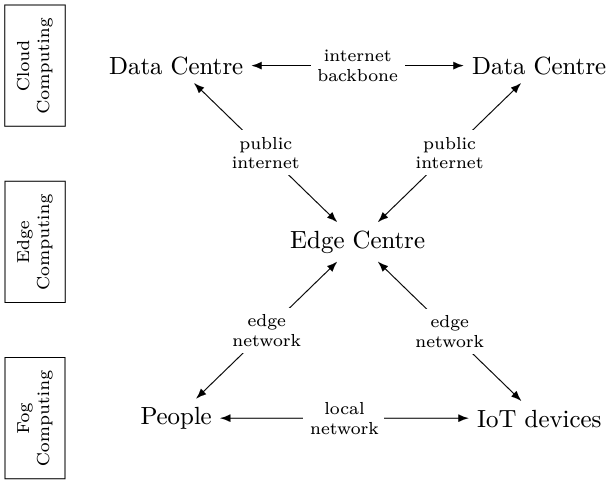
\includegraphics{images/edge_cloud_infrastructure.png}
	\caption[Panoramica sull'infrastruttura Edge Cloud]{Panoramica sull'infrastruttura Edge Cloud~\cite{berto_assurance-aware_2024}}\label{Edge cloud infrastructure}
\end{figure}

%Il continuum è il gestire sia cloud che edge come una cosa sola (in modo furbo)
In \cite{Cloud_Continuum} vengono raccolti 36 studi contenenti proposte di definizione per il \textbf{Cloud Continuum} e viene presentata come definizione complessiva \emph{``an extension of the traditional Cloud towards multiple entities (e.g., Edge, Fog, IoT) that provide analysis, processing, storage, and data generation capabilities``}.
Applicando questa definizione all'\emph{edge cloud continuum} si va a definire \emph{edge} e \emph{cloud} come entità presenti gestite come un'unica componente.
Le maggiori problematiche che il Continuum incontra con l'integrazione di nodi Edge sono dovute alla forte distribuzione geografica a cui sono soggetti gli elementi del sistema.
Le diverse distanze fisiche tra i nodi e i data-center introducono una variabilità nelle prestazioni e nella latenza a seconda della localizzazione, rendendo più difficile la capacità dei \textit{service provider} di soddisfare determinati \gls{SLA} \cite{Edge_cloud_continuum_challenges}. %https://www.queenstrl.ca/uploads/4/6/3/1/4631596/extreme_edge_computing_challenges_on_the_edge_cloud_continuum.pdf
I nodi edge richiedono anche opportune verifiche di proprietà di sicurezza e privacy, verificabili con maggiori sforzi, in quanto coinvolgono infrastrutture di terze parti.
Sorgono inoltre difficoltà nel mantenere la coerenza tra i dati in un ambiente così distribuito, vengono infatti richiesti protocolli sofisticati di sincronizzazione tra i data-center e i nodi edge che possano gestire eventuali conflitti o incongruenze derivanti dalla latenza della rete, la quale può provocare la ricezione di dati \textit{obsoleti} che comprometterebbero lo stato del sistema, e dall'elaborazione locale (dati elaborati localmente prima di essere sincronizzati col cloud). Ogni nodo possiede risorse computazionali e di storage differenti e limitate, questa eterogeneità fisica accentua la complessità nel sincronizzarsi in quanto i meccanismi e i protocolli da implementare dovranno adattarsi dinamicamente alle risorse dei vari nodi.

Nell'ambito delle infrastrutture distribuite moderne, l'Edge-Cloud Continuum rappresenta un paradigma emergente che unisce le capacità del cloud computing con l'elaborazione e l'archiviazione dati agli estremi della rete (\emph{edge computing}), il tutto in un'unico sistema complessivo (\emph{continuum}). Offre una piattaforma flessibile e scalabile che consente di distribuire le risorse computazionali tra cloud centralizzati e nodi edge situati più vicini agli utenti finali e ai dispositivi \gls{IoT}, comportando una gestione di entità distribuite geograficamente nel territorio.

Un sistema distribuito così complesso necessita tuttavia di un'adeguata soluzione per il monitoring e la verifica del suo corretto funzionamento. La natura eterogenea e geograficamente distribuita di un'infrastruttura Edge-Cloud richiede strumenti che possano garantire l'ottenimento di metriche da tutti i nodi del sistema per valutarne il relativo comportamento e rilevare anomalie o guasti, ottenendo così una soluzione di monitoring efficace.

\section{Monitoring}
In un sistema distribuito, l'affidabilità e le prestazioni dipendono dalla coordinazione e dall'integrità delle varie parti che lo compongono, rendendo il monitoraggio una pratica essenziale per garantire il corretto funzionamento dell'intero sistema. \\
Il monitoring è quella tecnica che si concentra sulla collezione di \emph{evidence}, o prove, per stabilire lo stato di salute e il comportamento del sistema. \\
Si basa su \textit{tre} elementi fondamentali:
\begin{itemize}
	\item \textbf{Logs}: registrazioni testuali di eventi che si verificano all'interno di un applicazione o di un sistema; possono includere errori, avvisi, informazioni operative e dati diagnostici. Sono informazioni strutturate in modo \textit{human-readable} in quanto pensate per essere analizzate manualmente. La gestione di grandi volumi di log provenienti da molteplici sorgenti è un problema che spesso trova soluzione nell'utilizzo di formati \textit{machine-readable} che permettono l'automatizzazione del processo di analisi.
	\item \textbf{Traces}: forniscono una visione dettagliata del percorso (\textit{trace}) che una richiesta segue in un sistema, salvando sia lo stato attuale che il relativo contesto di esecuzione. Ogni traccia è costituita da una serie di segmenti detti \textit{span} che rappresentano singole operazioni.
	\item \textbf{Metrics}: dati quantitativi che descrivono lo stato e le prestazioni di un sistema nel tempo. Includono informazioni come l'utilizzo della CPU, la memoria disponibile, il numero di richieste per secondo, la latenza delle risposte etc. Fondamentali per il monitoraggio in tempo reale e l'ottimizzazione delle prestazioni, offrono una panoramica immediata dello stato di salute del sistema.
\end{itemize}

Logs, traces e metrics sono strumenti complementari nel monitoraggio dei sistemi. Mentre i \emph{logs} forniscono un registro dettagliato degli eventi, le \emph{traces} permettono il tracciamento delle operazioni legate ad uno specifico evento a vari livelli e le \emph{metrics} consentono una misura oggettiva dello stato interno di un sistema, misure alla base della verifica di \emph{\glspl{PNF}}, approfondite nella Sezione \ref{Proprietà Non Funzionali}.

%https://www.researchgate.net/publication/3282450_Monitoring_distributed_systems#full-text
%https://dl.acm.org/doi/10.1145/13677.22723

%FORSE IL PI§ UTILE E RECENTE
%https://www.sciencedirect.com/science/article/pii/S1567832613000234

%https://ieeexplore.ieee.org/abstract/document/5557986
%https://www.sciencedirect.com/science/article/pii/S0030402615017271?casa_token=Kh33hZZHNYMAAAAA:fkpfBQJJlD3qNaCnKBY6X5OZYSNpzf-XPuEnD89EiOZ7qKiITUe0lqhGnH-XY_F9y5ZYbnHlzx8I

I primi sistemi di monitoring realizzati basati su metriche erano \textit{collettori di metriche \gls{SNMP}} il cui funzionamento è basato su un'applicazione centrale che interroga gli agenti \gls{SNMP} installati in ogni dispositivo per ottenere i dati raccolti e successivamente analizzarli. \'E un modello di monitoring completamente centralizzato e ormai superato.
La realizzazione di un sistema di monitoring attuale, invece, pone di fronte a varie scelte in merito all'architettura che il sistema andrà ad implementare, ciascuna caratterizzata da specifiche peculiarità. Alcuni esempi di scelte progettuali riguardano sia l'\textit{architettura} che l'applicativo di monitoring andrà ad avere, che l'effettivo procedimento di \textit{estrazione delle informazioni}.

\subsection{Architettura di monitoring e relative applicazioni}
Vengono analizzati alcuni esempi di tipiche architetture presenti nel mercato.
\begin{itemize}
	\item \emph{\textbf{Sistemi Completamente Centralizzati}}: sia la raccolta dei dati che il loro storage avvengono in un singolo punto centralizzato dove vengono in seguito processati e analizzati. Questo approccio fornisce semplicità, consistenza e affidabilità. Fornisce anche maggiore sicurezza e privacy in quanto i dati sono custoditi e processati in un unico ambiente. Dall'altro lato questo approccio causa alcuni svantaggi come un elevato sovraccarico del traffico di rete verso il nodo centrale e una limitata scalabilità.
	      Graylog\footnote{\label{graylog}\url{https://graylog.org/}} adotta questa architettura.

	\item \emph{\textbf{Sistemi Distribuiti}}: permettono di monitorare consistentemente i dispositivi nella rete raccogliendone le relative metriche. La raccolta ed elaborazione distribuita dei dati può ridurre la quantità di dati che devono essere trasmessi, il che può far risparmiare risorse di rete e migliorare l'efficienza. Viene inoltre migliorata la scalabilità.

	      \begin{itemize}
		      \item \emph{\textbf{Raccolta Distribuita ma Storage Centralizzato}}: i dati vengono raccolti da vari agenti o nodi distribuiti, ma vengono inviati a un punto centrale per lo storage e l'analisi. Alcuni servizi che si basano su questa architettura sono Prometheus\footnote{\label{prometheus}\url{https://prometheus.io/}} e Logstash\footnote{\url{https://www.elastic.co/logstash}}.

		      \item \emph{\textbf{Completamente Distribuito}}: sia la raccolta che lo storage dei dati sono distribuiti tra più nodi. I dati vengono memorizzati e processati in vari punti della rete, spesso con meccanismi di replica e bilanciamento del carico.
		            Alcuni servizi che si basano su questa architettura sono Elasticsearch\footnote{\label{elastic}\url{https://www.elastic.co/elasticsearch}} e Kafka\footnote{\url{https://kafka.apache.org/}}.
	      \end{itemize}
\end{itemize}

\subsection{Estrazione informazioni}\label{estrazione inforamzioni}
Un aspetto cruciale della progettazione è rappresentato dalle modalità con cui i dati o informazioni vengono estratti dai sistemi monitorati e trasferiti al sistema di raccolta e analisi. Le due modalità principali che permettono al sistema di monitoring di ottenere questi dati sono il \emph{pull} e il \emph{push}.
\begin{itemize}
	\item \textbf{Pull}: in questa modalità il sistema di monitoring richiede attivamente (\textit{polling}) i dati ai sistemi che sta monitorando; le metriche possono essere esposte sia dall'applicazione stessa (\textit{monitoring nativo}) che da \textit{agenti}, i quali si occupano di ottenere preventivamente le misurazioni.
	      \'E a tutti gli effetti una richiesta esplicita da parte del monitor verso gli \textit{endpoint} del sistema target. Un'esempio applicativo che segue questo paradigma è Prometheus\footref{prometheus}
	\item \textbf{Push}: in questa modalità il sistema di monitoring si aspetta di ricevere i dati su un interfaccia configurata per poterli elaborare; è il sistema monitorato ad inviare attivamente informazioni. Le metriche possono arrivare sia direttamente dall'applicazione che da agenti esterni. Un'esempio di applicativi che seguono questo paradigma sono Graylog\footref{graylog} e Elasticsearch\footref{elastic}
\end{itemize}

Come accennato nell'elenco, un altro aspetto legato al reperimento delle metriche riguarda la distinzione tra \emph{monitoring nativo}, detto anche \textit{agent-less}, e monitoring tramite \emph{agenti esterni}, detto \textit{agent-based}.
\begin{itemize}
	\item \textbf{Agent-based}: è una tecnica di monitoraggio che richiede l'installazione di un software, chiamato \emph{agente}, su ogni dispositivo da monitorare il quale è in grado di raccogliere e collezionare dati. Come descritto prima può essere configurato per interagire con un sistema che lavora in pull o push, rispettivamente risponde alle richieste che gli vengono fatte oppure invia autonomamente i dati. Questa metodologia, con gli adeguati permessi concessi all'agente, fornisce informazioni dettagliate sul sistema ma, dall'altro lato, utilizza un numero di risorse notabile nella macchina host e fornisce un possibile vettore di attacco aggiuntivo. Fornisce anche resilienza a problemi di rete in quanto un agente salva localmente le metriche rilevate.

	\item \textbf{Monitoring nativo o trasparente}: in questa tecnica non è necessaria l'installazione di nessun client per la raccolta dei dati sul dispositivo da monitorare ma si utilizzano strumenti e tecnologie di monitoraggio direttamente forniti all'interno delle applicazioni, evitando installazioni e configurazioni aggiuntive.
	      L'applicazione autonomamente raccoglie le proprie metriche e le espone secondo una delle modalità precedentemente elencate: può inviarle periodicamente (\emph{push}) oppure attendere di essere interrogata (\emph{pull}).
	      \'E più semplice da configurare e comporta un impatto significativamente inferiore sulle risorse del sistema host rispetto alla controparte con agenti; richiede tuttavia l'apertura di porte specifiche e dipende fortemente dalla qualità della connessione per effettuare il polling attivo dei dati.
\end{itemize}

%se no lo metto come \paragraph{}
\subsubsection{Formati e protocolli standard}\label{standard}
L'obbiettivo di ricercatori e sviluppatori è quello di utilizzare \emph{formati e protocolli standard} sia per lo scambio di dati che per la comunicazione.
Vengono garantite importanti proprietà come l'\emph{interoperabilità} tra diversi sistemi, prodotti e servizi permettendone la cooperazione senza problemi; \emph{sicurezza}, \emph{qualità} e \emph{performance} sono dovuti alle innumerevoli ricerche e utilizzi a cui una tecnologia viene sottoposta prima di essere definita standard. Altri pregi dovuti all'uso di standard sono la riduzione dei costi, sia di sviluppo che tecnologici, e la conformità legislativa ovvero il rispetto di \emph{standard legislativi} imposti.

Per integrare applicazioni e sistemi di monitoring in modo efficiente, si fa dunque largo uso di formati e protocolli standard. L'adozione di tecnologie consolidate, come l'uso di \gls{API} REST con body in formato JSON o di protocolli di rete standard come \gls{SNMP} o \emph{Syslog}, utilizzato per trasmettere e raccogliere semplici informazioni di logging dai diversi dispositivi della rete, facilita l'interoperabilità tra le applicazioni e i sistemi di monitoring, rendendo possibile l'invio e la ricezione di dati in modo standardizzato e leggibile.
Sono presenti anche standard imposti da applicativi o framework di monitoring \textit{open-source} come Prometheus\footref{prometheus} o OpenTelemetry\footnote{\url{https://opentelemetry.io/}} con il relativo \gls{OTLP} che rispettivamente trattano i dati come una time-series (flusso di valori con timestamp appartenenti alla stessa metrica) o come una struttura dati da loro definita (OpenTelemetry Model) (open-telemetry utilizza exporter che inviano i dati in  formato \gls{OTLP}, essendo uno standard viene supportato da vari servizi di monitoring come Prometheus, Jaeger, ecc).
Sono presenti anche standard per la trasmissione di metriche in ambienti \textit{cloud-native} come OpenMetrics\footnote{\url{https://openmetrics.io/}}.
Questa standardizzazione non solo semplifica l'integrazione e riduce la complessità di sviluppo, ma assicura anche una maggiore compatibilità tra diversi ambienti e piattaforme, migliorando l'efficienza operativa e la scalabilità del sistema.


\section{Proprietà Non Funzionali}\label{Proprietà Non Funzionali}
Per far fronte alle stringenti necessità di ottenere una visione sempre più completa sullo stato di un sistema sono state introdotte, al fianco delle proprietà funzionali, le \emph{\textbf{\glspl{PNF}}} il cui scopo è quello di definire \emph{come} il sistema svolge le sue funzioni concentrandosi su aspetti di \emph{qualità}, a differenza delle proprietà funzionali che definiscono \emph{cosa} effettivamente viene fornito.
Una \gls{PNF} di un sistema è un vincolo al modo in cui il sistema implementa e fornisce le sue funzionalità.
In altre pubblicazioni presenti in letteratura viene usato il termine \textit{Non Functional Requirements} riferendosi a \gls{PNF} con annesso il criterio di accettazione (requisito) da soddisfare; la metodologia adottata in questa tesi esprime formalmente i Non Functional Requirements e la loro verifica tramite Contratti, illustrati nella successiva Sezione \ref{assurance methodology}.

In questa pubblicazione \cite{review_microservices_NFR} vengono analizzati 36 paper aventi come topic le architetture a microservizi, tra questi 21 discutono le tecniche per verificare \textit{Non Functional Requirements}. La proprietà più discussa in letteratura risulta essere l'\emph{affidabilità}, seguita da \emph{scalabilità} e \emph{disponibilità}. \\
Di seguito vengono elencati e illustrati alcuni esempi di \emph{\glspl{PNF}} che possono essere misurate e valutate in un sistema.
\begin{itemize}
	%Definizioni ISO https://iso25000.com/index.php/en/iso-25000-standards
	\item \textbf{\textit{Reliability}}: affidabilità, capacità di funzionare correttamente e senza interruzioni per un determinato periodo di tempo, garantendo prestazioni stabili. \\
	Definizione ISO \cite{iso_system_quality} \textit{"Degree to which a system, product or component performs specified functions under specified conditions for a specified period of time"}.
	\item \textbf{\textit{Performance}}: prestazioni, capacità di un sistema di eseguire le sue funzionalità in modo efficiente rispettando dei requisiti e aspettative definiti dall'utente. \\
	Definizione ISO \cite{iso_system_quality} \textit{" the degree to which a product performs its functions within specified time and throughput parameters and is efficient in the use of resources (such as CPU, memory, storage, network devices, energy, materials...) under specified conditions"}.
	\item \textbf{\textit{Scalability}}: scalabilità, capacità di un sistema di gestire un aumento del carico di lavoro senza compromettere prestazioni o affidabilità. \\
	Definizione ISO \cite{iso_system_quality} \textit{"Degree to which a product can handle growing or shrinking workloads or to adapt its capacity to handle variability"}.
	\item \textbf{\textit{CIA - Confidentiality}}: confidenzialità, garantisce che i dati vengano acceduti solo da chi effettivamente autorizzato e non vengano divulgati. \\
	Definizione ISO \cite{iso_system_quality} \textit{"Degree to which a product or system ensures that data are accessible only to those authorized to have access"}.
	\item \textbf{\textit{CIA - Integrity}}: integrità, garantisce che i dati siano accurati, completi e non alterati in modo non autorizzato; in altre parole i dati sono corretti e attendibili. \\
	Definizione ISO \cite{iso_system_quality} \textit{"Degree to which a system, product or component ensures that the state of its system and data are protected from unauthorized modification or deletion either by malicious action or computer error"}.
	\item \textbf{\textit{CIA - Availability}}: disponibilità, il sistema è accessibile e operativo quando richiesto. \\
	Definizione ISO \cite{iso_system_quality} \textit{"Degree to which a system, product or component is operational and accessible when required for use"}.
	\item \textbf{\textit{Access control}}: controllo accessi, solo gli utenti autorizzati dalle politiche del sistema possono accedere alle risorse
	\item \textbf{\textit{Resilience}}: resilienza, capacità di un sistema di continuare a funzionare correttamente, e di recuperare rapidamente, in seguito ad un guasto. \\
	Definizione ISO \cite{iso_system_quality} \textit{"Degree to which a product can automatically place itself in a safe operating mode, or to revert to a safe condition in the event of a failure"}.
\end{itemize}

\'E importante sottolineare il fatto che queste proprietà definiscono degli obbiettivi concettuali da raggiungere ma non trattano le modalità con cui si verifica l'effettivo soddisfacimento. Questo accade perché le modalità di verifica differiscono in base all'entità che si sta controllando ed è compito di un \textit{esperto del sistema}, colui che ha adeguate conoscenze e competenze, andare a definire come una proprietà si può concretizzare in uno specifico contesto.
%cambiare definire
Gli esempi illustreranno come l'espressione pratica dello stesso concetto è strettamente legata al contesto di applicazione.

\begin{exmp}
	Valutando l'\textit{availability} di un server si misura il tempo durante il quale il server è \textit{up} e funziona correttamente (riceve le richieste e risponde fornendo il relativo servizio) mentre valutando l'\textit{availability} di una rete cellulare si va a misurare la capacità della rete di fornire connessione ai dispositivi mobili in una determinata area geografica.
\end{exmp}

\begin{exmp}
	Valutando l'\textit{Integrity} di una comunicazione di rete ci si riferisce alla capacità di trasmettere e ricevere i dati senza alterazioni o perdite mentre valutando l'\textit{Integrity} di uno \textit{storage} (come un database o un dispositivo di archiviazione fisico) ci si riferisce alla capacità di garantire che i dati archiviati non vengano alterati e rimangano completi.
\end{exmp}

\section{Verifica di Proprietà non Funzionali - Assurance}\label{Verifica di PNF}
Le tecniche di \textbf{assurance} mirano a garantire che un sistema \emph{verifichi}, e quindi soddisfi, determinate Proprietà Non Funzionali precedentemente definite. \\
Per questa tesi viene adottata la \emph{\textbf{metodologia di assurance}} utilizzata in \cite{berto_assurance-aware_2024}, e riportata in questa sezione, che si occupa di misurare e valutare \glspl{PNF} di un'infrastruttura target sulla base delle \textit{evidence} raccolte dagli endpoint di monitoring. La verifica viene formalizzata attraverso l'uso di contratti basati sulle \textit{evidence} raccolte.
Questa metodologia adottata per il processo di \emph{assurance} mira a valutare un sistema indipendentemente dallo stato in cui si trova durante la valutazione (valutazione statica) basando i suoi risultati su misurazioni raccolte, archiviate in uno storage e indicizzate nel tempo invece che su misure dirette, permettendo così la definizione di contratti basati su intervalli temporali.

Ogni componente del sistema possiede uno \emph{stato interno}, rappresentazione dinamica dello stato delle variabili e delle risorse, e una \emph{configurazione}, configurazione statica del componente che ne caratterizza il comportamento, utilizzati per valutarne determinate proprietà.
Questi due dati (stato interno e configurazione) vengono esposti dal componente del sistema al processo di assurance tramite interfacce di monitoring standard dette anche \emph{endpoint di monitoring}.
Gli endpoint andranno a rappresentare il target del processo di assurance per la raccolta di \textit{measurements} dall'infrastruttura.

\subsection{Assurance methodology}\label{assurance methodology}

\begin{figure}[th]
	\centering
	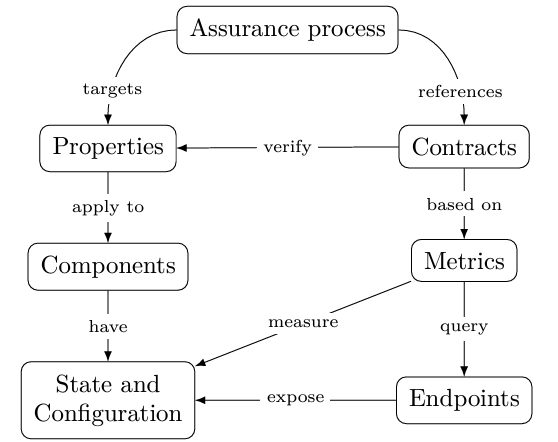
\includegraphics{images/assurance_methodology.png}
	\caption[Schema di \emph{assurance methodology}]{Schema di \emph{assurance methodology} proposto in~\cite{berto_assurance-aware_2024}}\label{Schema assurance methodology}
\end{figure}

La Figura \ref{Schema assurance methodology} mostra lo schema della metodologia di assurance che verrà utilizzato nel corso di questa tesi. \\
La metodologia adottata in \cite{berto_assurance-aware_2024} utilizza gli endpoint delle infrastrutture come fonte di misurazioni (espongono lo stato e le configurazioni del sistema).
Le misurazioni degli endpoint vengono valutate attraverso \textbf{metriche} le quali si focalizzano sulla valutazione di un comportamento specifico per verificare \glspl{PNF}.
Le metriche, una volta valutate e ottenute le relative \textit{evidence}, diventano la base per la valutazione dei \textbf{contratti}, i quali fanno riferimento direttamente a una \gls{PNF} specifica e descrivono come può essere verificata in modo formale.
Individuiamo nelle \emph{metriche} e nei relativi \emph{contratti} gli elementi focali di questa sezione.

\paragraph{Metriche}
Una metrica è una funzione associata da una funzionalità, la quale vuole misurare i suoi aspetti o comportamenti sui componenti che la implementano; è un \textit{qualsiasi tipo di trasformazione che viene applicato ai dati} per trasformarli in una forma più utile. La più semplice trasformazione, definita identità, consiste nel tenere i dati grezzi ``così come sono``.
Esistono poi trasformazioni che vanno a ridurre la quantità di dati raccolti rispetto al totale reperibile dal sistema, mirando ad estrarre proprietà o informazioni specifiche da essi.
Vengono definite sugli stati e sulle configurazioni esposte dagli endpoint di monitoring. La valutazione delle metriche fornisce le \textit{\textbf{evidence}}, o prove, misurazione oggettive atte a confermare se una particolare proprietà è valida.

\paragraph{Contratti}
Descrivono formalmente come validare le proprietà di un servizio. Un contratto è una funzione booleana il cui scopo è quello di valutare la validità o meno di una determinata proprietà. La valutazione avviene basandosi sulle \textit{evidence}, o prove, ottenute tramite valutazione delle metriche degli endpoint.
Un contratto è una tupla costituita dal \emph{istante di tempo} in cui è avvenuta la valutazione e dal \emph{set di componenti} che implementano il servizio target.
Un aspetto cruciale dei contratti è essere \textit{time-dependant}, l'esito dipende quindi dall'istante temporale in cui è stato valutato il contratto.
Per garantire consistenza, questa metodologia mira a definire un solo contratto per ogni proprietà (mapping bigettivo tra proprietà e contratto).

\subsection{Assurance process}\label{assurance process}
\begin{figure}[th]
	\centering
	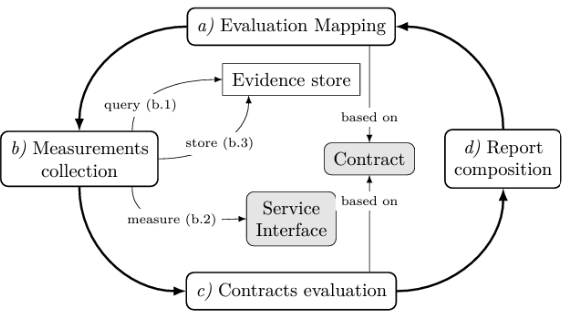
\includegraphics{images/assurance_process.png}
	\caption[Schema di \emph{assurance process}]{Schema di \emph{assurance process} proposto in\cite{berto_assurance-aware_2024}}\label{Assurance process}
\end{figure}
%https://ieeexplore.ieee.org/stamp/stamp.jsp?tp=&arnumber=9750109
Un processo di assurance dipende da una \emph{assurance methodology} per validare le proprietà.
La soluzione adottata in \cite{berto_assurance-aware_2024} supporta la verifica continua e collaborativa di \glspl{PNF} delle componenti infrastrutturali.
La Figura \ref{Assurance process} applica l'\emph{assurance methodology} vista nella Sezione \ref{assurance methodology} suddividendo il processo in 4 step ripetuti ciclicamente.
\begin{enumerate}[label=(\alph*)]
	\item \emph{Evaluation mapping}: nel primo step, partendo dalle \emph{proprietà} che si intendono verificare si va ad identificare le \emph{metriche} e i \emph{contratti} che dovranno essere valutati per poter effettuare quegli accertamenti

	\item \emph{\textbf{Measurement} collection}: il passo successivo consiste nella valutazione  delle metriche (\textit{metrics evaluation}) precedentemente identificate e fornite dal servizio, step b.2, e nella seguente raccolta e immagazzinamento delle \textit{evidence} generate (\textit{measurements}), step b.3.

	\item \emph{\textbf{Contracts} evaluation}: nel terzo passaggio viene eseguita l'effettiva verifica delle proprietà, calcolando il risultato del \emph{contratto}, utilizzando le misurazioni raccolte in precedenza (\textit{measurements} usate come \textit{evidence} per comprovare un contratto) e restituendo un output booleano.

	\item \emph{Report composition}: nell'ultimo passaggio i risultati parziali, \emph{measurements} e \emph{contracts evaluation}, vengono aggregati in un report che include una descrizione dei risultati (proprietà verificate o no) e le relative \textit{evidence} a supporto. Il report viene generato seguendo un formato \textit{machine readable} per garantirne il facile utilizzo in altri processi automatizzati, come la certificazione descritta nella sezione successiva.
\end{enumerate}


\section{Certificazione di Proprietà non Funzionali - Certification}
La \textbf{certificazione} è una tecnica di \textit{security assurance} il cui scopo è dimostrare, seguendo uno \emph{schema di certificazione}, che un sistema target, in un determinato istante di tempo, si comporti come previsto e soddisfi determinate \glspl{PNF}. Il funzionamento è costituito in parte dalla \emph{verifica di \glspl{PNF}} precedentemente illustrata nella Sezione \ref{Verifica di PNF} ma con l'aggiunta di una \gls{CA} il cui compito è la gestione sicura del processo di verifica garantendo sicurezza, affidabilità e ripetibilità.
La certificazione, come menzionato in \cite{certification_sw_development}, è stata integrata nel ciclo di vita dei sistemi distribuiti, partendo dallo sviluppo degli stessi, per aumentare la qualità del servizio e garantire un comportamento stabile nel tempo.

\begin{figure}[th]
	\centering
	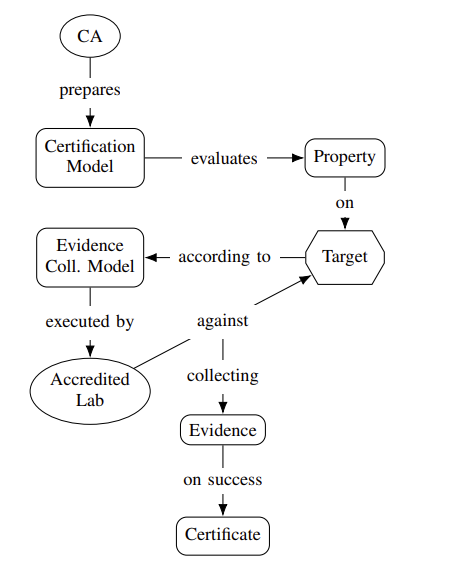
\includegraphics{images/certification_process}
	\caption[Generico processo di certificazione]{Generico processo di certificazione~\cite{NF_certification_distributed_system}}\label{Generico processo di certificazione}
\end{figure}

%vedi questa citazione https://dl.acm.org/doi/10.1145/2767005

Per questa tesi viene adottata la metodologia menzionata in Ardagna et al.\ \cite{NF_certification_distributed_system} utilizzando la loro nomenclatura.
La Figura \ref{Generico processo di certificazione} mostra un generico schema di certificazione contenente le entità coinvolte (\gls{CA}, \gls{AL} e Target) e le varie interazioni per giungere ad un certificato. \'E fondamentale la creazione di una \textit{chain-of-trust} tra l'\textit{utente} che chiede la certificazione, la \gls{CA} che prepara il \textit{certification model}, l'\gls{AL} che esegue il \textit{certification model} e il certificato rilasciato.
Segue un'illustrazione delle componenti presenti nello schema.

\paragraph{Target}
rappresenta l'obbiettivo del processo di certificazione ed è costituito dalle implementazioni concrete dei componenti del sistema a cui il certificato è rivolto (un software, un servizio o un sistema in senso più ampio).

\paragraph{\gls{CA}}
Ha il compito di definire e orientare tutte le attività necessarie per valutare e certificare una specifica proprietà su un Target; lo fa definendo un \emph{Certification Model} che contiene un \emph{Evidence Collection Model}.
Fornisce delle linee guida fondamentali per assicurare che il processo di certificazione sia condotto in modo sistematico e conforme ai requisiti predefiniti garantendo sicurezza e affidabilità.

\subparagraph{Certification Model}
Una specifica delle attività da eseguire per certificare \glspl{PNF} sul sistema target.
Il modo più conciso di rappresentarlo è una tupla costituita da \emph{Proprietà} che si intendono verificare, \emph{Target} ed \emph{Evidence Collection Model}. \'E parte fondamentale di un certificato in quanto definisce cosa si sta certificando (proprietà), come (\emph{evidence collection model}) e chi si sta certificando (target) andando a definire concretamente come deve avvenire la certificazione.

\subparagraph{Evidence}
tutti i dati raccolti e valutati i modo oggettivo su un sistema target, include sia i dati delle metriche che le valutazioni fatte

\subparagraph{Evidence Collection Model}
coordina le attività necessarie a raccogliere \textit{evidence} dal sistema target, le quali verranno valutate per stabilire il rilascio del certificato o meno.
Definisce come i dati raccolti dal sistema di monitoring vanno all'\gls{AL}.

\paragraph{\gls{AL}}
sono laboratori riconosciuti ufficialmente da un ente di accertamento e richiedono di rispettare determinate norme (ad esempio \textit{\cite{iso_testing}: General requirements for the competence of testing and calibration laboratories}) per garantire affidabilità e precisione dei risultati.
Viene delegato dalla \gls{CA} per eseguire l'\emph{Evidence Collection Model} sul sistema target; con i dati raccolti, le \textit{evidence}, il laboratorio potrà assegnare un certificato al sistema in caso di valutazione positiva %vedi citazione https://ieeexplore.ieee.org/document/9844845


\paragraph{Certificato}
il certificato viene rilasciato dalla CA ai sistemi target che superano con successo la valutazione di determinate \glspl{PNF} sulla base delle \emph{evidence} raccolte, ne attesta la conformità. Contiene un riferimento al \textit{certification model}, il quale ne illustra i dettagli, e alle \textit{evidence} raccolte che ne supportano la validità.

\paragraph{Flusso di esecuzione:} La \gls{CA} definisce il \emph{Certification Model} costituito dalle proprietà che devono essere verificate su un sistema target seguendo uno specifico \emph{Evidence Collection Model}. L'\gls{AL}, delegato dalla \gls{CA}, ha l'incarico di raccogliere le prove o \textit{evidence} dal sistema.
Se le \emph{evidence} dimostrano positivamente la conformità della proprietà viene rilasciato un \emph{certificato} che attesta la conformità del sistema ai requisiti stabiliti.


\section{Related Work}
%In [] viene proposta una metodologia basata su ... il cui scopo è ... \\
%(2014)
In \cite{Multi_layer_Cloud_Assurance_Evaluation_methodology} viene proposta una metodologia di valutazione multi-layer (monitora il livello fisico, le VM e le applicazioni in esecuzione sulle VM raccogliendo metriche a vari livelli di granularità) e continua, fondata sui \gls{CC}\footnote{https://www.commoncriteriaportal.org/}, per valutare i livelli di sicurezza delle applicazioni Cloud, in termini di Assurance Level, attraverso l'aggregazione delle proprietà di sicurezza, raccolte su vari livelli, dei singoli componenti che le costituiscono.
Fornisce al proprietario del servizio una panoramica della sicurezza del suo servizio senza la necessità di analisi manuali dettagliate.

%(2016)
In \cite{certification_cloud_services} viene proposto un framework di certificazione della sicurezza test-based (test-based assurance: le evidence arrivano da test e non da strumenti di monitoring) per servizi cloud.
Fornisce una metodologia e un ambiente di cloud-engineering basati su certificati con il relativo set di componenti che gestisce il processo di certificazione, online e semi-automatico, di servizi/applicazioni in un sistema cloud-based; fornisce anche dei tools in supporto alla chain-of-trust imposta dalla certificazione.
Il framework infine supporta la valutazione di sistemi cloud sia pre-deployment che in production-deployment a diversi livelli, discostandosi dai tradizionali strumenti che non considerano il processo di sviluppo.

%(2020)
In \cite{semiautomatic_continuous_cloud_certification} viene proposta una rigorosa e adattiva tecnica di assurance basata sulla certificazione che mira ad un ecosistema cloud trasparente ed affidabile dove ogni parte del cloud si comporta come previsto.
Utilizza uno schema di certificazione basato su test per dimostrare il soddisfacimento di \gls{PNF} dei servizi cloud; una \gls{CA}, online e disponibile durante l'intero processo, definisce i requisiti non funzionali da verificare su un determinato modello. Il controllo avviene in modo semi-automatico tramite un algoritmo di matching che effettua un confronto tra il certification model definito dalla CA e un'istanza.
Presenta inoltre un processo continuo e incrementale di gestione del ciclo di vita di un certificato (semi-)automatico, dall'emissione al suo riadattamento a cambi contestuali (cloud multilayer dinamici) alla revoca.
Il framework è stato applicato in uno scenario industriale reale per la gestione di un sistema di pagamento (ENGpay) e ne sono state valutate prestazioni, qualità, applicabilità e usabilità pratica.
%OPTIONAL TODO
%\hl{
%posso collegarlo alla citazione sopra dicendo che è un paper specifico che parla dei cambi nei sistemi (questo è del 2023 quello sopra del 2020 quindi ha senso)
%https://air.unimi.it/handle/2434/1018841: Continuous Certification of Non-functional Properties Across System Changes
%}

%(2021)
In \cite{assurance_risk_managament_ds} viene proposto un framework di gestione del rischio per sistemi distribuiti basato su tecniche di \emph{assurance}, le quali monitorano il comportamento del sistema tramite valutazione di \gls{PNF}, che soddisfa i requisiti di \emph{gestione del rischio} imposti dai moderni sistemi distribuiti; statistiche come performance e qualità del framework sono state misurate in uno scenario simulato di industria 4.0.
Questo framework fornisce un espansione ai framework di risk-management consentendo alle organizzazioni grandi e complesse di valutare il proprio rischio basandosi su risultati derivanti dalla valutazione di \gls{PNF} relativi all'efficacia dei meccanismi implementati, integrando quindi completamente il concetto di \emph{assurance} alla gestione del rischio.

In questi due paper vengono proposti studi in merito all'\textbf{assurance in dispositivi \gls{IoT}} le cui ricerche rispetto a servizi e sistemi cloud sono ancora agli inizi. \\
%(2021)
In \cite{assurance_framework_edge_iot} viene proposto un framework altamente automatizzato di security assurance per sistemi Edge e \gls{IoT}, paradigmi di elaborazioni emersi negli ultimi anni, indipendente dalle complessità infrastrutturali e basato su un'architettura di Kubernetes avanzata in grado di gestire applicazioni 5G-native.
Implementa un processo di assurance altamente scalabile che garantisce la verifica di \gls{PNF} raccogliendo evidence dal sistema target.
Come caso reale di applicazione viene presentato l'\gls{IoMT} considerano come contesto di esecuzione un moderno ospedale dotato di molti device eterogenei (sensori umidità e temperatura, dispositivi \gls{IoT} medici ecc). \\
%(2022)
L'anno successivo in \cite{assurance_iot} il framework proposto in precedenza viene ampliato introducendo il concetto di assurance \gls{IoT} guidata da una visione olistica del sistema di destinazione.
Questo metodo definisce ed esegue valutazioni di assurance che si allineano e sfruttano l'architettura del sistema target, distribuendo e aggregando i calcoli di conseguenza.
Il framework considera l'intero ciclo di vita del sistema e produce risultati a diversa granularità attraverso una valutazione di assurance basata su attività multi-layer, multifase (in diversi momenti del suo ciclo di vita) e comportamentali.
Il framework proposto è stato valutato in uno \emph{Smart Light System} reale.

%(2023)
Come visto in \cite{NF_certification_distributed_system}, la certificazione di moderni sistemi distribuiti incontra alcune \emph{difficoltà} dovute sia al continuo adattamento ed evoluzione dei sistemi, implicando l'invalidamento dei corrispondenti certificati (la cui realizzazione richiede sforzo in termini di tempo e risorse), che alla presenza di \gls{ML} a livello applicativo e infrastrutturale. Queste caratteristiche rendono il comportamento del sistema impredicibile, in contrasto con i principi fondanti della certificazione quali \emph{staticità, predicibilità e verificabilità}.


%TOP spiegazione certificazione
%(2023)
Lo schema di certificazione proposto in \cite{multi_dimensional_certification_ds} va oltre la semplice valutazione del comportamento di un servizio, prendendo in considerazione fattori aggiuntivi che descrivono, ad esempio, come il servizio è stato implementato e verificato, con l'obiettivo di aumentare la qualità e le prestazioni di un sistema distribuito.
Questo approccio è definito certificazione multidimensionale, poiché include dimensioni aggiuntive che modellano aspetti rilevanti (ad esempio, linguaggi di programmazione e processi di sviluppo) che contribuiscono in modo significativo alla qualità dei risultati della certificazione; l'obiettivo non si limita più alla valutazione delle \gls{PNF} degli artefatti software ma viene esteso per considerare \emph{dimensioni} aggiuntive, come ad esempio i processi di sviluppo e verifica.
Questo schema certifica le proprietà di un dato servizio considerando ogni dimensione in modo indipendente:
compone i risultati della valutazione in ogni dimensione e produce un certificato accurato del comportamento del servizio.
Lo schema infine è integrato nella gestione del ciclo di vita (dallo sviluppo del sistema al suo funzionamento e alla sua manutenzione) di sistemi distribuiti per supportare una selezione dei servizi basata sulla certificazione, in cui i servizi funzionalmente equivalenti vengono classificati (service ranking) in base alle \gls{PNF} certificate che detengono e ai requisiti degli utenti corrispondenti, utilizzando una tecnica di Multi-Criteria Decision-Making (MCDM).
Questa modellazione porta a certificati più accurati e, di conseguenza, a un processo decisionale più accurato quando i servizi/software vengono selezionati dinamicamente in fase di esecuzione sulla base dei loro certificati. \\
In conclusione questo approccio offre vantaggi per tutte le parti coinvolte: i fornitori di servizi ottengono certificati che riflettono meglio tutte le best practice seguite; gli utenti finali possono fare scelte più consapevoli grazie a certificati dettagliati e ben strutturati; la CA fornisce uno schema di certificazione più utile.


%https://air.unimi.it/retrieve/dfa8b99d-09e9-748b-e053-3a05fe0a3a96/main.pdf : Test-Based Security Certification of Composite Services


%https://air.unimi.it/handle/2434/554823: "Certification-Based Cloud Adaptation"
%Ardagna et al. [136] described a lightweight certification methodology for cloud environments, supported by continuous monitoring of infrastructures, platforms and services.

%https://air.unimi.it/handle/2434/371230: Security certification for the Cloud: the CUMULUS approach

%https://air.unimi.it/handle/2434/921233: A security certification scheme for Information-Centric Networks: proposed a formal certification scheme to validate NFPs cloud-based services.

%https://air.unimi.it/retrieve/handle/2434/888053:
%“Security Certification Scheme for Content-centric Networks,

\chapter{Implementazione}\label{implementazione}

In questo capitolo viene descritto il processo di implementazione della soluzione proposta per la valutazione di sistemi distribuiti. L'obiettivo principale è illustrare i dettagli dell'infrastruttura creata, i componenti utilizzati e il funzionamento generale del sistema. \\
La prima parte si concentra sul \emph{target} dell'assurance, ovvero l'ambito dei servizi e delle applicazioni monitorati.
Successivamente, si descrive l'\emph{infrastruttura sperimentale} utilizzata per il deployment basata su MicroK8s.
La parte centrale del capitolo si focalizza sul deployment e sul funzionamento dello \emph{stack} fornito da \emph{Elasticsearch}.
Infine si tratta l'\emph{Assurance Engine}, ovvero il framework di monitoring in corso di sviluppo.

\section{Assurance Target}
Il sistema implementato ha come \textit{scope}, ovvero obbiettivo di monitoring, una determinata tipologia di servizi, concentrandosi su applicazioni o \gls{VM} containerizzate e deployate all'interno del cluster Kubernetes del laboratorio. In altre parole, il target del sistema sono esclusivamente entità (applicazioni o \gls{VM}) distribuite internamente al cluster, che possono presentare una struttura centralizzata o distribuita.
Le entità classificabili come possibili esempi di target vanno dai generici servizio deployabili in un cluster kubernetes come un web server o un database ad entità più specifiche come il servizio di GitLab\footnote{\url{https://about.gitlab.com/}} fino ad arrivare a sistemi operativi completamente deployati (\gls{VM}) sul cluster tramite l'utilizzo di KubeVirt\footnote{\url{https://kubevirt.io/}}.

Una delle caratteristiche più rilevanti di questo sistema è la capacità di monitorare sia entità predisposte al monitoring trasparente, sia entità che richiedono l'ausilio di agenti per il monitoraggio, come descritto nella Sezione \ref{estrazione inforamzioni}.
La flessibilità di questo approccio permette di superare un'importante limitazione del monitoring, consentendo la raccolta di dati da entità distribuite eseguite in container, pur non avendo un controllo diretto sul loro funzionamento in quanto si tratta di servizi o applicazioni prodotti da enti terze, ``pronti all'uso'' e con un'interfaccia di tipo \textit{black-box}.
Il sistema è quindi in grado di monitorare ogni tipo di applicativo distribuito all'interno del cluster. Questa integrazione è ulteriormente facilitata dalle \emph{integrazioni} native che \emph{Elasticsearch} mette a disposizione per interfacciarsi con vari servizi o applicativi standard, come Kubernetes o servizi offerti da Apache e \gls{AWS}, ecc.

\section{Experimental setup}
In questa sezione verrà descritto l'ambiente Kubernetes utilizzato per l'implementazione e lo sviluppo del sistema, con un'analisi delle sue configurazioni e componenti principali.

Il cluster è stato sviluppato tramite \textbf{MicroK8s}\footnote{\url{https://microk8s.io/}}, una distribuzione \textit{lightweight} di Kubernetes sviluppata da Canonical\footnote{\url{https://canonical.com/}} e progettata per essere facilmente installabile ed eseguibile.
MicroK8s è caratterizzato da un'architettura modulare che consente agli utenti di attivare solo i componenti necessari per il proprio ambiente.
L'installazione predefinita include un cluster Kubernetes completamente funzionante, con l'opzione di aggiungere delle componenti (add-ons) come DNS, ingress, dashboard, e altri servizi comuni tramite semplici comandi.
Fornisce quindi un cluster Kubernetes facilmente componibile.
Il pacchetto include anche il supporto per il deployment di cluster distribuiti, noti anche come cluster multi-nodo. \\
L'infrastruttura sperimentale è quindi costituita da un cluster Kubernetes deployato tramite MicroK8s su 3 nodi fisici eterogenei presenti nel laboratorio, ognuno dei quali possiede differenti capacità in termini computazionali e di storage.
Nella Tabella~\ref{risorse nodi} vengono indicate le specifiche di ogni nodo presente, in questo modo l'architettura del sistema diventa replicabile permettendo l'esecuzione di esperimenti su un setup identico.

%https://tex.stackexchange.com/questions/60601/evenly-distributing-column-widths

%\textbf{CPU Core} & \textbf{Frequenze}
\begin{table}[h!]
	\caption{Risorse disponibili nel sistema}\label{risorse nodi}
	\centering
	\begin{tabularx} {\textwidth}
		{c*{6}{C}} % C è un column type definiti nel main
		\toprule
		\multirow{2}{*}{\textbf{Nodo}} & \multicolumn{3}{c}{\textbf{CPU}} & \multirow{2}{*}{\textbf{RAM}} & \multirow{2}{*}{\textbf{Disco}}                                                     \\

		\cmidrule(r){2-4} %permette di estendere solo sotto alcune colonne definite multi column
		                               & \textbf{Modello}                 & \textbf{Core}                 & \textbf{Frequenza}                                                                  \\
		\midrule
		balthasar                      & Broadwell                        & 16                            & 2.10 GHz                        & 15.6 GiB                 & 296.8 GiB                \\
		casper                         & Broadwell                        & 16                            & 2.10 GHz                        & 23.4 GiB                 & 296.8 GiB                \\
		\multirow{2}{*}{melchior}      & \multirow{2}{*}{EPYC 7453}       & 28                            & 2.75 GHz                        & \multirow{2}{*}{252 GiB} & \multirow{2}{*}{1.7 TiB} \\
		                               &                                  & 28                            & 2.75 GHz                        &                         &                         \\

		\bottomrule
		Totale                         &                                  & 88                            &                                 & 291 GiB                 & 2.3 TiB                  \\
		\bottomrule
	\end{tabularx}
\end{table}

Per la gestione dello \textbf{storage distribuito}, il cluster utilizza Longhorn\footnote{\url{https://longhorn.io/}}, un un sistema di storage a blocchi distribuito (\textit{distributed block storage system}) e \textit{open-source}.
Fornisce \emph{volumi persistenti} altamente disponibili e affidabili attraverso la loro \emph{replica} archiviata su più nodi, assicurando così la continuità del servizio anche in caso di failure hardware o di rete (no \textit{single-point-of-failure}).
Grazie alla sua architettura leggera e all'integrazione nativa con Kubernetes, Longhorn semplifica la gestione dello storage dinamico e scalabile, supportando operazioni come il provisioning automatico dei volumi.
Una delle caratteristiche chiave offerte da Longhorn sono le funzionalità di \emph{backup} e \emph{snapshot} \emph{incrementali}, facilmente gestibili attraverso la sua interfaccia utente.
Le snapshot consentono di catturare lo stato dei volumi in determinati momenti nel tempo, facilitando il ripristino rapido dei dati in caso di errori o corruzione (system side) o per la creazione di repliche.
I backup, invece, permettono di salvare copie dei dati su storage esterni al cluster basandosi sugli snapshot, aumentando ulteriormente la sicurezza e la durabilità delle informazioni critiche (user side).
Queste funzionalità contribuiscono a garantire l'integrità e la disponibilità dei dati del \textit{persistent volume storage} sia all'interno che all'esterno del cluster Kubernetes, supportando strategie di disaster recovery efficaci e riducendo il rischio di perdita di dati.

Il cluster utilizza anche un plugin \textbf{\gls{CNI}}, che si occupa di configurare dinamicamente le risorse di rete e rimuoverle dai container terminati, per gestire il networking interno.
Il plugin installato è Kube-ovn\footnote{\url{https://www.kube-ovn.io/}}, una soluzione avanzata e performante che combina le capacità di Kubernetes con le ricche e comprovate funzionalità di virtualizzazione di rete basate su \gls{OVN}\footnote{\url{https://www.ovn.org/}}, una piattaforma per il \gls{SDN}, in un ambiente \textit{cloud-native}; consente la creazione di reti logiche e virtuali che si sovrappongono all'infrastruttura fisica esistente.
\gls{OVN} si costituisce come una serie di \textit{daemon} per \textit{Open vSwitch}\footnote{\url{https://www.openvswitch.org/}} che traducono le configurazioni di rete virtuale in \textit{OpenFlow}, un protocollo di comunicazione che permette la gestione del flusso di dati all'interno di switch e router in reti software-defined.
Fornisce quindi un maggiore controllo sullo switching/routing dei pacchetti nella rete e sul binding delle porte logiche. Consente inoltre la specifica di policy di sicurezza avanzate (Firewall) e un controllo completo sulla rete (\textit{load-balancing, Quality of Service, monitoring}).
L'approccio \gls{SDN} consente una gestione delle reti che separa il \textit{control plane} della rete, la logica che decide la topologia di rete e le informazioni nelle routing tables, dal \textit{data-plane}, che si occupa dell'effettivo inoltro del traffico, consentendo una gestione programmabile e centralizzata della rete, la quale diventa più flessibile e dinamica adattandosi alle esigenze.


Il cluster di riferimento gestisce tutte le entità, siano esse servizi o \gls{VM}, come risorse di calcolo e storage creando uno strato di astrazione al di sopra di esse che consente di generalizzarne l'aspetto. Questa infrastruttura distribuita su vari nodi e con componenti eterogenee rappresenta uno scenario ideale per \textbf{test realistici}, grazie alla sua capacità di rispecchiare ambienti applicativi complessi e variabili.

\section{ECK Stack}
La prima fase dell'implementazione è costituita dal deployment dello stack \gls{ECK}\footnote{\url{https://artifacthub.io/packages/helm/elastic/eck-stack}} che estende le funzionalità di orchestrazione di base di Kubernetes per supportare la configurazione e la gestione di Elasticsearch, Kibana, Elastic Agent, Fleet Server, ecc.
Segue un'illustrazione delle varie componenti deployate.

\paragraph{Elasticsearch}
il cuore dello stack Elastic, è un archivio dati scalabile e distribuito con implementato un motore di ricerca e analisi utilizzabile tramite query presso le \gls{API} RESTful che espone. La sua architettura distribuita permette di scalare orizzontalmente, distribuendo il carico di lavoro su più nodi, garantendo così elevata disponibilità e prestazioni.
Viene utilizzato per cercare, indicizzare, archiviare e analizzare dati di tutte le forme in tempo reale date le ottimizzazioni in termini di performance.

\paragraph{Kibana}
è la \gls{GUI} progettata per \emph{visualizzare e osservare}, \emph{cercare}, \emph{analizzare} e \emph{gestire} i dati archiviati in Elasticsearch. Fornisce strumenti per creare dashboard, grafici, tabelle e mappe interattive, eseguire ricerche avanzate e monitorare in tempo reale i dati.

\paragraph{Elastic Agent}
rappresentano una singola e unificata modalità per aggiungere monitoring per log, metriche e altri tipi di dati a un host, semplificando e velocizzando l'implementazione nell'intera infrastruttura. Forniscono anche funzionalità di protezione dell'host da minacce di sicurezza.
Elastic fornisce delle \emph{Integration} per gli agent, ovvero una raccolta di asset che definiscono come collegarsi ad uno specifico prodotto o servizio esterno attraverso lo Stack Elastic, raccogliendo, archiviando e visualizzando facilmente qualsiasi dato da qualsiasi fonte. Forniscono inoltre risorse pronte all'uso come dashboard, visualizzazioni e pipeline per estrarre campi strutturati da log ed eventi provenienti da questi servizi.
Infine, ogni agente ha una singola policy che può essere aggiornata per aggiungere integrazioni per nuove fonti di dati e protezioni di sicurezza.

\paragraph{Fleet}
è un componente che fornisce gestione centralizzata degli Elastic Agent e delle relative policy attraverso una specifica interfaccia utente di Kibana.
Fleet funge da canale di comunicazione per gli Elastic Agent, i quali effettuano regolarmente il \textit{check-in} per aggiornamenti e comunicando il relativo stato di salute. Quando viene apportata una modifica a una policy o ad una integrazione, tutti gli agenti ricevono l'aggiornamento durante il \textit{check-in} successivo senza necessità di intervento manuale.

\subsection{Deployment}
Lo stack è reso disponibile tramite Helm\footnote{\url{https://helm.sh/}}, un package-manager per Kubernetes che semplifica la definizione, l'installazione, l'upgrade e la gestione di applicazioni su un cluster. Si basa su \emph{chart}, pacchetti preconfigurati di risorse Kubernetes che permettono di automatizzare e standardizzare il deployment di applicazioni, riducendo la complessità e migliorando la consistenza tra ambienti.
Gli \emph{helm chart} da deployare sono tre: \texttt{eck-operator}\footnote{\url{https://artifacthub.io/packages/helm/elastic/eck-operator}}, \texttt{eck-stack}\footnote{\url{https://artifacthub.io/packages/helm/elastic/eck-stack}} e \texttt{kube-state-metrics}\footnote{\url{https://artifacthub.io/packages/helm/bitnami/kube-state-metrics}}.

\paragraph{eck-operator}
è il componente che si occupa di automatizzare il deployment, la gestione e l'orchestrazione di tutto lo stack \gls{ECK} e quindi, nel nostro contesto, di Elasticsearch, Kibana e degli Elastic Agent.
Il deployment non prevede configurazioni particolari e può essere fatto attraverso: \texttt{helm install my-eck-operator elastic/eck-operator}

\paragraph{eck-stack}
è il chart che contiene tutti i componenti deployabili dello stack;
si pone come l'aggregazione di 6 chart corrispondenti ai 6 applicativi offerti. Nel dettaglio sono eck-elasticsearch, eck-kibana, eck-agent, eck-fleet-server, eck-logstash ed infine eck-apm-server. \\
La configurazione di default abilita solo Elasticsearch e Kibana, in quanto servizi esistenziali dello stack, ma per il nostro caso di studio dovranno essere abilitati anche gli Agent e il Fleet Server.
Dopo aver selezionato i servizi da deployare è necessario andare a configurare singolarmente ciascuno di essi, andando ad impostare opportunamente i \textit{values} offerti dal relativo chart.

\paragraph{kube-state-metrics}
è un semplice servizio che ascolta il server \gls{API} di Kubernetes e, senza modifiche, genera metriche sullo stato degli oggetti, concentrandosi sulla salute dei vari oggetti interni al cluster come nodi, deployment e pod; riflette lo \emph{stato corrente del cluster} ed è utilizzato per monitorarlo.
A differenza di \emph{kubectl}, che applica certe euristiche ai dati, restituisce i dati grezzi, così come vengono ritornati dalle \gls{API} di kubernetes.
Si tratta di un sistema di monitoring di tipo Pull in quanto va ad esporre le metriche che collezione, come plain-text, su un endpoint HTTP, al \emph{path:} \emph{/metrics} sulla porta \emph{8080}.
Gli endpoint verranno interrogati dagli Agent per collezionarne i dati. \\
Il deployment non prevede configurazioni particolari e può essere fatto attraverso: \texttt{helm install my-kube-state-metrics bitnami/kube-state-metrics --version 4.2.12}

\subsection{ECK-stack deployment values}
In questa sezione verranno forniti e discussi i \textit{values} utilizzati per la configurazione del Helm \texttt{eck-stack}.

\paragraph{Elasticsearch}
In questa configurazione illustrata nel Codice \ref{elasticsearch values} viene specificata l'abilitazione e il nome da assegnare ai componenti che verranno deployati, successivamente viene specificata la struttura dei nodi.
\begin{lstlisting}[language=yaml, caption= Elasticsearch yaml values \label{elasticsearch values}, basicstyle=\ttfamily]
  eck-elasticsearch:
    enabled: true
    fullnameOverride: elasticsearch
    nodeSets:
      - config:
          node.store.allow_mmap: false
        count: 3
        name: default

\end{lstlisting}

\paragraph{Kibana}
Le specifiche di Kibana possiamo vederle come suddivise in due parti.
La prima, visibile nel Codice \ref{kibana values}, riguarda il servizio di Kibana vero e proprio specificandone l'abilitazione, il nome da assegnare al componente deployato e delle specifiche riguardanti il numero di repliche da creare e il riferimento ad Elasticsearch. Vengono infine specificate delle configurazioni riguardanti gli endpoint su cui si trovano il servizio di Elasticsearch e il Fleet Server.

\begin{lstlisting}[language=yaml, caption= Kibana yaml values \label{kibana values}, basicstyle=\ttfamily]
  eck-kibana:
    enabled: true
    fullnameOverride: kibana
    spec:
      count: 1
      elasticsearchRef:
        name: elasticsearch
      config:
        xpack.fleet.agents.elasticsearch.hosts:
          ["https://elasticsearch-es-http.elastic-stack.svc:9200"]
        xpack.fleet.agents.fleet_server.hosts:
          ["https://fleet-server-agent-http.elastic-stack.svc:8220"]
\end{lstlisting}

La seconda, visibile nel Codice \ref{kibana policy values}, invece, si focalizza sul fornire delle configurazioni per le policy che il Fleet Server (\texttt{id: eck-fleet-server}) e gli Agent (\texttt{id: eck-agent}) dovranno implementare. Le policy qui definite verranno utilizzate come values nella configurazione dei campi policyID dei chart \texttt{eck-agent} ed \texttt{eck-fleet-server}.

\begin{lstlisting}[language=yaml, caption= Kibana Policy yaml values \label{kibana policy values}, basicstyle=\ttfamily]
spec:
  config:
    xpack.fleet.agentPolicies:
    - name: Fleet Server on ECK policy
      id: eck-fleet-server
      namespace: default
      monitoring_enabled:
      - logs
      - metrics
      package_policies:
      - name: fleet_server-1
        id: fleet_server-1
        package:
          name: fleet_server
    - name: Elastic Agent on ECK policy
      id: eck-agent
      namespace: default
      monitoring_enabled:
      - logs
      - metrics
      unenroll_timeout: 900
      package_policies:
      - package:
          name: system
        name: system-1
      - package:
          name: kubernetes
        name: kubernetes-1
\end{lstlisting}


\paragraph{Elastic Agent}
In questa configurazione, illustrata nel Codice \ref{agent values}, viene specificata l'abilitazione e delle specifiche dei singoli agent come la policy che devono seguire (definita nelle configurazioni di kibana), il riferimento a Kibana, che fornisce automaticamente quello di Elasticsearch senza specificarlo, e infine il riferimento al Fleet Server con la relativa modalità di esecuzione degli agenti \textit{fleet-managed} (contrariamente alla modalità \textit{stand-alone})
\begin{lstlisting}[language=yaml, caption= Elastic Agent yaml values \label{agent values}, basicstyle=\ttfamily]
  eck-agent:
    enabled: true
    spec:
      policyID: eck-agent
      kibanaRef:
        name: kibana
      elasticsearchRefs: []
      fleetServerRef:
        name: fleet-server
      mode: fleet
\end{lstlisting}

\paragraph{Fleet server}
Configurazione molto semplice, visibile nel Codice \ref{fleet values}, in cui viene specificata l'abilitazione, il nome da assegnare al componente deployato e delle specifiche riguardanti la policy da assegnare al server (definita nelle specifiche di Kibana) e i riferimenti a Kibana ed Elasticsearch
\begin{lstlisting}[language=yaml, caption= Fleet Server yaml values \label{fleet values}, basicstyle=\ttfamily]
  eck-fleet-server:
    enabled: true
    fullnameOverride: "fleet-server"
    spec:
      policyID: eck-fleet-server
      kibanaRef:
        name: kibana
      elasticsearchRefs:
      - name: elasticsearch
\end{lstlisting}

\subsection{Funzionamento}
La Figura \ref{eck flow} mostra il flusso di esecuzione di \gls{ECK} numerando le attività dalla 1 alla 8. Il flusso verrà percorso durante la seguente spiegazione.

\begin{figure}[ht]
	\centering
	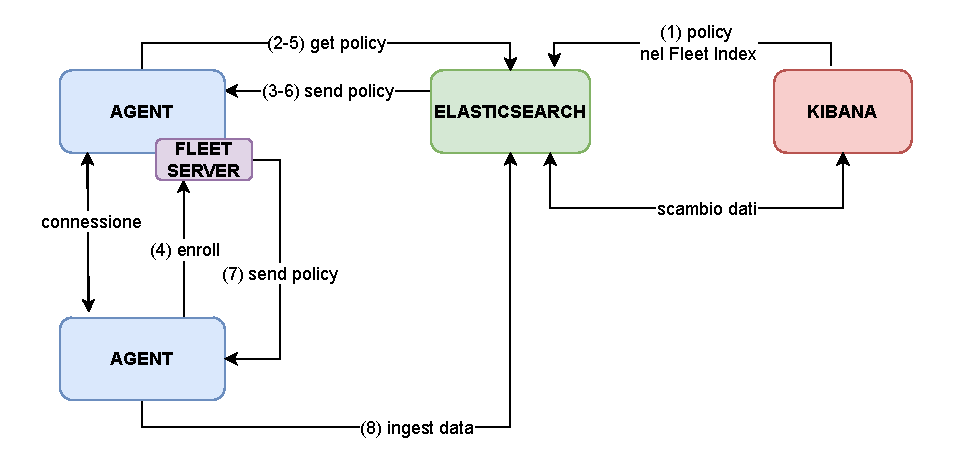
\includegraphics[width=1\linewidth]{images/ECK_flow.drawio.pdf}
	\caption{Diagramma del flusso di funzionamento dello stack}\label{eck flow}
\end{figure}

All'avvio di \emph{Kibana} le policy specificate nella configurazione, avvenuta tramite \emph{helm chart}, vengono salvate in un indice, denominato \emph{Fleet}, all'interno di Elasticsearch. \\
Il \emph{Fleet Server}, all'avvio, stabilisce una connessione tramite i riferimenti posti tra i values con Kibana, per abilitare l'interfaccia grafica di gestione Fleet, e con Elasticsearch per ottenere i dati contenuti nell'indice di Fleet, ovvero le policy definite. In concreto, il Fleet Server funziona come un agente normale, con la differenza che viene ``enrollato'' in una policy server.\\
Gli \emph{Agenti}, all'avvio, essendo \textit{fleet-enrolled} cercheranno di stabilire una connessione con il Fleet Server tramite il riferimento specificato.\@ Andranno a richiedere al server la policy specificata nella loro configurazione (\texttt{policyID: eck-agent}) e Fleet si occuperà di recuperarla dall'indice di Elasticsearch per consegnarla al richiedente legittimo. Si dice quindi terminata la fase di \emph{enrollment}. \\
Aprendo l'interfaccia di Fleet tramite Kibana è quindi possibile gestire le due policy caricate e i relativi agent che sono stati ``enrollati''; le modifiche effettuate tramite il Fleet server alle policy vengono riflesse nell'indice di Elasticsearch e negli agent che seguono quella policy, effettuando un upgrade automatico.
Viene mantenuta una connessione attiva tra agenti e fleet server per controllare lo stato di salute e la disponibilità di aggiornamenti; quando un agente si collega e c'è stato un cambiamento, il Fleet Server recupera da Elasticsearch la policy e la consegna all'agente effettuando così un aggiornamento autonomo. \\
Una volta che l'intera infrastruttura è stata deployata si hanno 3 agenti \emph{fleet-enrolled}, uno per ciascuno nodo, che vanno ad usare le informazioni contenute nella policy per raccogliere i dati e inviarli ad Elasticsearch; gli agenti hanno un'architettura di tipo Push in quanto inviano attivamente i dati ad un endpoint che si occuperà di salvarli in appositi indici.\\
Tramite l'interfaccia di gestione delle policy è possibile scegliere quali Integrazioni aggiungere, andando così a raccogliere dati da una nuova sorgente e causando un rilascio di una nuova versione della rispettiva policy con conseguente aggiornamento degli agent. \\
Oltre a svolgere operazioni di ricerca e analisi tramite la \gls{GUI} di Kibana è possibile inviare query agli endpoint di Elasticsearch, i quali mettono a disposizione una serie di \gls{API} REST\footnote{\url{https://www.elastic.co/guide/en/elasticsearch/reference/current/rest-apis.html}}.

\section{Assurance Engine}
L'applicativo viene sviluppato in Rust\footnote{\url{https://www.rust-lang.org/}}, un linguaggio sicuro e ad alte prestazioni che previene molti errori comuni, fondandosi su 3 pacchetti principali quali Tokio\footnote{\url{https://tokio.rs/}}, per la gestione dell'esecuzione asincrona, Poem\footnote{\url{https://crates.io/crates/poem}}, come framework web, e PoemOpenAPI\footnote{\url{https://crates.io/crates/poem-openapi}}, per l'implementazione automatica di \gls{API} e della relativa documentazione. \\
L'engine sviluppato si basa inoltre sui due concetti principali dell'Assurance Methodology, le \textbf{metriche} e i \textbf{contratti}, visti nella Sezione \ref{assurance methodology} e ora realizzati concretamente sotto forma di \emph{Trait}; un componente Rust che definisce in modo astratto il comportamento/la funzionalità che un particolare tipo ha e può condividere con altri tipi.  \\
La Figura \ref{metriche_contratti} mostra uno schema che, partendo dai dati grezzi, illustra i passaggi chiave da compiere prima di arrivare ad un report del sistema.

\begin{figure}[ht]
	\centering
	
\includegraphics[width=.9\linewidth]{images/ae/metriche-contratti.drawio.pdf}
	\caption{Diagramma del funzionamento}\label{metriche_contratti}
\end{figure}

Le funzionalità sviluppate vengono poi rese accessibili tramite l'esposizione di \textbf{\gls{API} rest} conformate ai criteri di \emph{OpenAPI Specification v3}\footnote{\url{https://github.com/OAI/OpenAPI-Specification/blob/main/versions/3.1.0.md}}; vengono quindi seguite alcune delle linee standard precedentemente identificate nella Sezione \ref{standard}. \\
Segue l'illustrazione dei vari punti chiave nominati.


\subsection{Metric e Measurement}\label{metric trait}
\'E stato definito il trait parametrico \texttt{Metric} come riportato nel Codice \ref{trait metric} che permette di specificare il tipo dell'argomento (\texttt{Arguments}) e dell'\texttt{Output}, i quali devono a loro volta soddisfare determinati \emph{trait bounds} (Send + Sync + \dots). Fornisce quindi un'interfaccia generica che codifica la struttura di una metrica definendo la firma di due metodi, \texttt{description()} e \texttt{measure()}.
Il primo è semplicemente una funzione che ritorna una descrizione letterale della metrica. Il secondo, invece, è il metodo che concretamente va ad ottenere le misurazioni dagli endpoint di monitoring.

\begin{lstlisting}[language=Rust, caption= Metric Trait \label{trait metric}, basicstyle=\ttfamily ]
  #[async_trait]
  pub trait Metric<Arguments, Output>
      where
    Arguments: Send + Sync + Type + ParseFromJSON + ToJSON,
    Output: Send + Sync + Type + ParseFromJSON + ToJSON,
  {
      fn id(&self) -> Box<str> {
          Box::from(std::any::type_name::<Self>())
      }

      fn description(&self) -> Box<str>;

      async fn measure(&self, args: Arguments)
        -> Result<Measurement<Arguments, Output>, Error>;
  }
\end{lstlisting}

L'implementazione concreta, in questo contesto, di quest'ultimo metodo va a costruire ed eseguire le query contro le \gls{API} esposte dal servizio di Elasticsearch (endpoint) per ottenere i dati (\textit{evidence}).
Prende come input un argomento, \textit{args}, del tipo generico da definire, \texttt{Arguments}, ovvero una struttura specifica che contiene tutti gli argomenti necessari a configurare la richiesta, include quindi sia la query vera e propria che dei parametri di configurazione come l'indice di interesse e la dimensione, come rappresentato nel Codice \ref{Arguments struct}.

\begin{lstlisting}[language=Rust, caption= Arguments Struct \label{Arguments struct}, basicstyle=\ttfamily ]
  #[derive(Debug, Clone, PartialEq, serde::Deserialize,
      serde::Serialize, Object)]
  pub struct BasicSearchArgs {
      pub query: Value,
      pub index: Vec<String>,
      pub from: Option<i64>,
      pub size: Option<i64>,
  }
\end{lstlisting}

\subsubsection{Measurement}\label{measurement section}
In output, a meno di errori, il metodo \texttt{measure()} restituisce un \texttt{Measurement}, una struttura che rappresenta il risultato dalla misurazione, costituita dai campi \texttt{time}, \texttt{args} e \texttt{value} come mostrato nel Codice \ref{Measurement struct}.
Rispettivamente contengono l'istante di tempo in cui è avvenuta la misurazione, gli argomenti passati come input (\texttt{args} di tipo \texttt{Arguments}) e i valori ottenuti.

\begin{lstlisting}[language=Rust, caption= Measurement Struct \label{Measurement struct}, basicstyle=\ttfamily ]
  #[derive(Object)]
  pub struct Measurement<Arguments, Output>
      where
    Arguments: Send + Sync + Type + ParseFromJSON + ToJSON,
    Output: Send + Sync + Type + ParseFromJSON + ToJSON,
  {
      /// Time instant of measurement
      pub time: OffsetDateTime,
      /// Arguments in input
      pub args: Arguments,
      /// Value registered
      pub value: Output,
  }
\end{lstlisting}

Qui entra in gioco il secondo parametro di tipo generico da definire, ovvero \texttt{Output}, che definisce la struttura del risultato da andare ad includere all'interno del \texttt{Measurement}, come si può vedere nel Codice \ref{Output struct} si tratta di un solo valore, \texttt{output}, che permette il contenimento di una stringa in formato json.

\begin{lstlisting}[language=Rust, caption= Output Struct \label{Output struct}, basicstyle=\ttfamily ]
  #[derive(Debug, Clone, PartialEq, serde::Deserialize,
      serde::Serialize, Object)]
  pub struct BasicSearchOutput {
      pub output: Value,
  }
\end{lstlisting}

\subsection{Contract ed Evaluation}\label{contract section}
\'E stato definito il trait parametrico \texttt{Contract} come riportato nel Codice \ref{trait contract} che permette di specificare il tipo dell'argomento (\texttt{Arguments}), il quale deve a sua volta soddisfare determinati \textit{trait bounds}. Fornisce quindi un'interfaccia generica che codifica la struttura di un contratto definendo la firma di due metodi, \texttt{description()} e \texttt{evaluate()}. Il primo, come per le metriche, è semplicemente una funzione che ritorna una descrizione letterale. Il secondo, invece, è il metodo che concretamente valuta le misurazioni raccolte combinando strutture di condizioni booleane.

\begin{lstlisting}[language=Rust, caption= Contract Trait \label{trait contract}, basicstyle=\ttfamily ]
  #[async_trait]
  pub trait Contract<Arguments>
      where
    Arguments: Send + Sync + Type + ParseFromJSON + ToJSON,
  {
      fn id(&self) -> Box<str> {
          Box::from(std::any::type_name::<Self>())
      }

      fn description(&self) -> Box<str>;

      async fn evaluate(&self, args: Arguments)
        -> Result<Evaluation<Arguments>, Error>;
  }
\end{lstlisting}

L'implementazione concreta, in questo contesto, di quest'ultimo metodo va ad eseguire il metodo \texttt{measure()}, definito con l'implementazione del \emph{trait metric} visto sopra, e a svolgere dei controlli sulle \emph{misurazioni} che ottiene andando a verificare il superamento o meno di specifiche valutazioni, restituendo un valore booleano che ne definisce l'esito finale.
Prende come input un argomento, \texttt{args}, del tipo generico da definire,
\texttt{Arguments}, ovvero una struttura specifica i cui campi contengono dei valori di riferimento da confrontare con i valori delle misurazioni, per valutare il soddisfacimento o meno del contratto. Si potrebbero impostare, per esempio, dei valori che si desiderano di temperatura minimi, medi e massimi per poi controllare se le misurazioni ottenute rispettano i criteri specificati.
Nel Codice \ref{argument contract struct} viene rappresentata la ''struttura tipo''.

\begin{lstlisting}[language=Rust, caption= Argument Contract Struct\label{argument contract struct}, basicstyle=\ttfamily ]
  #[derive(Debug, Clone, PartialEq, Serialize,
     Deserialize, Object)]
  pub struct SearchContractArgs {
    //values to check the fields with
  }
\end{lstlisting}

\subsubsection{Evaluation}\label{evaluation section}
In output, a meno di errori, il metodo \texttt{evaluate} restituisce un \texttt{Evaluation}, una struttura che rappresenta il risultato della valutazione, costituita dai campi \texttt{time}, \texttt{args} e \texttt{value} come mostrato nel Codice \ref{Evaluation struct}. Rispettivamente contengono l'istante di tempo in cui è avvenuta la misurazione, gli argomenti passati come input (\textit{args} di tipo \texttt{Arguments}) e il valore booleano ottenuto.

\begin{lstlisting}[language=Rust, caption= Evaluation Struct \label{Evaluation struct}, basicstyle=\ttfamily ]
  #[derive(Debug, Clone, PartialEq, Serialize, Deserialize)]
  pub struct Evaluation<Arguments>
      where
    Arguments: Send + Sync + Type + ParseFromJSON + ToJSON,
  {
      /// Time entry in input
      pub time: OffsetDateTime,
      /// Arguments in input
      pub args: Arguments,
      /// Value verified as valid
      pub value: bool,
  }
\end{lstlisting}

\subsection{API}
Come accennato prima le \gls{API} vengono implementate attraverso il crate PoemOpenAPI, il quale garantisce che se il codice compila correttamente allora è pienamente conforme alle Specifiche di OpenAPI v3.
Ogni funzionalità sviluppata, ovvero i metodi \texttt{measure()} per le Metriche ed \texttt{evaluate()} per i Contratti, viene mappata in uno specifico endpoint con il relativo \gls{URL}. Quando viene inviata una richiesta HTTP al \emph{path} configurato, il server esegue la funzionalità corrispondente e restituisce l'esito.
Per ogni funzionalità sviluppata, vengono esposti due endpoint.
Il primo serve a gestire le richieste \emph{POST} consentendo quindi l'esecuzione della funzionalità e l'ottenimento dei risultati; in concreto si tratta dell'effettiva esecuzione del metodo \texttt{measure()} (\ref{trait metric}) o \texttt{evaluate()} (\ref{trait contract}) definito. Il secondo, invece, serve per gestire le richieste \emph{OPTIONS} fornendo una descrizione della funzionalità offerta dall'endpoint; in concreto esegue il metodo \texttt{description()} definito nella rispettiva implementazione.  \\
Poem-OpenAPI permette quindi di associare un \emph{path} e un \emph{method} (POST/OPTIONS) ad una funzione codificata. \\
I risultati, contenuti nelle strutture Measurement \ref{Measurement struct} ed Evaluation \ref{Evaluation struct}, vengono convertiti nelle enumerazioni \texttt{MeasureResponse} ed \texttt{EvaluationResponse} così da ritornare i risultati codificati in formato JSON se tutto è andato a buon fine (\textit{status 200}) oppure, sempre in formato JSON, ritornare il tipo di errore (\textit{400 input error; 500 system error}). \\
Per quanto concerne la \textbf{documentazione} delle API, necessaria per consentire agli utenti di interfacciarsi con esse, viene \emph{generata automaticamente} dalla libreria in conformità allo standard di OpenAPI.
Partendo dalla definizione delle funzioni delle \gls{API}, PoemOpenAPI va a generare un file JSON contenente tutti i dettagli (la documentazione) e lo rende  disponibile tramite uno specifico endpoint, modalità standard di esposizione della documentazione, evitando così la necessità di realizzarla manualmente.


\subsubsection{Swagger UI}
Viene integrata anche una pagina di gestione delle \gls{API} generata automaticamente dalle specifiche OpenAPI, Swagger UI\footnote{\url{https://swagger.io/tools/swagger-ui/}}.
Uno strumento open-source che permette di visualizzare e interagire con le \gls{API} esposte direttamente dal browser attraverso un'interfaccia grafica, che consente di esplorarle e testarle facilmente senza necessità di scrivere codice.
La Figura \ref{swagger ui options/post} mostra l'interfaccia grafica auto-generata da Swagger contenente tutte le \gls{API} esposte, indicando metodo, \textit{path} e una breve descrizione.

\begin{figure}[htb]
	\centering
	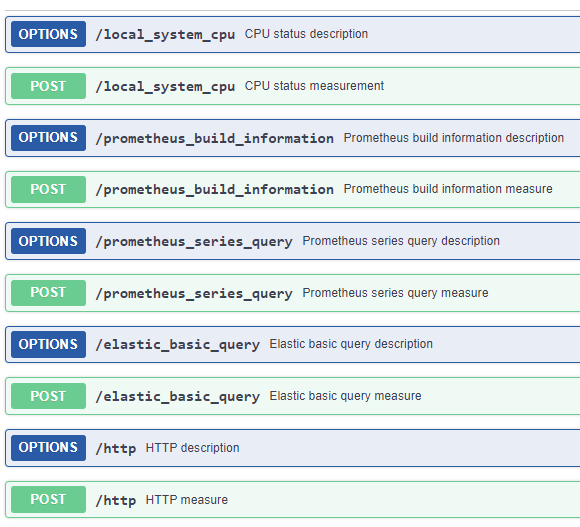
\includegraphics[width=.8\linewidth]{images/swagger/swagger_UI_API.png}
	\caption[Interfaccia di Swagger API esposte]{Interfaccia di Swagger contenente tutte le \gls{API} esposte }\label{swagger ui options/post}
\end{figure}

Andando ad interagire con l'interfacci proposta è possibile, tramite il menù a tendina, espandere la singola \gls{API} vedendone i relativi dettagli.
La Figura \ref{swagger ui post} mostra come deve essere costruito il body di una richiesta di quel tipo, andando a fornire un esempio di valori per quello specifico Schema.
Tramite il bottone ``\textit{Try it out}'' è possibile inviare una richiesta personalizzata su quello specifico endpoint.

\begin{figure}[htb]
	\centering
	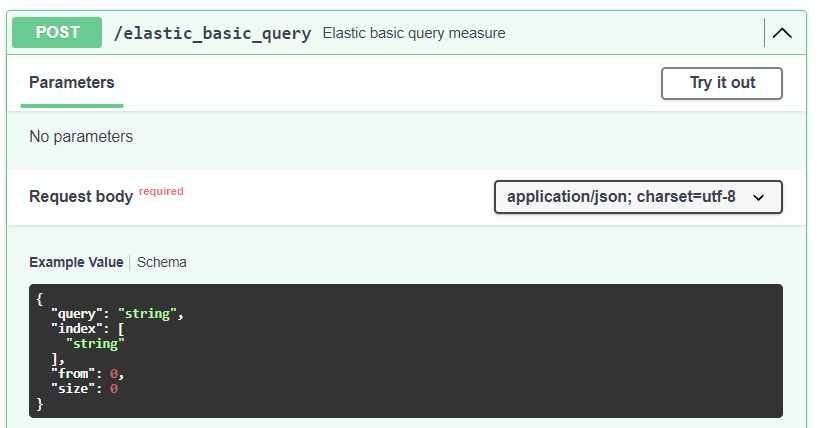
\includegraphics[width=.8\linewidth,]{images/swagger/swagger_UI_post.png}
	\caption[Interfaccia di Swagger esempio richieste POST]{Interfaccia di Swagger contenente un esempio di schema per richieste Post }\label{swagger ui post}
\end{figure}

Si possono ottenere maggiori dettagli riguardo la struttura consultando la sezione Schema, come mostrato nella Figura~\ref{swagger ui schema}, che fornisce anche il tipo associato ai campi.

\begin{figure}[htb]
	\centering
	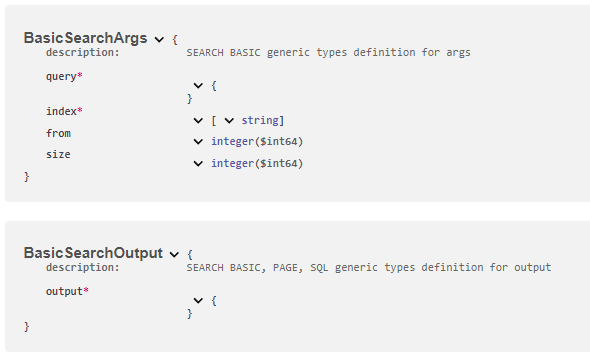
\includegraphics[width=.8\linewidth]{images/swagger/swagger_UI_schema.png}
	\caption[Interfaccia di Swagger schema json con i tipi associati ai valori]{Interfaccia di Swagger contenente lo schema json con i tipi dei valori}\label{swagger ui schema}
\end{figure}


La Figura \ref{swagger ui post response} mostra invece le possibili risposte, con i relativi \textit{status code}, che si possono ottenere inviando una richiesta su uno specifico endpoint; viene anche qui specificato lo schema della risposta in formato JSON.

\begin{figure}[htb]
	\centering
	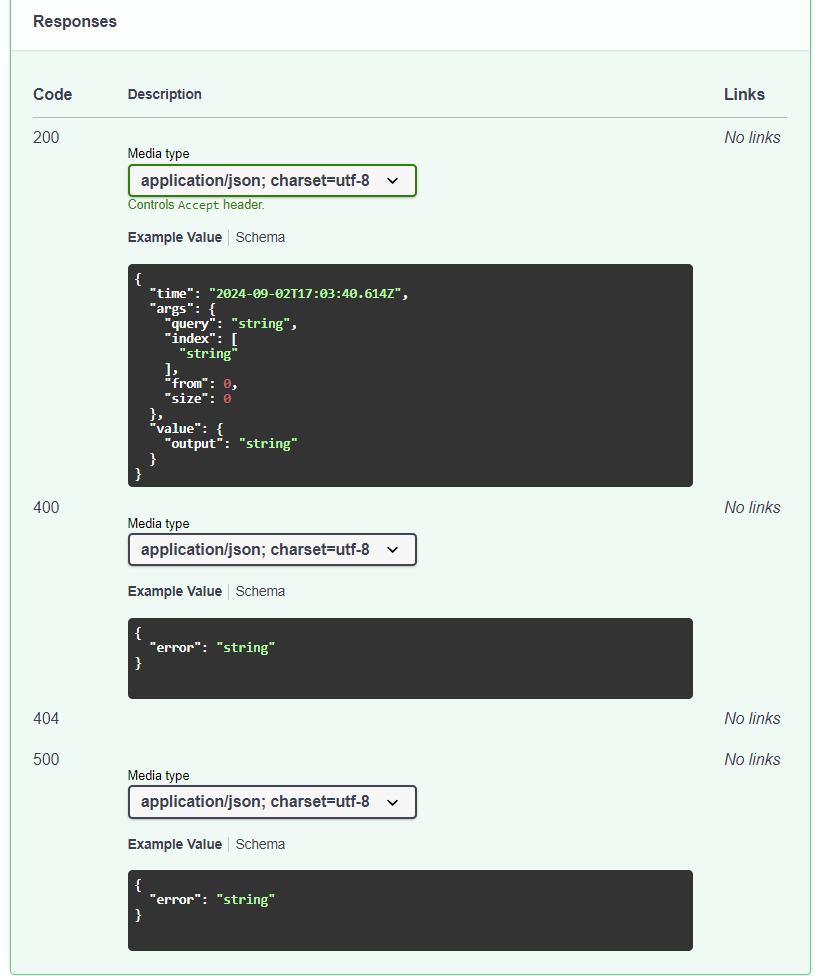
\includegraphics[width=.8\linewidth]{images/swagger/swagger_UI_response.png}
	\caption[Interfaccia di Swagger schema risposte POST]{Interfaccia di Swagger contenente lo schema delle risposte alle richieste POST}\label{swagger ui post response}
\end{figure}


\subsection{Deployment e Vantaggi}\label{vantaggi scal rep}
L'\textit{Assurance Engine} è stato progettato per essere eseguito all'interno di un cluster kubernetes, sfruttando la containerizzazione per garantire una distribuzione semplice e flessibile.
In particolare, l'applicazione viene impacchettata in un container Docker (docker image) minimale contenente il binario eseguibile dell'engine che successivamente viene deployato all'interno del cluster Kubernetes.
Una volta in esecuzione all'interno del cluster, l'applicativo cercherà di collegarsi agli altri servizi integrati nell'engine e disponibili all'interno dell'ecosistema, come Elasticsearch o Prometheus ad esempio. \\
Il sistema, per come è strutturato, si pone da \emph{intermediario} tra l'utente finale e alcuni servizi di monitoring facendo in modo di ricevere le richieste dall'utente e successivamente indirizzarle all'apposito servizio. Questa infrastruttura può essere vista in un certo senso come un \textit{request-reflector} che però, adottando questo design di sviluppo, fornisce svariati vantaggi tra cui la garanzia di alcune proprietà chiave per l'Assurance Engine, come la \emph{scalabilità}, la \emph{replicabilità} e l'\emph{assenza di coordinazione aggiuntiva} in ambienti distribuiti.

\paragraph{Scalabilità e Replicabilità}
Queste importanti proprietà, derivanti dalla struttura dell'applicazione, consentono di deployare l'engine come una singola istanza o come istanze multiple, permettendo quindi di scegliere il numero di \emph{repliche deployabili} per rendere il sistema distribuito. \\
L'architettura, pur essendo distribuita, non necessita alcuna coordinazione aggiuntiva tra le varie istanze/repliche in quanto tutte \emph{equivalenti e intercambiabili} tra loro: le richieste possono essere inviate indistintamente a una qualsiasi istanza disponibile e verranno risolte in modo identico. Un \emph{network load balancer}, come un \emph{kubernetes service}, si occuperà di distribuire il traffico, in base alle condizioni della rete, tra le varie repliche disponibili.
Questa semplicità è possibile perché il compito che ogni replica assolve è quello di intermediario \textit{stateless} verso servizi di backend come Elasticsearch. \\
La Figura \ref{assurance engine deployment} mostra uno schema di un semplice cluster in cui sono state deployate 3 repliche dell'Assurance Engine poste dietro ad un network load balancer.
Indipendentemente dalla replica a cui la richiesta verrà inoltrata dal load balancer, esse arriveranno sempre allo stesso servizio di backend.

\begin{figure}[h!]
	\centering
	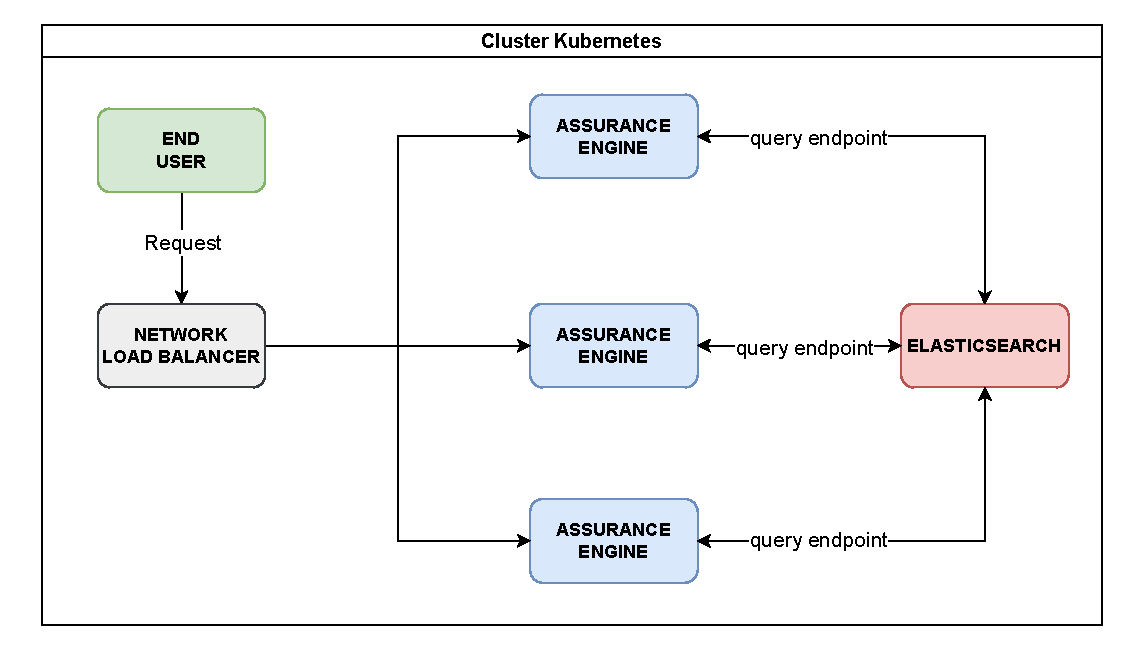
\includegraphics[width=.9\linewidth]{images/ae/AssuranceEngine.drawio.pdf}
	\caption{Diagramma Assurance Engine deployato su 3 nodi}\label{assurance engine deployment}
\end{figure}

\subsubsection{Necessità di questo ''framework intermediario''}
Lo scopo di un sistema di assurance è garantire il soddisfacimento di determinate proprietà da parte di un sistema target. \\
La domanda che viene spontaneo porsi è quindi:
\textit{Come mai, essendo che Elasticsearch fornisce analisi per informazioni provenienti da una moltitudine di entità diverse, si è ricorsi ad un layer aggiuntivo (assurance engine), posto tra l'utente e il servizio di backend, per svolgere controlli di assurance?} \\
La risposta a questa domanda si trova nella definizione di sistema di assurance posta qua sopra; un sistema di assurance è quanto più completo e generico quante più proprietà e sistemi target eterogenei riesce a verificare. \\
Aggiungendo questo strato di interfacciamento è stato possibile accaparrarsi tutti i \textbf{vantaggi di Elasticsearch}, come la possibilità di collezionare dati da una moltitudine di servizi eterogenei grazie alle specifiche \textit{Integration} e l'\textit{efficienza} nel salvataggio e nella ricerca dei dati in un sistema distribuito.
A questi, vanno ad aggiungersi i \emph{vantaggi architetturali dell'assurance engine} illustrati nella Sezione precedente \ref{vantaggi scal rep}, che garantiscono \textbf{scalabilità} e \textbf{replicabilità}.
Infine, il punto chiave che giustifica questo strato, si riconduce alle potenzialità che vengono offerte dall'utilizzo di un \textbf{linguaggio di programmazione} efficiente e affidabile come Rust.
Utilizzando un vero e proprio linguaggio di programmazione invece che il limitato linguaggio di scripting \textit{built-in} di Elasticsearch, è possibile avere una potenza espressiva maggiore sia per fare controlli più complessi (contratti) che per ottenere dati in modalità non implementate nei servizi di backend (\textit{probe custom}). Alcuni esempi sono l'invio di semplici richieste HTTP verso un sito web per verificarne l'availability oppure l'invio di payload specifici su determinati endpoint per monitorarne la reazione; questo tipo di attività, possibile grazie all'impiego di un linguaggio di programmazione, permette quindi di analizzare contesti più generici.
I servizi come Elasticsearch, invece, non consentono l'invio di richieste avanzate o \textit{taylor-made} verso target specifici; il servizio recupera delle metriche dal target ma non ha una parte di ''\textit{probe custom}'' che gli permette di ottenere informazioni specifiche. \\
In conclusione il vantaggio si piò riassumere in una parola \textbf{genericità}, si possono combinare informazioni da varie entità diverse.


\subsection{Funzionamento}\label{funzionamento ae}
Viene illustrato un esempio di ciclo completo di funzionamento.
La Figura \ref{assurance engine flow} mostra un'automa a stati finiti contenente lo schema del funzionamento illustrato tramite componenti grafici.

\begin{figure}[ht!]
	\centering
	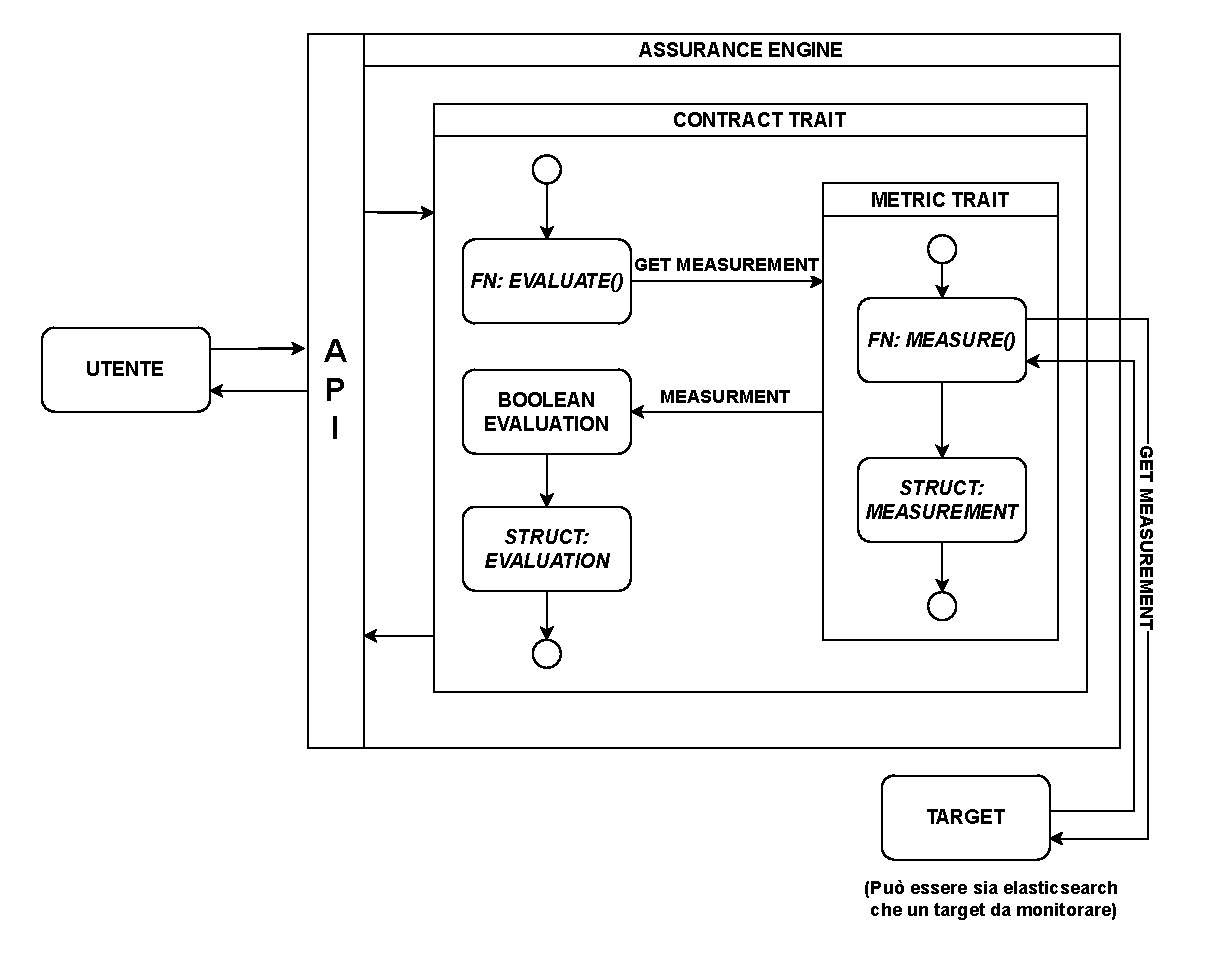
\includegraphics[width=.9\linewidth]{images/ae/Assurance_engine_flow.drawio.pdf}
	\caption{Assurance Engine: Flusso di esecuzione}\label{assurance engine flow}
\end{figure}

La prima operazione inizia dall'utente che invia una richiesta ad un endpoint esposto dal'\textit{Assurance Engine}, supponiamo per completezza il metodo POST di un contratto.
Il server, quando riceve la richiesta, va ad eseguire il metodo \texttt{evaluate()} definito per quella funzionalità. L'esecuzione può essere suddivisa concettualmente nelle 3 parti focali precedentemente definite nell'\emph{Assurance Process} definito nella Sezione \ref{assurance process}; rispettivamente sono \emph{Measurement collection}, \emph{Contract evaluation} e {Report composition}.

\paragraph{Measurement collection}
In questa fase viene eseguito il metodo \texttt{measure()} precedentemente illustrato nella Sezione \ref{metric trait} che si occupa di ottenere delle metriche da un target. Come accennato prima, grazie alla genericità di cui gode, il metodo \texttt{measure()} può andare ad interrogare un servizio di backend come Elasticsearch o inviare richieste custom.
I dati ottenuti vengono trattati come \texttt{measurements} e di fatto costituiscono le \textit{evidence} o prove necessarie ai contratti per stilare una valutazione del sistema; seguono il modello definito nella Sezione \ref{measurement section}.
Viene effettuata quindi una fase di parsing della risposta JSON ottenuta all'interno del \textit{measurement} andando ad estrarre i campi e i valori desiderati; vengono svolte anche operazioni di aggregazione dei dati come somme, medie, ecc (\emph{metric evaluation}).
Una volta ottenute le evidence definitive inizia la seconda fase.

\paragraph{Contract evaluation}
Questa fase è concettualmente molto semplice ma racchiude al suo interno la potenzialità e le garanzie che questo sistema può offrire. Si tratta di controlli booleani effettuati tra le \emph{measurements} ottenute facendo \emph{metric evaluation} e gli argomenti passati come parametri al contratto, precedentemente visti nella Sezione \ref{contract section} alla Figura \ref{argument contract struct}.
I risultati dei vari controlli singoli sulle metriche vengono successivamente aggregati in un'unico risultato finale che dichiara il soddisfacimento o meno della proprietà che si stava verificando.

\paragraph{Report composition}
L'ultima fase si tratta semplicemente di ritornare i risultati ottenuti in modo formale e valutabile a posteriori. Viene quindi ritornata la struttura definita nella Sezione \ref{evaluation section} contenente sia l'esito che gli argomenti usati per fare la valutazione, in aggiunta al \textit{timestamp}.

L'utente che ha inviato la richiesta riceve una risposta in formato JSON, contenente o la struttura sopra definita oppure una descrizione della tipologia dell'errore che è incorso.


\subsection{Esempi di richieste: Elastic e SQL Query}
Di seguito vengono proposti tre esempi di utilizzo del metodo \texttt{measure()}, per raccogliere metriche da Elasticsearch, con tre query differenti in formato JSON. Le prime due sfruttano il linguaggio di ricerca fornito da Elasticsearch, un completo Query \gls{DSL} basato su JSON, mentre la seconda permette di effettuare ricerche usando query SQL e ritornando i risultati in forma tabellare. \\
L'ultimo esempio mostra uno schema generale di invocazione del metodo \texttt{measure()} con una generica query.

\begin{exmp}
	Esempio di ricerca che colleziona \textbf{tutti i dati} presenti nell'indice e li ordina cronologicamente sulla base dei campi Date e Time del dataset. Di seguito, nel Codice \ref{JSON query all}, viene mostrata la query in formato JSON necessaria per svolgere tale operazione.

	\begin{lstlisting}[language=json, caption=Valori JSON per query \emph{match all} \label{JSON query all}, basicstyle=\ttfamily]
  "query": {
      "match_all": {}
      },
  "sort": [
      {"Date": {"order" : "asc"}},
      {"Time": {"order" : "asc"}}
  ],
  \end{lstlisting}
\end{exmp}

\begin{exmp}
	Esempio di ricerca che colleziona i dati presenti nell'indice il cui \textbf{intervallo temporale}, campi Date e Time, rispetta un certo criterio e li ordina cronologicamente. Di seguito, nel Codice \ref{JSON query range}, viene mostrata la query in formato JSON necessaria per svolgere tale operazione.

	\begin{lstlisting}[language=json, caption= Valori JSON per query \emph{range} su intervalli temporali \label{JSON query range}, basicstyle=\ttfamily]
  "query": {
    "range": {
        "Date": {
            "gte": "11/03/2004",
            "lte": "15/03/2004"
        },
        "Time": {
            "gte": "18.00.00",
            "lte": "24.00.00"
        }
    }
  },
  "sort": [
      {"Date": {"order" : "asc"}},
      {"Time": {"order" : "asc"}}
  ],
  \end{lstlisting}
\end{exmp}

\begin{exmp}
	Esempio di ricerca eseguito tramite query \textbf{SQL} che estrae due campi dall'indice filtrando per il campo Date. Nel Codice \ref{JSON query sql}, viene mostrata la query in formato JSON necessaria per svolgere tale operazione.

	\begin{lstlisting}[language=json, caption= Valori JSON per query \emph{SQL} \label{JSON query sql}, basicstyle=\ttfamily]
    "query": "SELECT T, \"NO2(GT)\"
              FROM imported_dataset
              WHERE Date = '05/10/2004'"
  \end{lstlisting}
\end{exmp}


\begin{exmp}
	Nel seguente Codice \ref{rust query} viene mostrata l'invocazione del metodo \texttt{measure()} con la relativa generica query specificabile tramite valori JSON nel Query \gls{DSL} di Elastic.

	\begin{lstlisting}[language=rust, caption= Esecuzione Rust della query nel linguaggio di Elastic\label{rust query}, basicstyle=\ttfamily]
  client.measure(BasicSearchArgs {
      query: json!({<json_values>}),
      index: vec!["imported_dataset".to_string()],
      from: None,
      // size: Some(1)
      size: None,
  })
  \end{lstlisting}

	Mentre in questo Codice \ref{rust query sql} viene mostrata l'invocazione del metodo \texttt{measure()} con la relativa generica query SQL specificabile tramite valori JSON.
	\begin{lstlisting}[language=rust, caption= Esecuzione Rust della query SQL \label{rust query sql}, basicstyle=\ttfamily]
  client.measure(ArgsSQL {
    query: json!({<json_values>})
  })
  \end{lstlisting}
\end{exmp}

% OPTIONAL TODO
%\subsection{Dettagli extra - opzionale}
%%+ forse dettagli tokio o in una subsection
%\hl{
%	Dettagli implementativi extra: \\
%	-ambiente asincrono (tokio) che distribuisce il carico (valutazione %metriche, contratti, ecc) in modo efficacemente su più core (asincrono %run time work stealing, scala bene su più core)\\
%}

\chapter{Esperimenti}\label{esperimenti}
In questo capitolo verranno presentati i test condotti sulle performance del sistema di \emph{Assurance Engine} collegato ad Elasticsearch.
L'obiettivo è quello di descrivere i tipi di test/benchmark eseguiti e i risultati oggettivi ottenuti tramite grafici e tabelle riepilogative.
Questi benchmark sono stati selezionati perché rappresentano i principali casi d'uso nel contesto di misurazione e valutazione delle performance.
In altre parole, sono stati analizzati quegli aspetti statistici chiave, cruciali per comprendere e ottimizzare le prestazioni complessive del sistema.
I benchmark sono stati condotti utilizzando Criterion\footnote{\url{https://bheisler.github.io/criterion.rs/book/}}, una libreria di benchmarking utilizzata per misurare e analizzare prestazioni di esecuzione di specifiche funzioni per il linguaggio di programmazione Rust.

%%%%%%%%%%%%%%%%%%%%%%%%%%%%%%%%%%%%%%%%%%%%%%%%%%%%%%%%%%%%
%%%%%%%%%%%%%%%%%%%%%%%%%%%%%%%%%%%%%%%%%%%%%%%%%%%%%%%%%%%%
\section{Statistiche offerte}
L'implementazione di benchmark tramite Criterion fornisce delle tabelle, denominate \textit{additional statistics}, e dei diagrammi per poter analizzare e confrontare i risultati ottenuti.
Vengono elencate di seguito tutte le \textit{additional statistics} ottenibili con una breve illustrazione. \'E da considerare che tutte le valutazioni vengono espresse tramite intervalli di confidenza, seguono quindi la forma \texttt{[<lower bound> <estimated>  <upper bound>]}.
%https://bheisler.github.io/criterion.rs/book/user_guide/command_line_output.html#additional-statistics
\begin{itemize}
	\item \textbf{R2} Coefficiente di Determinazione. \'E una misura della bontà di adattamento di un modello di regressione lineare ai dati; misura quindi la correttezza del modello statistico utilizzato. Se il valore R2 è basso, questo potrebbe indicare che il benchmark non sta eseguendo la stessa quantità di lavoro a ogni iterazione.

	\item \textbf{Mean} Media dei tempi per iterazione
	\item \textbf{Std. Dev.} Deviazione Standard dei tempi per iterazione. \'E una misura della dispersione o variabilità di un insieme di dati che indica quanto i valori di un dataset si discostano in media dalla loro media aritmetica. \\
	      Se è più grande rispetto agli altri valori di tempo significa che i benchmark sono rumorosi e potrebbe essere necessario modificarli per ridurre il rumore.

	\item \textbf{Median} Mediana. \'E una misura che indica il valore centrale di una distribuzione; divide un dataset ordinato in due metà uguali contenenti lo stesso numero di valori (o quasi).
	\item \textbf{\gls{MAD}} Deviazione Assoluta Mediana. \'E una misura di dispersione che quantifica quanto i dati si discostano dalla loro mediana. \'E un'alternativa alla deviazione standard e viene utilizzata per misurare la variabilità dei dati in modo che sia meno influenzata dai valori estremi o outliers. \\
	      Se la deviazione assoluta mediana è ampia indica che i parametri di riferimento sono rumorosi.

	\item \textbf{Outliers} Valori anomali. Vengono rilevate misurazioni insolitamente sproporzionate rispetto alle restanti, sia valori troppo alti che troppo bassi. \\
	      Se sono presenti molti valori anomali, la misurazione ci suggerisce che i risultati del benchmark sono rumorosi e non pienamente affidabili.
\end{itemize}


Oltre ai dati presentati in forma tabellare (ed immagazzinati in formato JSON), Criterion mette a disposizione vari diagrammi o \textit{plot} per rappresentare graficamente le performance.

\begin{itemize}
	\item \textbf{Violin plot} Diagramma a violino. Una rappresentazione statistica che descrive distribuzioni di probabilità utilizzando curve di densità; viene utilizzato per confrontare distribuzioni e quindi confrontare i benchmark.
	\item \textbf{Density plot} Diagramma della densità. Mostra il tempo medio per iterazione. Nel diagramma si ha una regione colorata che rappresenta la probabilità che un iterazione richieda quella quantità di tempo e una linea marcata che identifica la media.
	\item \textbf{Time/Iteration plot} Mostra il tempo medio di iterazione impiegato dai diversi sample o tentativi. Ogni tentativo (generalmente da 0 a 100) viene rappresentato da un puntino e l'altezza ne definisce il tempo utilizzato.
\end{itemize}

%%%%%%%%%%%%%%%%%%%%%%%%%%%%%%%%%%%%%%%%%%%%%%%%%%%%%%%%%%%%
%%%%%%%%%%%%%%%%%%%%%%%%%%%%%%%%%%%%%%%%%%%%%%%%%%%%%%%%%%%%
\section{Benchmark}
I benchmark scritti utilizzando il framework Criterion vengono eseguiti tramite il comando \texttt{cargo bench -p ae-probes --bench elastic\_probes}.
L'esecuzione di ogni benchmark viene suddivisa in quattro fasi.
\begin{enumerate}
	\item \textit{\textbf{Warm-up}}: la funzione sottoposta al benchmark viene eseguita ripetutamente per un periodo di tempo configurabile, di default 3 secondi.
	      Serve a riscaldare le cache del processore e (se applicabile) le cache del file system per adattarsi al nuovo carico di lavoro.

	\item \textit{\textbf{Measurement}}: la funzione sottoposta al benchmark viene eseguita ripetutamente per generare una stima del tempo impiegato da ogni iterazione; ogni iterazione viene definite come un sample e contiene le rispettive misurazioni.

	\item \textit{\textbf{Analysis}}: i sample vengono analizzati per calcolare le statistiche che vengono riportate, salvate e disegnate.

	\item \textit{\textbf{Comparison}}: il sample corrente viene confrontato con il sample ottenuto nell'iterazione del benchmark precedente.
\end{enumerate}

Terminate queste fasi e quindi terminato il benchmark viene generata una struttura di directory all'interno del progetto Rust sotto \textit{assurance-engine/target/criterion/<BENCHMARK\_NAME>} come mostrato nella Figura \ref{benchmark directory}.

\begin{figure}
	\centering
	\begin{subfigure}{\textwidth}
		\dirtree{%
			.1 \textbf{BENCHMARK\_NAME/}.
			.2 \textbf{base/}.
			.3 benchmark.json.
			.3 estimates.json.
			.3 sample.json.
			.3 tukey.json.
			.2 \textbf{change/}.
			.3 estimates.json.
			.2 \textbf{new/}.
			.3 benchmark.json.
			.3 estimates.json.
			.3 sample.json.
			.3 tukey.json.
			.2 \textbf{report/}.
			.3 both/.
			.4 pdf.svg.
			.4 iteration\_times.svg.
			.4 regression.svg (optional -> not present).
			.3 change/.
			.4 mean.svg.
			.4 median.svg.
			.4 t-test.svg.
			.3 index.html.
			.3 MAD.svg.
			.3 mean.svg.
			.3 median.svg.
			.3 SD.svg.
			.3 slope.svg (optional -> not present).
			.3 pdf.svg.
			.3 pdf\_small.svg.
			.3 relative\_pdf\_small.svg.
			.3 iteration\_times.svg (optional -> present).
			.3 iteration\_times\_small.svg (optional -> present).
			.3 relative\_iteration\_times\_small.svg (optional -> present).
			.3 regression.svg (optional -> not present).
			.3 regression\_small.svg (optional -> not present).
			.3 relative\_regression\_small.svg (optional -> not present).
		}
	\end{subfigure}
	\caption{Directory tree generato dai benchmark di Criterion}\label{benchmark directory}
\end{figure}

La cartella \textit{/new} contiene le statistiche dell'ultimo benchmark eseguito mentre la cartella \textit{/base} include le statistiche del benchmark precedente oppure è rimpiazzata da cartelle con il nome dei benchmark salvati.
Tramite il comando \texttt{cargo bench -\phantom{}-bench elastic\_probes -\phantom{}- -\phantom{}-save-baseline <nome>} è possibile andare a salvare un benchmark con un nome e
tramite il comando \texttt{cargo bench -\phantom{}-bench elastic\_probes -\phantom{}-baseline <nome>} è possibile selezionarlo come benchmark per il confronto. \'E stato salvato un benchmark eseguito localmente nel laboratorio.\\
Il comando utilizzato per ottenere le statistiche dettagliate delle valutazioni in locale e confrontarle graficamente coon le altre salvate precedentemente è il seguente: \texttt{cargo bench -p ae-elastic-probe -\phantom{}-bench elastic\_probes -\phantom{}- -\phantom{}-load-baseline locale -\phantom{}-baseline old}. \\
La cartella \textit{/report} contiene tutti i diagrammi, sia quelli generati del singolo benchmark che quelli del confronto con uno precedente, contenuti nella sotto-cartella \textit{/both}.
I risultati tramite interfaccia grafica sono consultabili aprendo il file \textit{/report/index.html}.

Il benchmark effettuato valuta concretamente l'esecuzione di 4 funzione suddivise a coppie. Le prime due utilizzano la ricerca tramite Query \gls{DSL} proposta nel Codice \ref{JSON query all} che estrae tutti gli elementi e li ordina cronologicamente. Le altre due, invece, utilizzano la ricerca tramite query SQL proposta nel Codice \ref{JSON query sql} che estrae due campi dall'indice filtrando sulla data. Ogni coppia è costituita da una funzione \texttt{measure()} per le Metriche e da una funzione \texttt{evaluate()} per i Contratti. \\
Di seguito, per ogni tipo di ricerca (SEARCH e SQL), viene proposto prima un confronto tra l'esecuzione dei due metodi, \texttt{measure} ed \texttt{evaluate}, tramite un diagramma a violino e poi un'analisi dettagliata dei metodi presi singolarmente.

%%%%%%%%%%%%%%%%%%%%%%%%%%%%%%%%%%%%%%%%%%%%%%%%%%%%%%%%%%%%
%%%%%%%%%%%%%%%%%%%%%%%%%%%%%%%%%%%%%%%%%%%%%%%%%%%%%%%%%%%%
\section{SEARCH Benchmark}
Benchmark effettuato sulle funzioni \texttt{measure()} ed \texttt{evaluate()} basate sulla Query \gls{DSL} proposta nel Codice \ref{JSON query all} che estrae tutti gli elementi e li ordina cronologicamente.

\paragraph{Confronto funzioni benchate}
La Figura \ref{violino search} mostra due distribuzioni di probabilità indicanti il tempo medio di esecuzione delle funzioni \texttt{evaluate} e \texttt{measure}.
L'asse delle ascisse rappresenta il tempo di esecuzione, mentre quello delle ordinate i due benchmark da confrontare.
Si osserva come le distribuzioni si concentrino introno al valore medio, 6 ms per le metriche e 5 ms per i contratti. 
Tuttavia, si nota come l'ampiezza del benchmark di Metric si discosti notevolmente dal valore medio a causa di alcuni \textit{outliers} misurati, sopra i 9 ms; sono identificati da una riga orizzontale che quindi ne definisce una probabilità trascurabile.
In conclusione, l'esecuzione del benchmark sui contratti è stata omogenea in quanto tutte le misurazioni hanno ottenuto valori addensati intorno ai 5 ms. Nel caso dei benchmark sulle metriche, invece, si nota una media spostata leggermente verso destra, 6 ms, poiché influenzata da misurazioni outliers.

\begin{figure}[h]
	\centering
	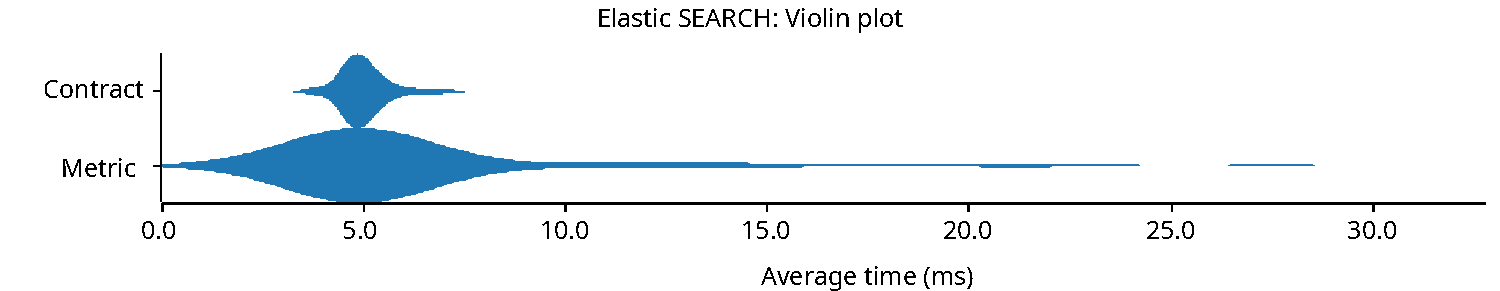
\includegraphics[width=1\linewidth]{images/benchmark/SEARCH/search-violin.pdf}
	\caption{Diagramma a violino richieste di tipo SEARCH}\label{violino search}
\end{figure}
%%%%%%%%%%%%%%%%%%%%%%%%%%%%%%%%%%%%%%%%%%%%%%%%%%%%%%%%%%%%
%%%%%%%%%%%%%%%%%%%%%%%%%%%%%%%%%%%%%%%%%%%%%%%%%%%%%%%%%%%%
\subsection{Metric - \texttt{measure()}}\label{section metric search}
\paragraph{Diagramma distribuzione probabilità-tempo}
La Figura \ref{densità metric search} illustra la distribuzione di probabilità relativa al tempo necessario per eseguire il metodo \texttt{measure}. Si possono osservare quattro picchi nel diagramma. 
Il primo, nonché più significativo, determina prevalentemente il comportamento di questa distribuzione, in quanto possiede l'altezza massima e quindi una densità di probabilità maggiore; il picco si trova sul valore 5 ms.
Gli altri altri 3 picchi identificati sono di rilevanza inferiore più ci si allontana dal valore del picco massimo. 
Questi ultimi si trovano oltre al valore definito come limite massimo per decretare un valore conforme agli altri e quindi non outlier; nel diagramma viene rappresentato da una linea rossa a 9 ms, ``severe outliers''. Gli outlier sono identificati da puntini rossi mentre la media è rappresentata da una linea blu a a 6.2 ms.
\begin{figure}[h]
	\centering
	
\includegraphics[width=1\linewidth]{images/benchmark/SEARCH/metric/density.pdf}
	\caption{Diagramma densità probabilistica richieste \texttt{measure} di tipo SEARCH}\label{densità metric search}
\end{figure}

\paragraph{Statistiche calcolate}
Nella Tabella \ref{benchmark search metric} vengono mostrate le statistiche ottenute tramite i benchmark. Si nota una media del tempo di esecuzione pari a 6.2 ms e una deviazione standard rispetto tale valore pari a 4.1 ms.
\begin{table}[h]
	\caption{Valutazioni statistiche SEARCH/Metric benchmark}\label{benchmark search metric}
	\centering
	\begin{tabularx} {0.9\textwidth}
		{C| c*{3}{C}} % C è un column type definito nel main
		\toprule
		\textbf{Misurazione} & \textit{Lower bound} & \textbf{Estimate}  & \textit{Upper bound} \\

		\midrule
		\textbf{Mean}        & 5.5126 ms            & \textbf{6.2485 ms} & 7.1098 ms            \\
		\textbf{Std. Dev.}   & 2.5683 ms            & \textbf{4.1361ms}  & 5.4378 ms            \\
		\textbf{Median}      & 4.8315 ms            & \textbf{5.0052 ms} & 5.1727 ms            \\
		\textbf{\gls{MAD}}   & 691.05 µs            & \textbf{906.15 µs} & 1.0739 ms            \\
		\textbf{R2}          & 0.0005357            & \textbf{0.0005529} & 0.0005297            \\

		\bottomrule
	\end{tabularx}
\end{table}

\paragraph{Diagramma Sample-Time}
La Figura \ref{iter-time metric search} rappresenta un diagramma che mostra il tempo che ogni sample ha impiegato per terminare l'esecuzione della funzione. Sono presenti 100 sample e l'altezza ne indica il tempo impiegato. Si nota come le prime 14 iterazioni hanno tempi maggiori o uguali ai 10 ms e quindi, essendo maggiori della soglia di normalità (9 ms), vengono identificati come outliers. Le iterazioni successive si stabilizzano introno ai 5 ms.
\begin{figure}[h]
	\centering
	
\includegraphics[width=1\linewidth]{images/benchmark/SEARCH/metric/iteration-times.pdf}
	\caption{Diagramma iteration/time richieste \texttt{measure} di tipo SEARCH}\label{iter-time metric search}
\end{figure}

%%%%%%%%%%%%%%%%%%%%%%%%%%%%%%%%%%%%%%%%%%%%%%%%%%%%%%%%%%%%
%%%%%%%%%%%%%%%%%%%%%%%%%%%%%%%%%%%%%%%%%%%%%%%%%%%%%%%%%%%%
\subsection{Contract - \texttt{evaluate()}}\label{section contract search}
\paragraph{Diagramma distribuzione probabilità-tempo}
La Figura \ref{densità contract search} presenta la distribuzione di probabilità del tempo di esecuzione del metodo \texttt{evaluate}.
Si nota la presenza di un singolo picco centrale che si discosta leggermente dalla media, il cui valore è 5 ms. 
Questo scostamento è causato dalla presenza di alcuni outliers lievi, che si trovano oltre i 6.1 ms e influenzano leggermente la valutazione finale. La concentrazione massima di densità risiede tra i valori temporali 4.5 e 5.5.
\begin{figure}[H]
	\centering
	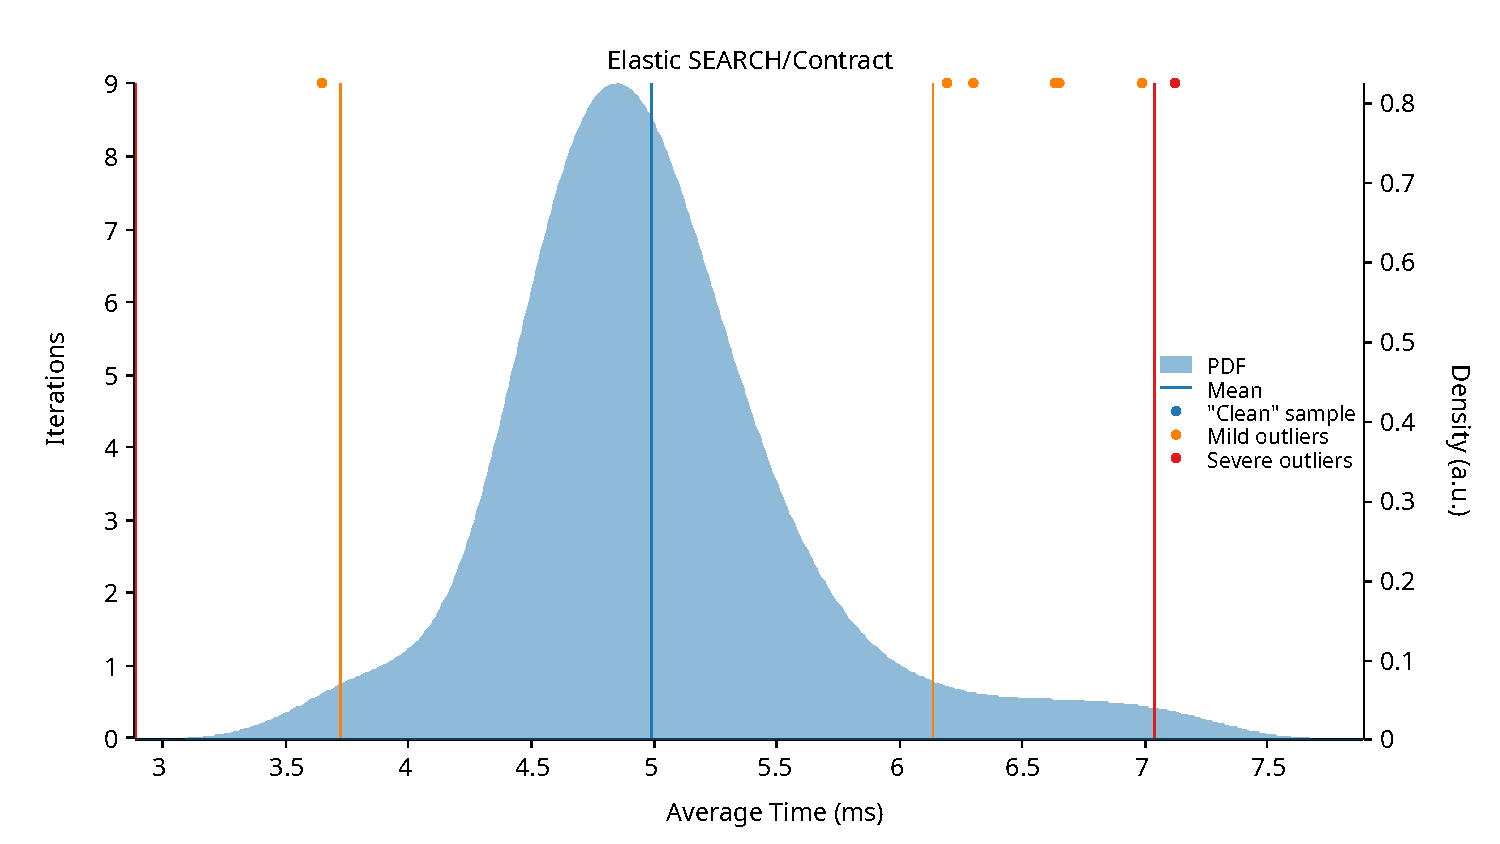
\includegraphics[width=1\linewidth]{images/benchmark/SEARCH/contract/density.pdf}
	\caption{Diagramma densità probabilistica richieste \texttt{evaluate} di tipo SEARCH}\label{densità contract search}
\end{figure}

\paragraph{Statistiche calcolate}
La Tabella \ref{benchmark search contract} riporta le statistiche derivanti dai benchmark. Si evidenzia un tempo medio di esecuzione pari a 4.9 ms e una deviazione standard pari a 600.06 µs, il che indica misurazioni molto stabili.

\begin{table}[H]
	\caption{Valutazioni statistiche SEARCH/Contract benchmark}\label{benchmark search contract}
	\centering
	\begin{tabularx} {0.9\textwidth}
		{C| c*{3}{C}} % C è un column type definito nel main
		\toprule
		\textbf{Misurazione} & \textit{Lower bound} & \textbf{Estimate}  & \textit{Upper bound} \\

		\midrule
		\textbf{Mean}        & 4.8786 ms            & \textbf{4.9931 ms} & 5.1138 ms            \\
		\textbf{Std. Dev.}   & 468.76 µs            & \textbf{600.06 µs} & 716.74 µs            \\
		\textbf{Median}      & 4.8183 ms            & \textbf{4.9212 ms} & 4.9911 ms            \\
		\textbf{\gls{MAD}}   & 312.40 µs            & \textbf{446.40 µs} & 544.85 µs            \\
		\textbf{R2}          & 0.0054919            & \textbf{0.0056929} & 0.0054707            \\

		\bottomrule
	\end{tabularx}
\end{table}

\paragraph{Diagramma Sample-Time}
La Figura \ref{iter-time contract search} illustra un diagramma che descrive il tempo impiegato da ciascun sample per completare l'esecuzione della funzione. Sono riportati 100 sample e l'altezza ne indica il tempo impiegato. Non si evidenzia nessuna dispersione significativa nelle valutazioni dei sample, sono presenti 6 outlier al di sopra del 6. Si nota come la condensazione massima di valori sia nell'intervallo temporale 4.5 e 5.5.

\begin{figure}[H]
	\centering
	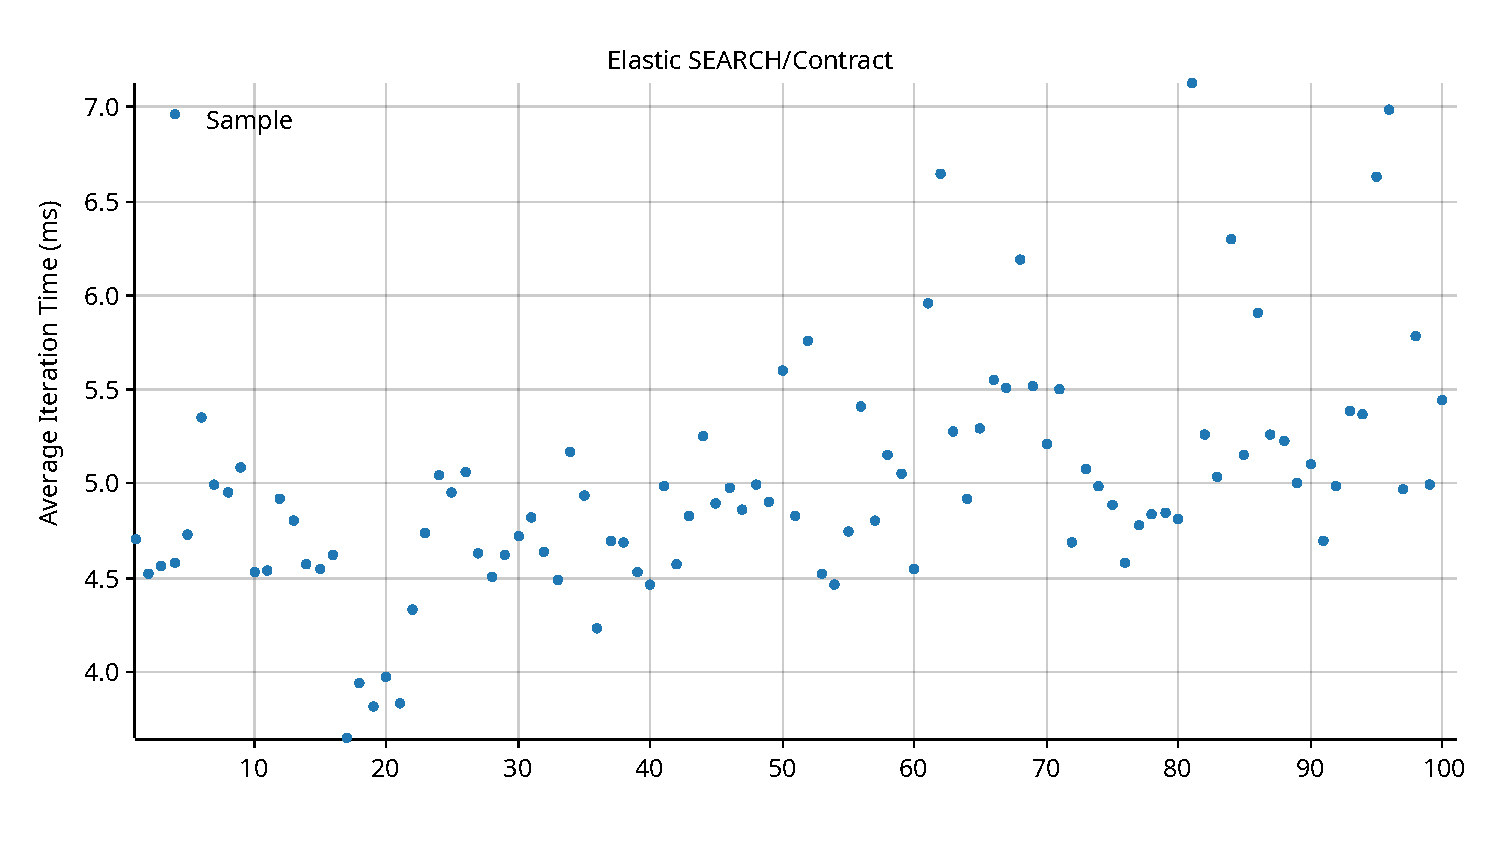
\includegraphics[width=1\linewidth]{images/benchmark/SEARCH/contract/iteration-times.pdf}
	\caption{Diagramma iteration/time richieste \texttt{evaluate} di tipo SEARCH}\label{iter-time contract search}
\end{figure}


%%%%%%%%%%%%%%%%%%%%%%%%%%%%%%%%%%%%%%%%%%%%%%%%%%%%%%%%%%%%
%%%%%%%%%%%%%%%%%%%%%%%%%%%%%%%%%%%%%%%%%%%%%%%%%%%%%%%%%%%%
\section{SQL Benchmark}
Benchmark condotto sulle funzioni \texttt{measure()} ed \texttt{evaluate()} utilizzando la Query SQL descritta nel Codice \ref{JSON query sql} che estrae due campi dall'indice filtrando sulla data.

\paragraph{Confronto funzioni benchate}
La Figura \ref{violino sql} illustra due distribuzioni di probabilità relative al tempo medio di esecuzione delle funzioni \texttt{evaluate} e \texttt{measure}.
Come nel precedente diagramma a violino, sull'asse delle ascisse è presente il tempo di esecuzione mentre su quello delle ordinate i due benchmark da confrontare.
Si può notare come le distribuzioni si concentrino introno al valore medio, 8.5 ms per le metriche e 7.6 ms per i contratti.
Si nota anche come l'ampiezza di entrambi i benchmark, ma prevalentemente di quello Metric, si discosti dal valore medio a causa di alcuni \textit{outliers} misurati, identificati ancora da una riga orizzontale che ne definisce una probabilità irrisoria.
Per concludere, l'esecuzione del benchmark sui contratti è ancora una volta stabile in quanto tutte le misurazioni hanno ottenuto valori addensati intorno ai 7.6 ms, ad eccezione di lievi outlier. 
Il benchmark sulle metriche, come osservato nei benchmark SEARCH, mostra una media leggermente più alta, intorno agli 8.5 ms, a causa di misurazioni outliers più frequenti.
\begin{figure}[H]
	\centering
	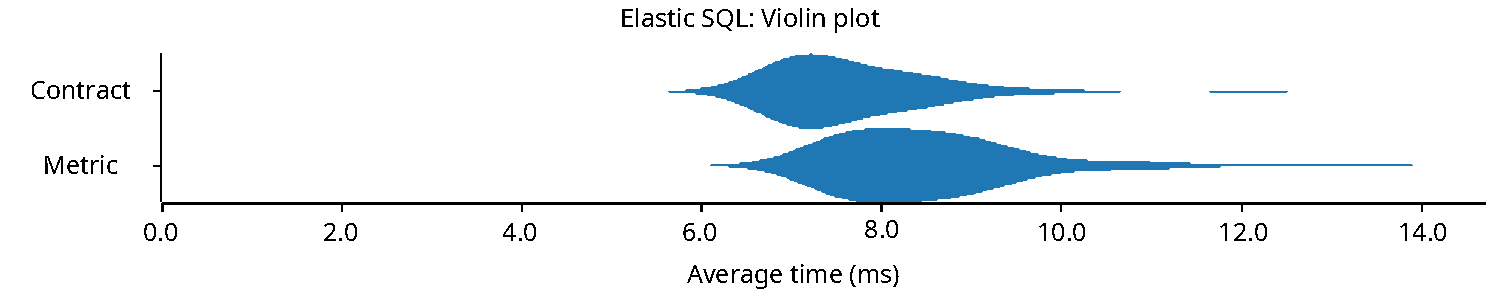
\includegraphics[width=1\linewidth]{images/benchmark/SQL/sql-violin.pdf}
	\caption{Diagramma a violino richieste di tipo SQL}\label{violino sql}
\end{figure}

%%%%%%%%%%%%%%%%%%%%%%%%%%%%%%%%%%%%%%%%%%%%%%%%%%%%%%%%%%%%
%%%%%%%%%%%%%%%%%%%%%%%%%%%%%%%%%%%%%%%%%%%%%%%%%%%%%%%%%%%%
\subsection{Metric - \texttt{measure()}}\label{section metric sql}
\paragraph{Diagramma distribuzione probabilità-tempo}
La Figura \ref{densità metric sql} mostra la distribuzione di probabilità sulle tempistiche di esecuzione del metodo \texttt{measure}.
Si evidenzia anche qui la presenza di un unico picco centrale, che si allontana leggermente dalla media di 8.5 ms a causa della presenza di lievi outliers, al di sopra dei 10.8 ms, che influiscono lievemente sulla valutazione complessiva.
La maggior parte dei dati è concentrata tra 7 e 10 ms.

\begin{figure}[H]
	\centering
	
\includegraphics[width=1\linewidth]{images/benchmark/SQL/metric/density.pdf}
	\caption{Diagramma densità probabilistica richieste \texttt{measure} di tipo SQL}\label{densità metric sql}
\end{figure}

\paragraph{Statistiche calcolate}
Nella Tabella \ref{benchmark sql metric} sono elencate le statistiche ottenute tramite i benchmark, con una media del tempo di esecuzione pari a 8.5 ms e una deviazione standard rispetto tale valore pari a 1.07 ms.
\begin{table}[ht!]
	\caption{Valutazioni statistiche SQL/Metric benchmark}\label{benchmark sql metric}
	\centering
	\begin{tabularx} {0.9\textwidth}
		{C| c*{3}{C}} % C è un column type definito nel main
		\toprule
		\textbf{Misurazione} & \textit{Lower bound} & \textbf{Estimate}  & \textit{Upper bound} \\

		\midrule
		\textbf{Mean}        & 8.3206 ms            & \textbf{8.5206 ms} & 8.7393 ms            \\
		\textbf{Std. Dev.}   & 812.45 µs            & \textbf{1.0723 ms} & 1.3265 ms            \\
		\textbf{Median}      & 8.0902 ms            & \textbf{8.3803 ms} & 8.6017 ms            \\
		\textbf{\gls{MAD}}   & 737.19 µs            & \textbf{895.16 µs} & 1.1394 ms            \\
		\textbf{R2}          & 0.0040924            & \textbf{0.0042356} & 0.0040656            \\

		\bottomrule
	\end{tabularx}
\end{table}

\paragraph{Diagramma Sample-Time}
La Figura \ref{iter-time metric sql} presenta un diagramma che raffigura i tempi di esecuzione della funzione per ciascun sample. Tra i 100 sample presenti non emerge nessuna dispersione significativa nelle valutazioni; sono presenti 5 outlier al di sopra del 10.8. Si evidenzia come la maggior parte dei valori è concentrata nell'intervallo temporale 7 e 10.
\begin{figure}[H]
	\centering
	
\includegraphics[width=1\linewidth]{images/benchmark/SQL/metric/iteration-times.pdf}
	\caption{Diagramma iteration/time richieste \texttt{measure} di tipo SQL}\label{iter-time metric sql}
\end{figure}

%%%%%%%%%%%%%%%%%%%%%%%%%%%%%%%%%%%%%%%%%%%%%%%%%%%%%%%%%%%%
%%%%%%%%%%%%%%%%%%%%%%%%%%%%%%%%%%%%%%%%%%%%%%%%%%%%%%%%%%%%
\subsection{Contract - \texttt{evaluate()}}\label{section contract sql}
\paragraph{Diagramma distribuzione probabilità-tempo}
La Figura \ref{densità contract sql} rappresenta la distribuzione di probabilità del tempo richiesto per l'esecuzione del metodo \texttt{evaluate}.
Si osserva un unico picco centrale che si discosta leggermente dalla media, il cui valore è 7.6 ms. 
Questa variazione è ancora una volta influenzata dalla presenza di outliers sopra i 9.8 ms, che seppur presenti in minima frequenza hanno un impatto sulla valutazione finale.
La concentrazione principale dei valori si colloca tra 6.5 e 9 ms; si notano anche i due valori outlier al di sopra dei 10 ms.
\begin{figure}[H]
	\centering
	
\includegraphics[width=1\linewidth]{images/benchmark/SQL/contract/density.pdf}
	\caption{Diagramma densità probabilistica richieste \texttt{evaluate} di tipo SQL}\label{densità contract sql}
\end{figure}

\paragraph{Statistiche calcolate}
La Tabella \ref{benchmark sql contract} mostra i risultati statistici dei benchmark effettuati, i quali mostrano una media del tempo di esecuzione pari a 7.6 ms e una deviazione standard rispetto tale valore pari a 882.01 µs.
\begin{table}[ht!]
	\caption{Valutazioni statistiche SQL/Contract benchmark}\label{benchmark sql contract}
	\centering
	\begin{tabularx} {0.9\textwidth}
		{C| c*{3}{C}} % C è un column type definito nel main
		\toprule
		\textbf{Misurazione} & \textit{Lower bound} & \textbf{Estimate}  & \textit{Upper bound} \\

		\midrule
		\textbf{Mean}        & 7.4923 ms            & \textbf{7.6578 ms} & 7.8354 ms            \\
		\textbf{Std. Dev.}   & 666.71 µs            & \textbf{882.01 µs} & 1.1105 ms            \\
		\textbf{Median}      & 7.3017 ms            & \textbf{7.4661 ms} & 7.6194 ms            \\
		\textbf{\gls{MAD}}   & 505.58 µs            & \textbf{729.81 µs} & 898.74 µs            \\
		\textbf{R2}          & 0.0102391            & \textbf{0.0105995} & 0.0101868            \\

		\bottomrule
	\end{tabularx}
\end{table}

\paragraph{Diagramma Sample-Time}
Nella Figura \ref{iter-time contract sql} viene raffigurato un diagramma che rappresenta il tempo di esecuzione di ciascun sample per terminare la funzione. 
Su 100 sample presenti, di cui l'altezza ne indica il tempo impiegato, non si nota nessuna dispersione significativa nelle valutazioni.
\'E il benchmark con il minor numero di outlier, solo 2 sono presenti sopra al valore 9.8. I valori si condensano tutti nell'intervallo temporale 6.5 e 9.

\begin{figure}[H]
	\centering
	
\includegraphics[width=1\linewidth]{images/benchmark/SQL/contract/iteration-times.pdf}
	\caption{Diagramma iteration/time richieste \texttt{evaluate} di tipo SQL}\label{iter-time contract sql}
\end{figure}
%%%%%%%%%%%%%%%%%%%%%%%%%%%%%%%%%%%%%%%%%%%%%%%%%%%%%%%%%%%%
%%%%%%%%%%%%%%%%%%%%%%%%%%%%%%%%%%%%%%%%%%%%%%%%%%%%%%%%%%%%







\chapter{Discussione}\label{discussione}
In questa sezione verranno analizzati i risultati ottenuti dai test sulle performance del sistema illustrati nel capitolo precedente. L'obbiettivo è quello di fornire un commento sui risultati ottenuti e sulle motivazioni di situazioni anomale.

\section{SEARCH Benchmark}
Verrà effettuato un breve commento sui risultati e sui diagrammi ottenuti dai benchmark di SEARCH.

\paragraph{Metric - \texttt{measure()}}
Il benchmark visto nella Sezione \ref{section metric search} con la relativa Figura \ref{densità metric search} è quello con il maggior numero di outlier, 14/100, tutti di tipo ``severe outlier''.
\'E interessante notare dalla Figura \ref{iter-time metric search} come siano stati tutti i primi sample eseguiti a produrre questi valori particolarmente alti in un istanza di tempo circoscritta e consecutiva.
La motivazione più plausibile di questa situazione è dovuta ad un picco iniziale nella latenza di rete in quanto successivamente si trovano valori accettabili ed in linea con i restanti benchmark.

\paragraph{Contract - \texttt{evaluate()}}
Il benchmark visto nella Sezione \ref{section contract search} con la relativa Figura \ref{densità contract search}, a differenza del primo, presenta una distribuzione molto più uniforme e compatta, con tendenza ad una Normale o Gaussiana, in quanto tutti i valori tendono a concentrarsi attorno ad un singolo valore medio. \'E una distribuzione ottenibile dalla media, che ne definisce il picco centrale, e dalla deviazione standard che ne definisce la dispersione attorno ad essa.
La Figura \ref{iter-time contract search} presenta una situazione molto simile a quella del diagramma del precedente benchmark. Sono presenti outliers, più lievi dei precedenti, che però non si trovano all'inizio dell'esecuzione ma oltre il 50esimo sample.

Questa situazione avvalora maggiormente la nostra ipotesi che la fluttuazione dei risultati dei benchmark e questi outliers dipendano dalle condizioni della rete.
Se in tutti i benchmark avessimo trovato un ritardo iniziale allora la causa sarebbe stata molto probabilmente il mancato riscaldamento o la perdita dei valori in cache.


\section{SQL Benchmark}
Verrà effettuato un breve commento sui risultati e sui diagrammi ottenuti dai benchmark di SQL.

\paragraph{Metric - \texttt{measure()}}
Il benchmark visto nella Sezione \ref{section metric sql} con la relativa Figura \ref{densità metric sql} presenta anch'esso una distribuzione abbastanza compatta e simile a una Normale o Gaussiana in quanto tutti i valori tendono a concentrarsi attorno ad un singolo valore medio.
La Figura \ref{iter-time metric sql} rispetto alle due precedenti non presenta evidenza particolari di latenza tranne alcuni outliers distribuiti.


\paragraph{Contract - \texttt{evaluate()}}
Nel benchmark visto nella Sezione \ref{section contract sql} con la relativa Figura \ref{densità contract sql}, come nel caso precedente, i valori tendono a concentrarsi attorno ad un singolo valore medio
presentando una distribuzione Gaussiana.
Si può notare come la densità nella zona di outliers sia la minore rispetto a tutti i benchmark precedenti.
La Figura \ref{iter-time contract sql} presenta un'esecuzione pressoché ottima in quanto sono presenti solo due outliers e gli altri valori si condensano all'interno di un range ristretto.
\'E il benchmark avvenuto con la condizione di rete ideale.


\section{Valori anomali}\label{valori anomali}
Un'aspetto abbastanza particolare notato in entrambi i benchmark, come si può vedere nelle Tabelle \ref{benchmark search metric}, \ref{benchmark search contract} per la SEARCH e nelle Tabelle \ref{benchmark sql metric} e \ref{benchmark sql contract} per SQL, è il fatto che l'esecuzione dei metodi \texttt{evaluate()} è mediamente 1 ms più breve dell'esecuzione del metodo \texttt{measure()}.
Nei benchmark di SEARCH \textit{metric} si hanno come valori medi 6.2~ms mentre in quelli \textit{contract} si hanno 4.9 ms.
Nei benchmark di SQL \textit{metric} si hanno come valori medi 8.5 ms mentre in quelli di \textit{contract} si hanno 7.6 ms. \\
Questo risulta essere abbastanza controintuitivo e contro le nostre aspettative in quanto il metodo \texttt{evaluate()} contiene al suo intero un'invocazione al metodo \texttt{measure()} e dei controlli effettuati sui risultati; logicamente dovrebbe impiegare un tempo maggiore.

Per indagare su questi risultati sono state eseguite altre serie di benchmark. Si è notato come i valori medi di esecuzioni oscillino parecchio tra un test e l'altro riscontrando miglioramenti o regressioni fino al 50\% del valore.
Le oscillazioni si suppone ancora una volta siano dovute alla latenza introdotta dalla comunicazione di rete in quanto non si presentano in modo prevedibile nei sample.
In tutti i test successivi non si è riscontrato nulla di anomalo in merito ai tempi di esecuzione, alle statistiche e ai grafici. Si sottolinea sempre il tempo minore impiegato dalle funzioni \texttt{evaluate()}.

L'ultima prova effettuata per dare una spiegazione ai risultati è quella che ci ha fornito maggiori punti su cui riflettere.
Abbiamo provato a effettuare i benchmark con l'ordine invertito rispetto alle fasi discusse nel capitolo precedente, sono state benchate prima le funzioni \texttt{evaluate()} e poi le \texttt{measure()}. \'E stata provata questa modalità per andare a scartare l'ipotesi che dipendesse dalla cache di Elasticsearch.
Si è visto invece, al contrario di come ci si aspettava, che l'ordine con cui vengono effettuati i benchmark va ad influire sulle prestazioni medie finali, ciò è dovuto probabilmente ad un salvataggio dei valori in cache. Elasticsearch utilizza un doppio sistema di caching: da un lato si appoggia sul caching delle pagine del file-system e dall'altro sfrutta un proprio sistema di caching interno contenente i risultati delle query; il secondo benchmark dunque è lievemente favorito rispetto al primo.
Si nota come il primo metodo eseguito presenta sempre un rallentamento di qualche decimo di millisecondo.

\begin{figure}[htb]
	\centering
	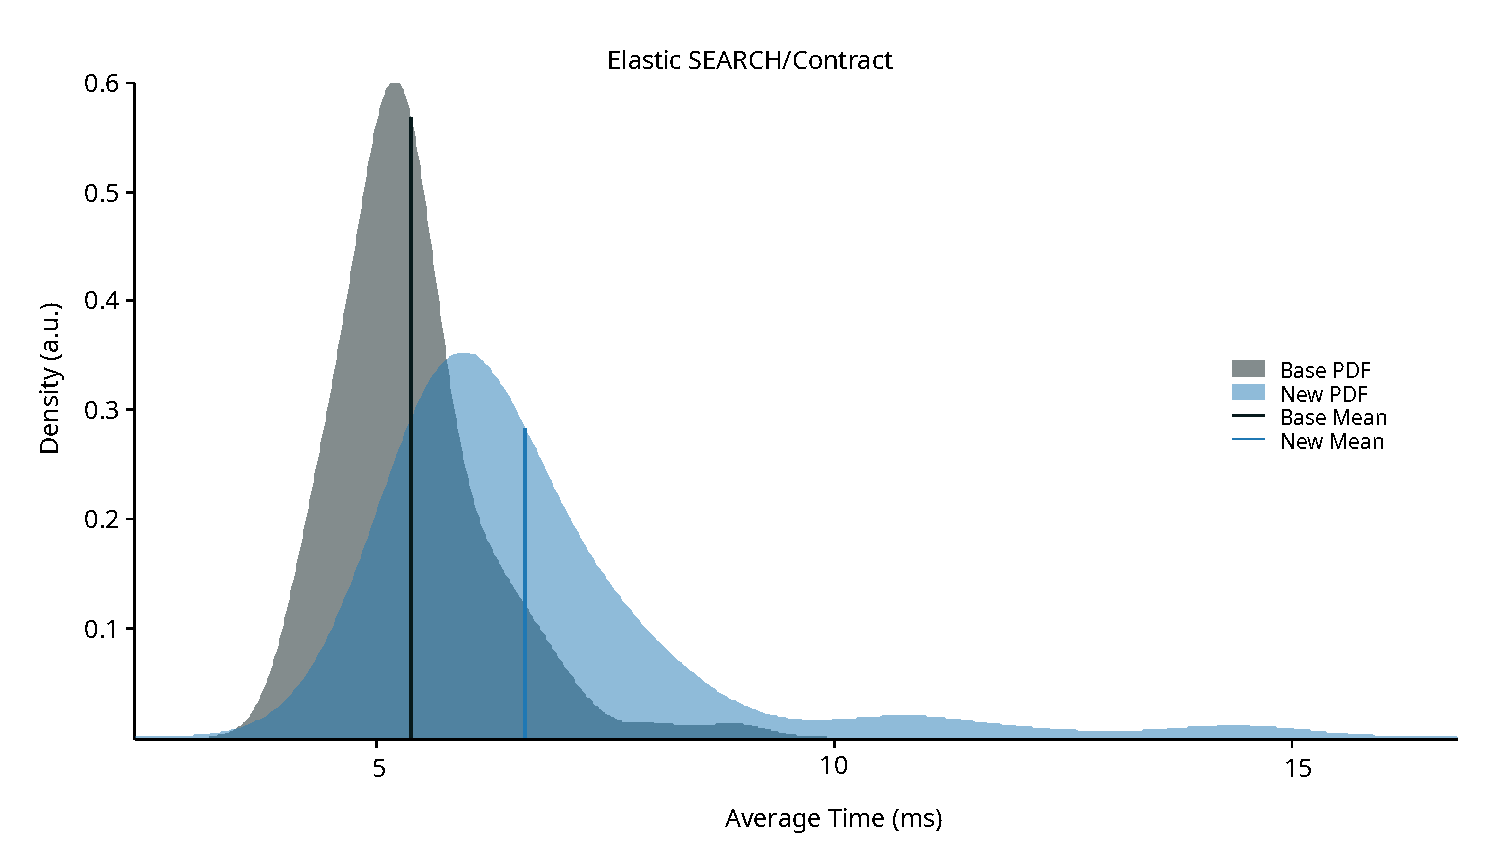
\includegraphics[width=1\linewidth]{images/benchmark/discussion/density-change.pdf}
	\caption[Diagramma confronto densità probabilistica]{Diagramma confronto densità probabilistica richieste \texttt{evaluate} di tipo SEARCH}\label{densità test}
\end{figure}

Nella Figura \ref{densità test} viene colorato di grigio la densità del metodo \texttt{evaluate()} eseguito dopo il metodo \texttt{measure()} mentre in azzurro la densità quando viene eseguito prima. Si nota come l'area azzurra è più spostata verso destra, risultando in un tempo medio lievemente maggiore.

\begin{figure}[htb]
	\centering
	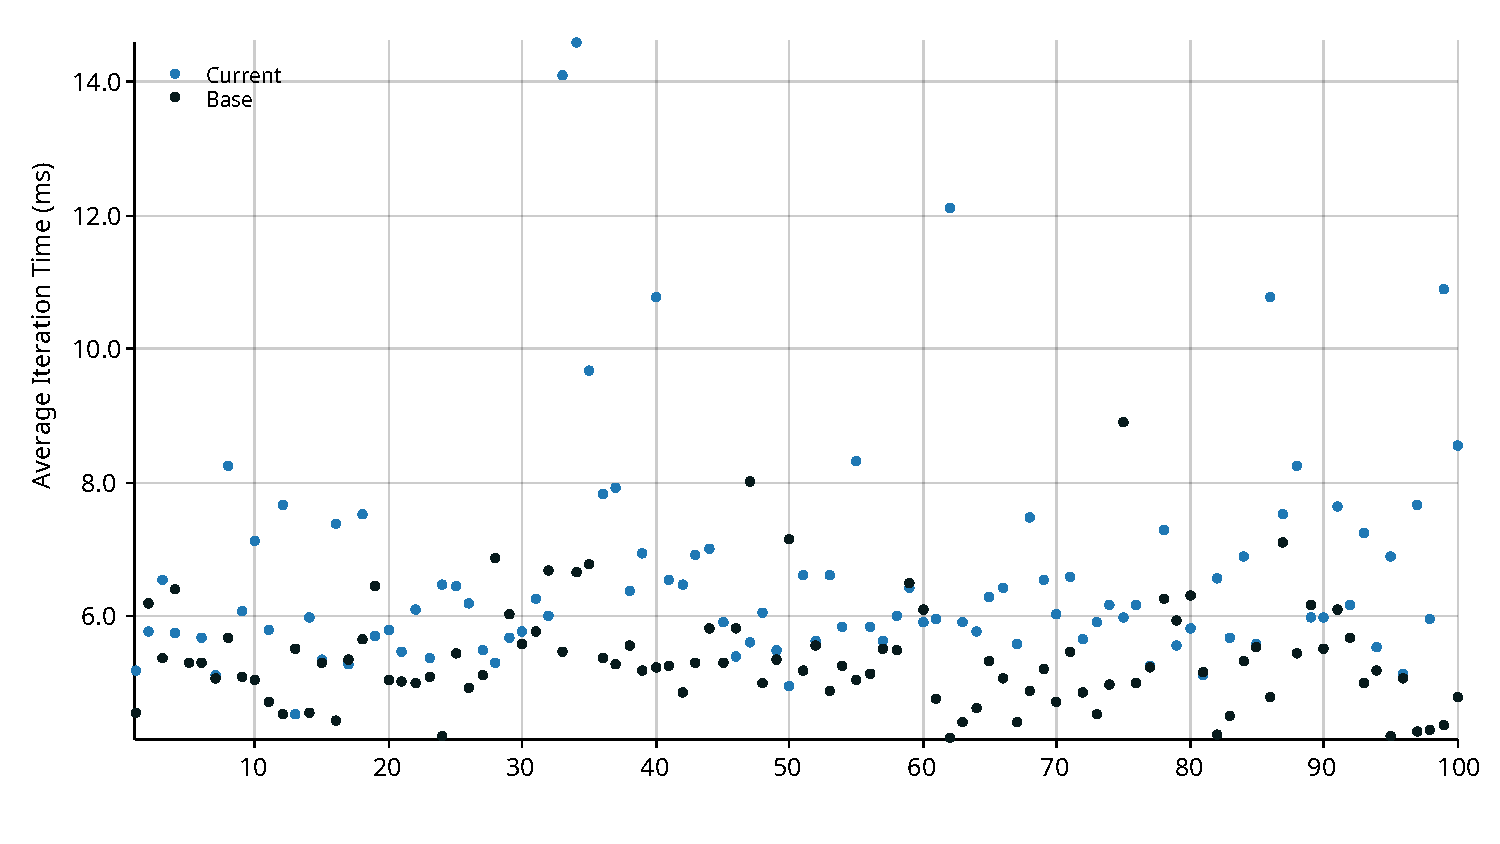
\includegraphics[width=1\linewidth]{images/benchmark/discussion/iteration-times-change.pdf}
	\caption[Diagramma confronto iteration/time]{Diagramma confronto iteration/time richieste \texttt{evaluate} di tipo SEARCH}\label{iteration-time test}
\end{figure}

La Figura \ref{iteration-time test} evidenzia lo stesso concetto mostrando però singolarmente i sample a confronto. I test in cui \texttt{contract()} viene eseguito dopo \texttt{measure()} sono rappresentati da pallini blu scuro mentre quelli eseguiti invertiti sono rappresentati da pallini azzurri. Si nota anche qua come generalmente i pallini azzurri stiano al di sopra di quelli blu.


%intendo l'overhead della cache di elastic
In conclusione, si può affermare che l'overhead introdotto dal mancato hit nella cache di Elasticsearch è talmente piccolo che risulta essere trascurabile ai fini della valutazione delle performance, mentre il fattore che causa maggiore oscillazione si dimostra quindi essere la rete e la latenza di trasmissione.
Si dimostra anche l'efficienza del sistema, sebbene effettui controlli molto semplici, e si può affermare che l'overhead introdotto dalla computazione risulta essere irrilevante rispetto a quello introdotto dalla rete.



\chapter{Conclusioni}\label{conclusione}
%%%%CONTENUTI%%%%
% thesis
% methodology
% experiments e results
% future work

%\section{Obbiettivo - Domanda - TODO}
%Nelle conclusioni vanno ripresi domanda/problema e gaps + obiettivi in modo puntuale; Non ci devono essere ri-definizioni 
%nelle conclusioni si dice questi gap li ho coperti più o meno, questi obbiettivi li ho raggiunti più o meno

Questa tesi si occupa di soddisfare alcune delle esigenze e limitazioni, introdotte dalla decentralizzazione e dalla conseguente adozione di architetture distribuite basate su microservizi, legate al monitoring.

L'Obiettivo \nameref{o1: estensione ae} di questa tesi, che va a risolvere il primo Gap \nameref{g1: generalizzabilità}, è l'estensione di un sistema generico e altamente scalabile, capace di raccogliere dati da diverse fonti e di effettuare valutazioni basate su contratti predefiniti.
Viene quindi integrato il sistema presente con Elasticsearch, uno strumento di monitoring, rendendo possibile l'esecuzione di metriche per ottenere \textit{measurements} dal servizio di backend e la valutazione di contratti basati sulle \textit{evidence} ottenute.

Il secondo Obbiettivo \nameref{o2: contratti}, che va a risolvere i successivi due Gaps \nameref{g2: performance e PNF} e \nameref{g3: contratti avanzati}, riguarda l'implementazione di contratti specifici e più strutturati che definiscono le modalità per verificare \gls{PNF} sulla base delle \textit{evidence} ottenute.
Oltre agli aspetti prestazionali del sistema è possibile la valutazione di proprietà specifiche sui dati ottenuti grazie a delle regole \textit{taylor-made} sviluppate nei contratti, ottenendo così un sistema di \textit{Assurance} più flessibile e completo.

L'ultimo Obbiettivo \nameref{o3: valutazione sperimentale} infine viene soddisfatto implementando benchmark che ne valutano l'efficienza complessiva.

\section{Metodologia e Funzionamento}
La \emph{metodologia di Assurance} adottata, illustrata nel Capitolo \ref{assurance methodology}, si basa sulla definizione di due componenti base dell'intera infrastruttura, le \emph{metriche} e i \emph{contratti}, per la verifica di \gls{PNF}, ovvero vincoli al modo in cui il sistema implementa e fornisce le sue funzionalità.
I dati vengono raccolti dagli endpoint del sistema target attraverso l'esecuzione di Metriche focalizzate sulla misurazione di un comportamento specifico. 
Una volta raccolte le \textit{evidence} o prove, i Contratti ne specificano come deve avvenire la valutazione.

Il \emph{processo di Assurance} utilizzato, illustrato nel Capitolo \ref{assurance process}, si suddivide in 4 fasi eseguite ciclicamente.
\textit{Evaluation mapping}, identificazione delle metriche e dei contratti necessari per verificare le proprietà desiderate. \textit{Measurement collection}, valutazione delle metriche e salvataggio delle evidence.
\textit{Contract evaluation}, calcolo del risultato booleano dei contratti applicati alle evidence raccolte sulla base delle condizioni espresse al loro interno. \textit{Report composition}, i risultati vengono aggregati in un report machine-readable che contiene l'esito della verifica e le evidence su cui si basa. 

Il \emph{funzionamento dell'Assurance-Engine}, illustrato nel Capitolo \ref{funzionamento ae}, prevede che un utente interagisca con il metodo POST di una delle \gls{API} esposte per dare inizio all'esecuzione.
L'esecuzione rispecchia la suddivisione fatta nel processo di Assurance e ne vengono illustrati i 3 punti principali.
\textit{Measurement collection}, viene utilizzato il metodo \texttt{measure()} per ottenere prove da un target o per inviare richieste personalizzate; i dati raccolti vengono identificati come \textit{measurements} e costituiscono le \textit{evidence} necessarie per la valutazione del sistema. Si esegue infine un parsing della risposta JSON per estrarre campi e valori desiderati.
\textit{Contract evaluation}, vengono eseguiti controlli booleani, tramite il metodo \texttt{evaluate()}, confrontando le measurements ottenute con i parametri del contratto; i risultati dei vari controlli vengono infine aggregati per stabilire se la proprietà oggetto di verifica è stata soddisfatta.
\textit{Report composition}, i risultati finali vengono formalizzati in una struttura contenente le evidence, il risultato e il timestamp per poi essere inviate in formato JSON all'utente che ha avviato la richiesta.

\section{Esperimenti e risultati}
%OK-riassunto dei risultati ottenuti (quanto bene ha funzionato, ci si può rifare alla discussione)
Come mostrato nel Capitolo \ref{implementazione} e verificato nel Capitolo \ref{esperimenti} sono stati condotti 2 benchmark per valutare le performance del sistema sviluppato sull'ottenimento di metriche e sulla valutazione di contratti. Il primo benchmark esegue query nel Query \gls{DSL} di Elastic mentre il secondo le esegue in SQL.
Entrambi valutano le performance di esecuzione dei metodi \texttt{measure()} ed \texttt{evaluate()}, rispettivamente di Metriche e Contratti.
I risultati emersi hanno dimostrato una grande efficienza del sistema, eseguendo le query proposte in tempi tra i 6 e gli 8 millisecondi. \\
Data la differenza anomala di tempistiche tra i due metodi, illustrata nella Sezione \ref{valori anomali}, si è notato come Elasticsearch performi leggermente meglio quando possiede le query e i risultati in cache, con miglioramenti nell'ordine dei decimi di millisecondo, trascurabili in termini di valutazione.
Si sono notate anche oscillazioni nelle performance tra benchmark eseguiti consecutivamente con regressioni e miglioramenti fino al 50\%, rientrando però sempre in un range di efficienza accettabile. Analizzando i sample dei benchmark è stata associata alla rete la causa principale di questa latenza variabile, in quanto non si presenta in modo prevedibile tra le richieste.\\
Il sistema sviluppato permette quindi di effettuare \textit{verifiche di Assurance} tramite dati collezionati all'interno di Elasticsearch con estrema efficienza e poco overhead. Si è notato come il tempo computazionale di esecuzione dei metodi \texttt{measure()} o \texttt{evaluate()}, i quali assolvono rispettivamente al compito di ottenere prove e verificare contratti complessi per garantire \gls{PNF}, sia proporzionalmente irrisorio rispetto alla latenza introdotta dalla rete che ne definisce il tempo medio di esecuzione. Di conseguenza, si ottiene un sistema estremamente efficiente che si pone come intermediario generando un overhead trascurabile.


%%%%%%%%%%%%%%%%%%%%%%%%%
\section{Future Work}
In questa tesi sono state poste le basi per un \textit{sistema di assurance} per sistemi distribuiti scalabile e generico. Il sistema attualmente realizzato si presta come struttura di partenza per nuovi possibili sviluppi e migliorie.

\paragraph{Nuove integrazioni}
Il framework descritto, grazie alla sua struttura modulare e alla funzione di intermediario, può essere facilmente esteso per integrare nuove sorgenti di dati oltre a quelle già supportate, come Elasticsearch e Prometheus, e per eseguire specifiche \textit{probe ad-hoc}. 
Questo consente la creazione di un sistema unificato in grado di interfacciarsi con molteplici soluzioni di monitoring e storage comunemente utilizzate.
L'obiettivo finale è sviluppare una piattaforma centralizzata in grado di raccogliere e gestire dati da diverse fonti, migliorando la visibilità e il controllo su vari sistemi informativi.
La modularità è il fattore chiave di questa soluzione che ne permette una facile estensibilità e una maggiore versatilità nel rispondere a esigenze diverse.


\paragraph{Contratti e probe avanzate}
Attualmente, le \gls{API} esposte dal sistema offrono solo una gamma limitata di funzionalità.
Una direzione di sviluppo promettente è l'espansione delle \gls{API} esposte per supportare funzionalità più complesse e specifiche.
Tra questi sviluppi futuri ricade la generazione di nuovi contratti, sempre più strutturati e complessi, sui dati raccolti dalle varie sorgenti per verificare \gls{PNF}.
Allo stesso modo, si possono sviluppare probe che eseguono test più sofisticati su comportamenti dei sistemi target.
L'obbiettivo è ottenere un sistema più robusto, che permetta di effettuare una vasta gamma di controlli, sempre più fini, sulla base del target scelto per verificare proprietà specifiche.

\paragraph{Contratti su sistemi reali}
Finora, il sistema è stato testato in ambienti controllati o sperimentali, il cluster del laboratorio, dove si è comportato come previsto.
La fase successiva consiste nell'andare ad applicarlo ad un caso di studio reale, monitorando un sistema di produzione con traffico e carichi effettivi; è un passaggio cruciale per verificare come il framework gestisce situazioni reali, incluse eventuali anomalie o casi limite non riscontrati negli ambienti sperimentali.
Inoltre, ciò consentirà di eseguire un'analisi comparativa tra i benchmark prestazionali effettivi e quelli sperimentali, facilitando l'individuazione di aree di ottimizzazione e potenziali miglioramenti.

\paragraph{Scalabilità}
Il sistema è stato progettato per essere scalabile, senza necessità di amministrazione aggiuntiva o overhead.
Per verificare effettivamente quanto bene il framework possa scalare, si possono eseguire una serie di test che misurano le performance ottenute con diverse repliche deployate dell'assurance-agent.
Questo tipo di test fornirà dati concreti sulle performance di un sistema scalato su varie istanze e permetterà di verificare o meno l'assunzione teorica della facilità di scalabilità fatta nella sezione sulla replicabilità.



% \appendix
% \include{sections/appendix.tex}

\backmatter{}
%\printnoidxglossary
\printglossary[
	type=acronym,
	style=mcolindex,
	nonumberlist
]
%\addcontentsline{toc}{chapter}{Acronimi}

% BIBLIOGRAPHY
\bibliographystyle{IEEEtran}
\bibliography{biblio}

\end{document}
